%------------------------------------------
% README
%------------------------------------------
% MSc. CAVE latex template
%
% This is a modification of my thesis template, so there may be some things you want to remove.
% Each chapter is in a separate latex file. Those files are included using \input
% You can keep everything in one file by replacing the line "\input{...}" by the content of your chapter 
% Separate files are made so that you can compile chapters independently. Latex can be long to compile large documents
% if your thesis is not too long, then you should probably keep everything in one file.

% I use a lot of margin and padding. Feel free to change it in format-setup. If you have additional package, you can add them in format-setup.
% You can change practically everything in latex, just google it, there are always plenty of answers.


\newcommand{\isEmbedded}{true}


\documentclass[12pt]{report}
	
% FONT RELATED
%\usepackage{times} %Move to times font
\usepackage[labelfont=bf,textfont=it]{caption}
\usepackage[utf8]{inputenc}

% LINKS, PAGE OF CONTENT, REF AND CROSS-REF, HEADERS/FOOTERS
\usepackage[hidelinks]{hyperref}
\usepackage{fancyhdr}
\usepackage{acronym}

% FIGURES, GRAPHICS, TABLES
\usepackage{graphicx}
\usepackage{parskip}
%\usepackage{subfigure}
\usepackage{subfig}
\usepackage{wrapfig}
\usepackage{subfloat}

% COLOURS, TEXT AND FORMATTING
\usepackage{array}
\usepackage{color}
\usepackage{setspace}
\usepackage{longtable}
\usepackage{multirow}

% ADVANCED MATHS, PSEUDO-CODE
\usepackage{amsmath}
\usepackage{alltt}
\usepackage{amsfonts}

% ALGORITHMS
\usepackage{algorithm}
\usepackage{algorithmic}

% LANDSCAPE FOR CLASS DIAGRAM
\usepackage{pdflscape}

% BIBLIOGRAPHY
\usepackage[authoryear]{natbib}
\bibpunct{(}{)}{;}{a}{,}{,}

% USE IN DISSER:

\setlength\oddsidemargin{0.85cm}
\setlength\evensidemargin{0.85cm}

\setlength\textheight{21.0cm}
\setlength\textwidth{15.0cm}

% indent at each new paragrapg
\setlength\parindent{0.5cm}

\setlength\topmargin{-0.2in}
\renewcommand{\baselinestretch}{1.3}

%REPORT

%\setlength\oddsidemargin{1cm}
%\setlength\evensidemargin{0.3in}
%%\setlength\headsep{2.5in}
%
%\setlength\textheight{9.0in}
%\setlength\textwidth{5.5in}
%
%% indent at each new paragrapg
%\setlength\parindent{0.5cm}
%
%%\setlength{\parskip}{10.5ex}
%
%\setlength\topmargin{-0.2in}

%\newcommand{\HRule}{\rule{\linewidth}{0.5mm}}
\newcommand{\HRule}{\rule{\linewidth}{0.0mm}}

% Color definitions (RGB model)
\definecolor{ms-comment}{rgb}{0.1, 0.4, 0.1}
\definecolor{ms-question}{rgb}{0.4, 0.0, 0.0}
\definecolor{ms-new}{rgb}{0.2, 0.4, 0.8}



\begin{document}

% Front page

\begin{titlepage}

\begin{center}

~\\[4.0cm]
{ \huge \bfseries Crowd Simulation}\\[0.5cm]
{ \Large \bfseries based on emergent behaviours}\\[1.0cm]

{\large
\textsc{Carlos Pérez López}\\[1.5cm]


{\large August, 2013}\\[3.5cm]

%A thesis submitted in partial fulfilment of the requirements of Bournemouth University for the degree of Doctor of Philosophy
%\\[2.0cm]

\textbf{Master of Science,}\\[0.25cm]
\textbf{Computer Animation and Visual Effects}\\[1.0cm]
%\textbf{}\\[0.5cm]

\includegraphics[width=0.3\textwidth]{img/bu_logo}\\[1cm]

}

\vfill

\end{center}

\end{titlepage}

% Copyrights
\setcounter{page}{1}
\pagenumbering{roman}

% You dont need copyright declaration for your thesis
%\input{format/copyright}
%\pagebreak

% Table of contents, figures and tables.
% You NEED a table of contents
\addcontentsline{toc}{section}{Table of contents}
\tableofcontents
\pagebreak
% You can comment out list of figures and tables, it could be too much
\addcontentsline{toc}{section}{List of figures}
\listoffigures
\pagebreak
% You can comment out list of figures and tables, it could be too much
%\addcontentsline{toc}{section}{List of tables}
%\listoftables
%\pagebreak
% No need for abbreviations, but if you use any, define them first (e.g.: We use parametric surfaces such as Non-uniform rational B-spline (NURBS). NURBS are defined by...)
%
\section*{List of Acronyms}
\addcontentsline{toc}{section}{List of Acronyms}

\begin{acronym}[NURBS ]
\acro{ADF}{Adaptively sampled Distance Field}
\acro{BRep}{Boundary representation}
\acro{CAD}{Computer-Aided Design}
\acro{CSG}{Constructive Solid Geometry}
\acro{FRep}{Function representation}
\acro{MVC}{Mean Value Coordinates}
\acro{NURBS}{Non-uniform rational B-Spline}
\acro{SDF}{Signed distance field}
\acro{STTI}{Space Time Transfinite Interpolation}
\acro{TI}{Transfinite Interpolation}
\end{acronym}

\pagebreak
%\pagebreak

\graphicspath{{./img/}}

% Abstract

\ifx\isEmbedded\undefined

\documentclass[12pt]{report}
	
% FONT RELATED
%\usepackage{times} %Move to times font
\usepackage[labelfont=bf,textfont=it]{caption}
\usepackage[utf8]{inputenc}

% LINKS, PAGE OF CONTENT, REF AND CROSS-REF, HEADERS/FOOTERS
\usepackage[hidelinks]{hyperref}
\usepackage{fancyhdr}
\usepackage{acronym}

% FIGURES, GRAPHICS, TABLES
\usepackage{graphicx}
\usepackage{parskip}
%\usepackage{subfigure}
\usepackage{subfig}
\usepackage{wrapfig}
\usepackage{subfloat}

% COLOURS, TEXT AND FORMATTING
\usepackage{array}
\usepackage{color}
\usepackage{setspace}
\usepackage{longtable}
\usepackage{multirow}

% ADVANCED MATHS, PSEUDO-CODE
\usepackage{amsmath}
\usepackage{alltt}
\usepackage{amsfonts}

% ALGORITHMS
\usepackage{algorithm}
\usepackage{algorithmic}

% LANDSCAPE FOR CLASS DIAGRAM
\usepackage{pdflscape}

% BIBLIOGRAPHY
\usepackage[authoryear]{natbib}
\bibpunct{(}{)}{;}{a}{,}{,}

% USE IN DISSER:

\setlength\oddsidemargin{0.85cm}
\setlength\evensidemargin{0.85cm}

\setlength\textheight{21.0cm}
\setlength\textwidth{15.0cm}

% indent at each new paragrapg
\setlength\parindent{0.5cm}

\setlength\topmargin{-0.2in}
\renewcommand{\baselinestretch}{1.3}

%REPORT

%\setlength\oddsidemargin{1cm}
%\setlength\evensidemargin{0.3in}
%%\setlength\headsep{2.5in}
%
%\setlength\textheight{9.0in}
%\setlength\textwidth{5.5in}
%
%% indent at each new paragrapg
%\setlength\parindent{0.5cm}
%
%%\setlength{\parskip}{10.5ex}
%
%\setlength\topmargin{-0.2in}

%\newcommand{\HRule}{\rule{\linewidth}{0.5mm}}
\newcommand{\HRule}{\rule{\linewidth}{0.0mm}}

% Color definitions (RGB model)
\definecolor{ms-comment}{rgb}{0.1, 0.4, 0.1}
\definecolor{ms-question}{rgb}{0.4, 0.0, 0.0}
\definecolor{ms-new}{rgb}{0.2, 0.4, 0.8}


\begin{document}
%\maketitle
\fi

% The begin{abstract} seems to bug the page counter
\section*{Abstract}
\addcontentsline{toc}{section}{Abstract}
\label{sec:abstract}
%\begin{abstract}

{
The use of crowds in films and games requires time and money, either hiring extra cast or animating 3D characters by keyframing. This thesis presents an approach to simulate crowds employing an agent-based model. Although many researches have been done in this field, the method proposed here has significant differences which enhance flexibility and scalability and achieve realistic results. The simulation is entirely driven by the individual script-based behaviours. In this way, the group behaviour of the crowd will emerge from the individuals; from how they interact with each other and with the environment. Hence, very complex simulations can arise from simple behaviours.
}

%\end{abstract}


\ifx\isEmbedded\undefined
% References
\addcontentsline{toc}{chapter}{References}
\bibliographystyle{ref/harvard}
\bibliography{ref/master}
\pagebreak
\end{document}
\fi
\pagebreak
% Acknoedledgements
\section*{Acknowledgements}
\addcontentsline{toc}{section}{Acknowledgements}

To my parents, who paid the bills.

\pagebreak

% Declaration -> Dont include it, unless you have something important to put in there. 
%\input{format/declaration}

\setcounter{page}{1}
\pagenumbering{arabic}
% Chapters

\ifx\isEmbedded\undefined

\documentclass[12pt]{report}
	
% FONT RELATED
%\usepackage{times} %Move to times font
\usepackage[labelfont=bf,textfont=it]{caption}
\usepackage[utf8]{inputenc}

% LINKS, PAGE OF CONTENT, REF AND CROSS-REF, HEADERS/FOOTERS
\usepackage[hidelinks]{hyperref}
\usepackage{fancyhdr}
\usepackage{acronym}

% FIGURES, GRAPHICS, TABLES
\usepackage{graphicx}
\usepackage{parskip}
%\usepackage{subfigure}
\usepackage{subfig}
\usepackage{wrapfig}
\usepackage{subfloat}

% COLOURS, TEXT AND FORMATTING
\usepackage{array}
\usepackage{color}
\usepackage{setspace}
\usepackage{longtable}
\usepackage{multirow}

% ADVANCED MATHS, PSEUDO-CODE
\usepackage{amsmath}
\usepackage{alltt}
\usepackage{amsfonts}

% ALGORITHMS
\usepackage{algorithm}
\usepackage{algorithmic}

% LANDSCAPE FOR CLASS DIAGRAM
\usepackage{pdflscape}

% BIBLIOGRAPHY
\usepackage[authoryear]{natbib}
\bibpunct{(}{)}{;}{a}{,}{,}

% USE IN DISSER:

\setlength\oddsidemargin{0.85cm}
\setlength\evensidemargin{0.85cm}

\setlength\textheight{21.0cm}
\setlength\textwidth{15.0cm}

% indent at each new paragrapg
\setlength\parindent{0.5cm}

\setlength\topmargin{-0.2in}
\renewcommand{\baselinestretch}{1.3}

%REPORT

%\setlength\oddsidemargin{1cm}
%\setlength\evensidemargin{0.3in}
%%\setlength\headsep{2.5in}
%
%\setlength\textheight{9.0in}
%\setlength\textwidth{5.5in}
%
%% indent at each new paragrapg
%\setlength\parindent{0.5cm}
%
%%\setlength{\parskip}{10.5ex}
%
%\setlength\topmargin{-0.2in}

%\newcommand{\HRule}{\rule{\linewidth}{0.5mm}}
\newcommand{\HRule}{\rule{\linewidth}{0.0mm}}

% Color definitions (RGB model)
\definecolor{ms-comment}{rgb}{0.1, 0.4, 0.1}
\definecolor{ms-question}{rgb}{0.4, 0.0, 0.0}
\definecolor{ms-new}{rgb}{0.2, 0.4, 0.8}


\graphicspath{{../img/}}
\begin{document}
%\maketitle
\fi

\chapter{Introduction}
\label{chap:intro}

Currently, the presence of crowds in visual pieces, let they be films or video games, has acquired a lot of relevance. Scenes with a crowded train station, big streets full of pedestrians, tons of animals in a flock, troops of robots, hordes of zombies or armies of warriors can be found very often in modern films and games.

In the past, not many films could afford this kind of resources in their scenes, since the only way of having more characters was actually including more characters in the cast. The use of extras highly increases the cost of a production, besides the requirement of a strict coordination and proper training in some situations. One of the reasons of the boom of big masses in films was the arrival of new technologies in computer graphics and artificial intelligence. Alongside with this, the generation and simulation of virtual crowds became a reality, saving money and time and making the use of crowds affordable to big and small studios.

Other of the reasons of the popularity of big groups of individuals featured in films is the strength they give to a shot. It is not only a matter of fact that crowds are visually stunning and their magnificence captures the attention of the audience, but also they are powerful tools to tell and enrich a story. At this point of time, it could be hard, if not impossible, to imagine the saga of the Lord of the Rings without those epic battles of tens of thousands of warriors, or imagine the breathtaking apocalyptic scenes without those milliards of zombies wandering around.

Closely tied to the idea of crowd simulation, the concept of behaviour appears. This is what gives life to the crowd and makes the spectator perceive the group nature of it. An army of brave warriors in a battlefield will find enemies and will show aggressive movements; on the other hand, on a ballroom gentlemen and ladies will dance graciously.

\begin{figure}[!h]
  \centering
  \begin{tabular}{c c}
  	\subfloat[Crowd in a train station]{\label{fig:f1}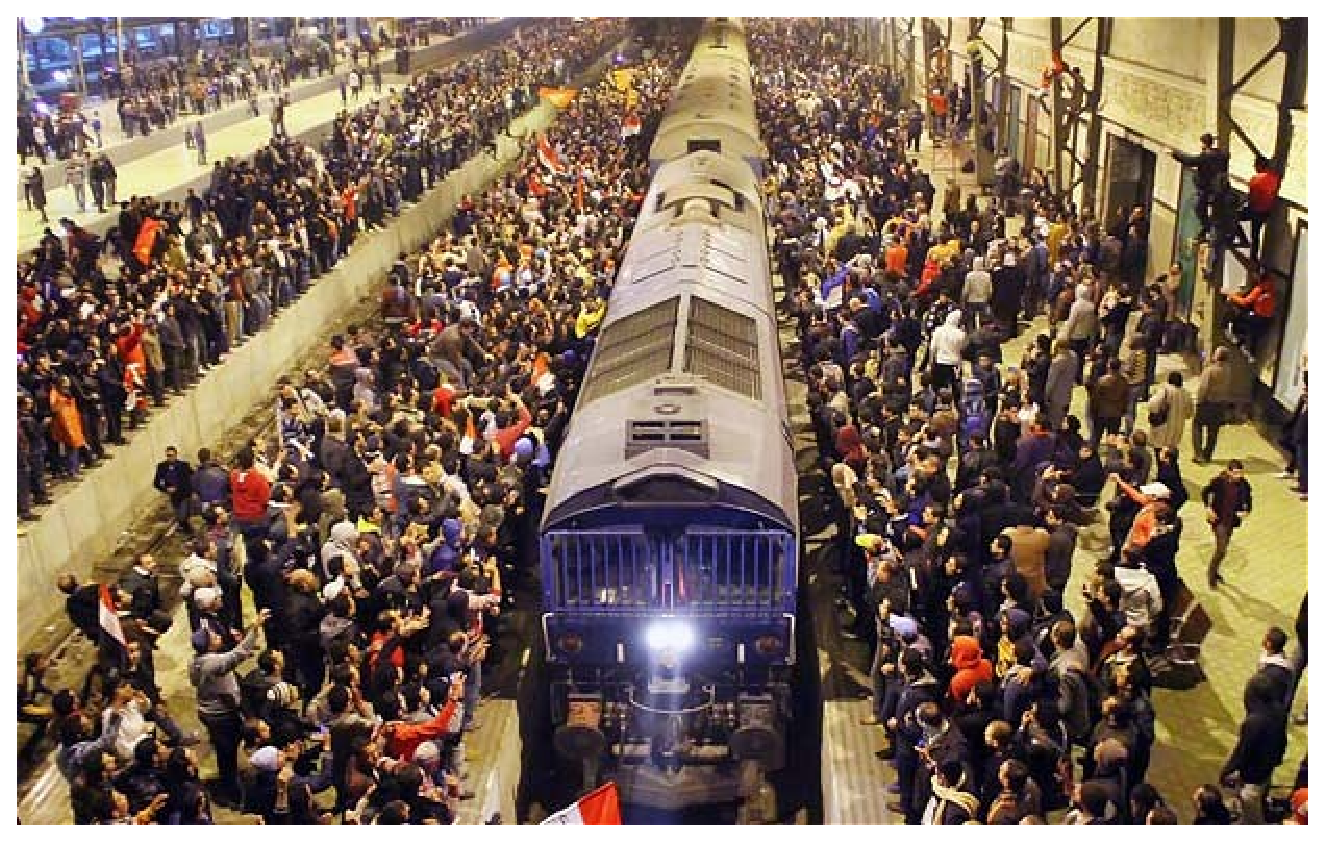
\includegraphics[scale=0.25]{crowd_train.eps}} &
 	\subfloat[Troops of droids (Star Wars)]{\label{fig:f2}\includegraphics[scale=0.18]{droids.eps}} \\
  	\subfloat[Horde of zombies (World War Z)]{\includegraphics[scale=0.1]{zombies.eps}} & 
  	\subfloat[A Battlefield (Lord of the Rings))]{
\includegraphics[scale=1.5]{battlefield.eps}} \\
  	\subfloat[A Ballroom]{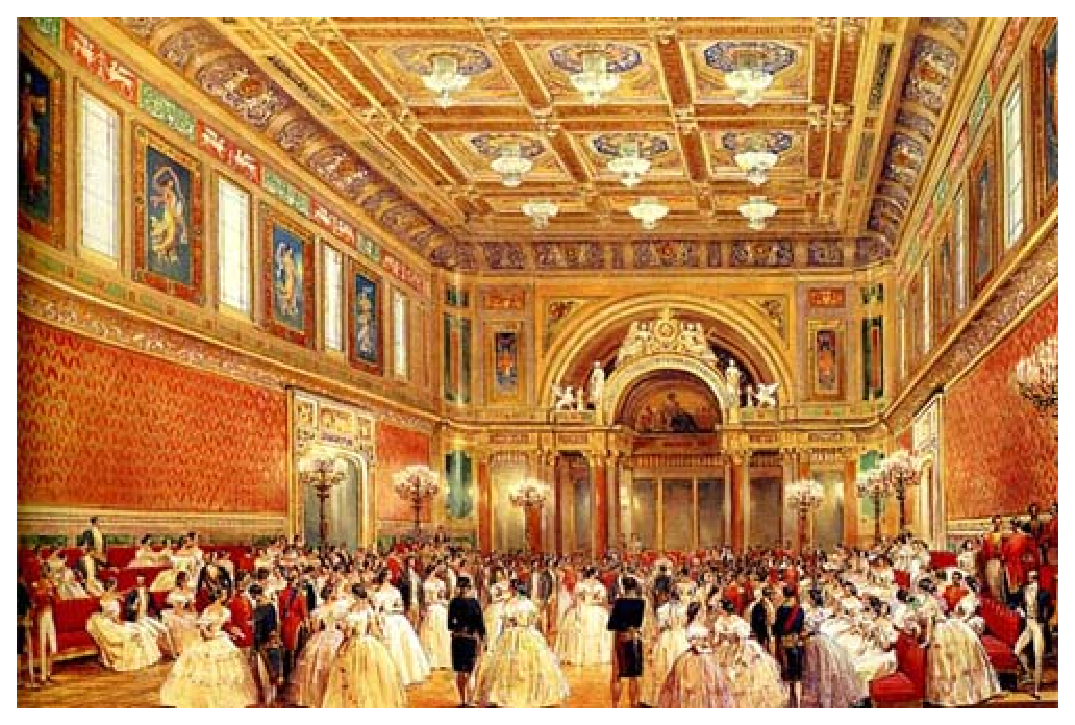
\includegraphics[scale=0.3]{ballroom.eps}} & 
  	\subfloat[One vs Many (Matrix)]{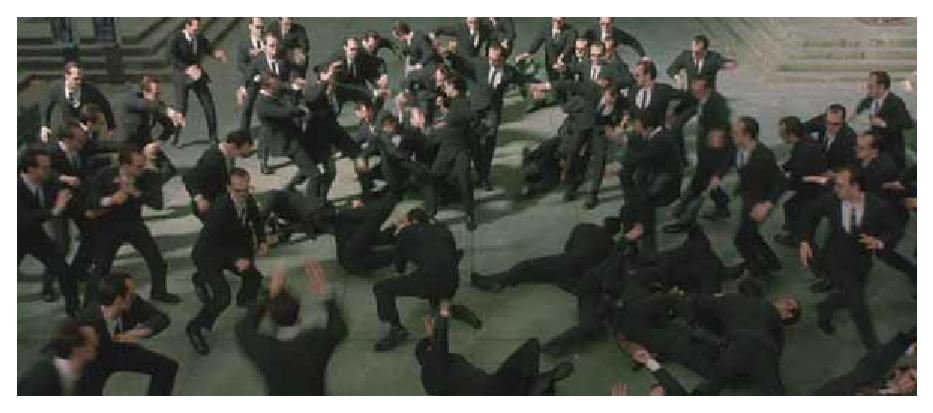
\includegraphics[scale=0.55]{matrix.eps}} \\
 \end{tabular}
  \caption{Crowd scenes}
  \label{fig:crowds}
\end{figure}

The aim of this project is to propose an approach which gives the flexibility to simulate any sort of crowd needed for a scene. Taking base on how the real world works, this method is based on the principle that the group behaviour is determined by the specific behaviours of every individual. And here is where one of the main ideas for this project appears: Emergent Behaviour.

Leonard Kleinrock, professor of computer science in UCLA, states that emergent behaviour is unanticipated behaviour shown by a system \citep{kleinrock}. Once a system is designed and defined by certain rules or mathematical equations, it may configure itself in a way that could not be anticipated. The interaction of a large number of simple individual things is very hard to predict; the complexity does not reside in the individuals, but on the way they are interconnected and they interact to each other. Professor Kleinrock proposes this example: ``we might know how a bunch of children behave when they are alone, but once you put them together in a group, you will observe behaviours that will surprise you''.

Subsequently, how a real crowd behaves is something hard to predict, and how realistic it is depends directly on how realistic each individual is.

This thesis is structured as follows:

\begin{itemize}

\item {{\bf Chapter 2: Related Work.} It explains the previous approaches in this field, the similarities and differences to the proposed method, as well as the advantages and drawbacks they present.}

\item {{\bf Chapter 3: Technical Background.} Physical concepts, flocking algorithms and the force-based virtual world model; and state machines and how they can be used to model behaviours.}

\item {{\bf Chapter 4: Agent Based Model.} This is where the current method starts to be explained into details, using a bottom-up approach. This chapter presents how agents are modeled, the parts which form them and their properties, as well as how they communicate to each other.}

\item{{\bf Chapter 5: Crowd Engine.} Here the core of the approach is introduced. It is explained how to handle the agents efficiently, how the virtual world is designed employing a physically-based approach, and how messages and collisions are faced.}

\item {{\bf Chapter 6: Applications and results.} A pipeline where this methodology might fit in a real production situation is presented. Some results of different tests will be shown in this chapter; a set of individual behaviours will be presented and the emergent behaviour observed will be explained and discussed.}

\item{{\bf Chapter 7: Application design and implementation.} The design and implementation for the application based on this approach are exposed.}

\item {{\bf Chapter 8: Conclusion.} A final concluding chapter will summarize the whole approach, mentioning the main advantages and drawbacks, as well as presenting potential lines for future work.}

\end{itemize}

\ifx\isEmbedded\undefined
% References
\addcontentsline{toc}{chapter}{References}
\bibliographystyle{../ref/harvard}
\bibliography{../ref/master}
\pagebreak
\end{document}
\fi


\ifx\isEmbedded\undefined

\documentclass[12pt]{report}
	
% FONT RELATED
%\usepackage{times} %Move to times font
\usepackage[labelfont=bf,textfont=it]{caption}
\usepackage[utf8]{inputenc}

% LINKS, PAGE OF CONTENT, REF AND CROSS-REF, HEADERS/FOOTERS
\usepackage[hidelinks]{hyperref}
\usepackage{fancyhdr}
\usepackage{acronym}

% FIGURES, GRAPHICS, TABLES
\usepackage{graphicx}
\usepackage{parskip}
%\usepackage{subfigure}
\usepackage{subfig}
\usepackage{wrapfig}
\usepackage{subfloat}

% COLOURS, TEXT AND FORMATTING
\usepackage{array}
\usepackage{color}
\usepackage{setspace}
\usepackage{longtable}
\usepackage{multirow}

% ADVANCED MATHS, PSEUDO-CODE
\usepackage{amsmath}
\usepackage{alltt}
\usepackage{amsfonts}

% ALGORITHMS
\usepackage{algorithm}
\usepackage{algorithmic}

% LANDSCAPE FOR CLASS DIAGRAM
\usepackage{pdflscape}

% BIBLIOGRAPHY
\usepackage[authoryear]{natbib}
\bibpunct{(}{)}{;}{a}{,}{,}

% USE IN DISSER:

\setlength\oddsidemargin{0.85cm}
\setlength\evensidemargin{0.85cm}

\setlength\textheight{21.0cm}
\setlength\textwidth{15.0cm}

% indent at each new paragrapg
\setlength\parindent{0.5cm}

\setlength\topmargin{-0.2in}
\renewcommand{\baselinestretch}{1.3}

%REPORT

%\setlength\oddsidemargin{1cm}
%\setlength\evensidemargin{0.3in}
%%\setlength\headsep{2.5in}
%
%\setlength\textheight{9.0in}
%\setlength\textwidth{5.5in}
%
%% indent at each new paragrapg
%\setlength\parindent{0.5cm}
%
%%\setlength{\parskip}{10.5ex}
%
%\setlength\topmargin{-0.2in}

%\newcommand{\HRule}{\rule{\linewidth}{0.5mm}}
\newcommand{\HRule}{\rule{\linewidth}{0.0mm}}

% Color definitions (RGB model)
\definecolor{ms-comment}{rgb}{0.1, 0.4, 0.1}
\definecolor{ms-question}{rgb}{0.4, 0.0, 0.0}
\definecolor{ms-new}{rgb}{0.2, 0.4, 0.8}


\graphicspath{{../img/}}
\begin{document}
\fi

\chapter{Related work}
\label{chap:related}

Generating crowds is a problem that has frequently been faced in the field of computer graphics and artificial intelligence. Numerous solutions have been proposed, following different approaches and applying different ideas and concepts. Crowd motions can be created by planning or simulation, and even some researches propose hybrid approaches.

\section{Motion Planning for Crowd}

Opposite to the philosophy of this thesis, a substantial sum of research establishes that a crowd is not only a group of individuals and involves problems that should be handled at the group level, making use of pre-planned techniques. Frequently, strategies such as virtual force fields, navigation fields, motion planning, navigation graphs, etc. are employed to drive the movement of the whole mass, forgetting by all means the individual nature of the crowd. S. Musse et al. state that a motion planning for a group walking together requires more information than an individual motion planning \citep{musse1}. In addition, this research claims for the need of model behaviours at the level of groups and crowds in order to acquire the beauty of synchronization, homogeneity and unity.

\begin{figure}[!htb]
  \centering
  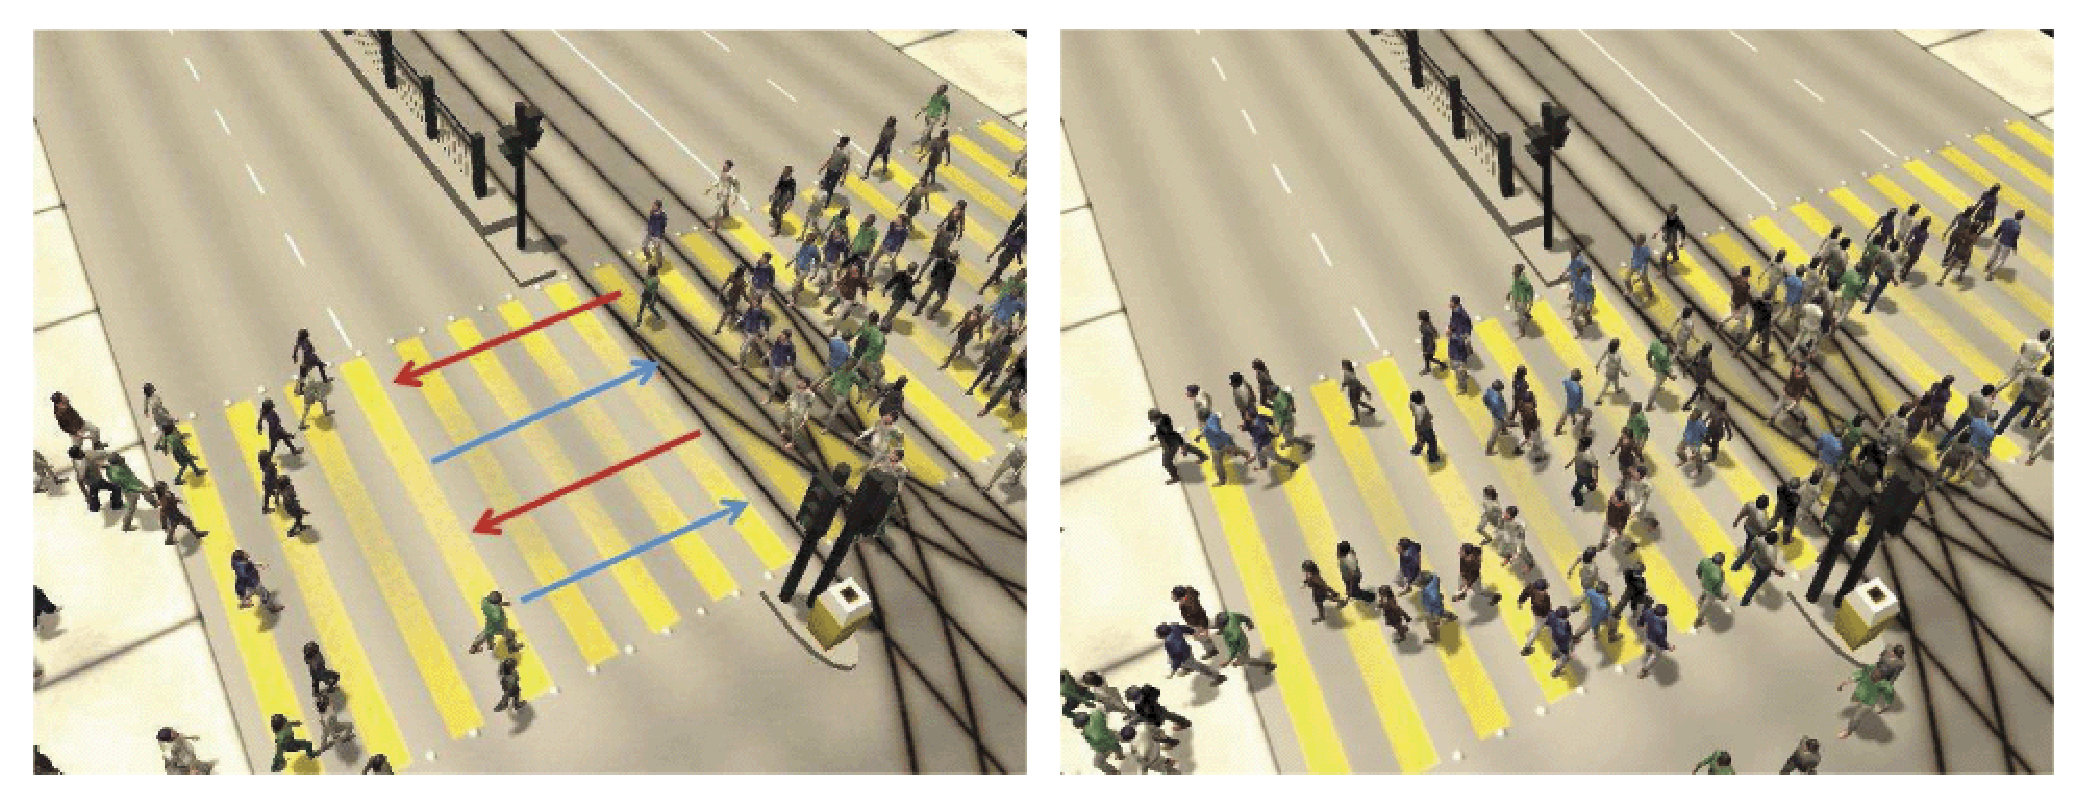
\includegraphics[scale=0.4]{navigation_fields.eps}
  \caption{Motion Planning for Crowd using Navigation Fields \citep{patil}}
  \label{fig:navigation}
\end{figure}

Extending the control vertically, in \citep{musse2} a hierarchical model for real time simulation of virtual human crowds is proposed allowing different control features at levels of crowd, groups or individuals. This is an example of hybrid approach where it is possible to increase the complexity of crowd-group-individual behaviours according to the problem to be simulated.

By means of these techniques, it was visually proven that very convincing and realistic results can be produced. Nevertheless, the identity and the decision capacity of each of the individuals is partially if not completely lost.

\section{Crowd Motion Simulation}

Purely simulation strategies, which is the case of this thesis, discard any pre-planned decision and the final result is entirely based on the global consequences of local interactions of members of the population. This is known as Agent-Based Model or Individual-Based Model. This will be detailed in Chapter \ref{chap:agent-based_model} and for further information check  \citep{red3D}.

The main idea this thesis is settled on is the simple principle stated by C. Reynolds, the pioneer of flocking behaviours, which claimed that very simple rules can arise emergent behaviours without involving any central coordination. Notice again the concept of emerge.

One of the earliest works  in group behaviours was Craig Reynolds' flocking algorithm which was a distributed behaviour model for flocks, herds and schools \citep{reynolds}. The individuals of his flocking system are called ``Boids'' and are subjected to three simple rules: cohesion, alignment and separation.

This classic research not only presents a flocking algorithm, but also marks a turning point proposing an individual virtual force model as the way to affect how each agent move. The approach presented in this thesis has adopted that model.

\begin{figure}[!htb]
  \centering
  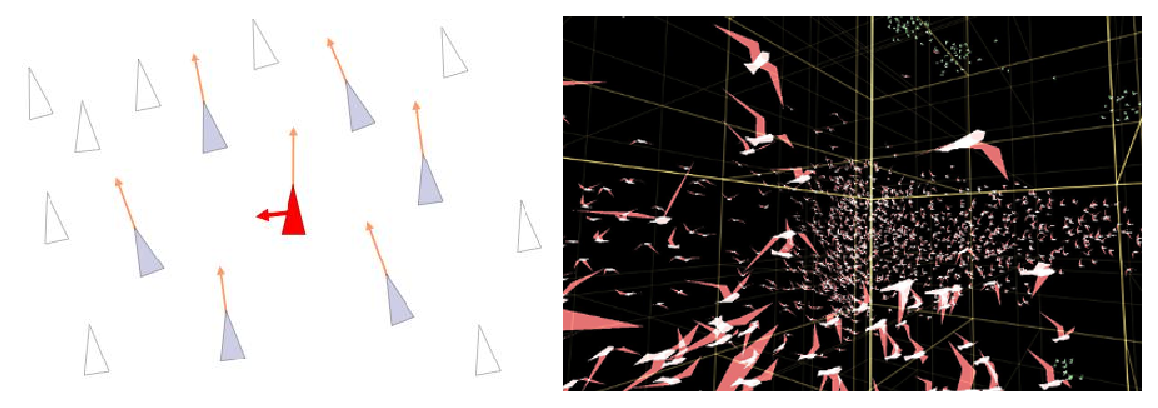
\includegraphics[scale=0.65]{reynolds_flocking.eps}
  \caption{Flocking System following the Virtual Force Model proposed by C. W. Reynolds \citep{reynolds}}
  \label{fig:massive}
\end{figure}

Starting from this robust and solid idea, tons of research paths can be taken in order to acquire and compare different approaches for crowd simulation. For instance, C. Wang \& T. Li suggest an evolving crowd motion simulation \citep{wang}. In that research, the use of genetic algorithms is proposed to generate optimal virtual forces according to the given environment and desired movement behaviour.

Although Craig Reynolds presents a base-approach which models very accurately the way crowds behave in the real world, the main disadvantage is that configuring the forces in order to generate desired motion behaviours remains empirical. And again, we are witnesses of a characteristic inherent to emergent behaviours.

\section{MASSIVE Software}

MASSIVE stands for Multiple Agent Simulation System in Virtual Environment and is a software developed by Stephen Regelous in Weta Digital, as a request from Peter Jackson to recreate those epic battle scenes that Tolkien described in the books of the Lord of the Rings. Massive has contributed to the creation of many awarding visual effects, particularly  the sequences; and due to this, it has been developed into a complete product and has been licensed by many other visual effects houses.

\begin{figure}[!htb]
  \centering
  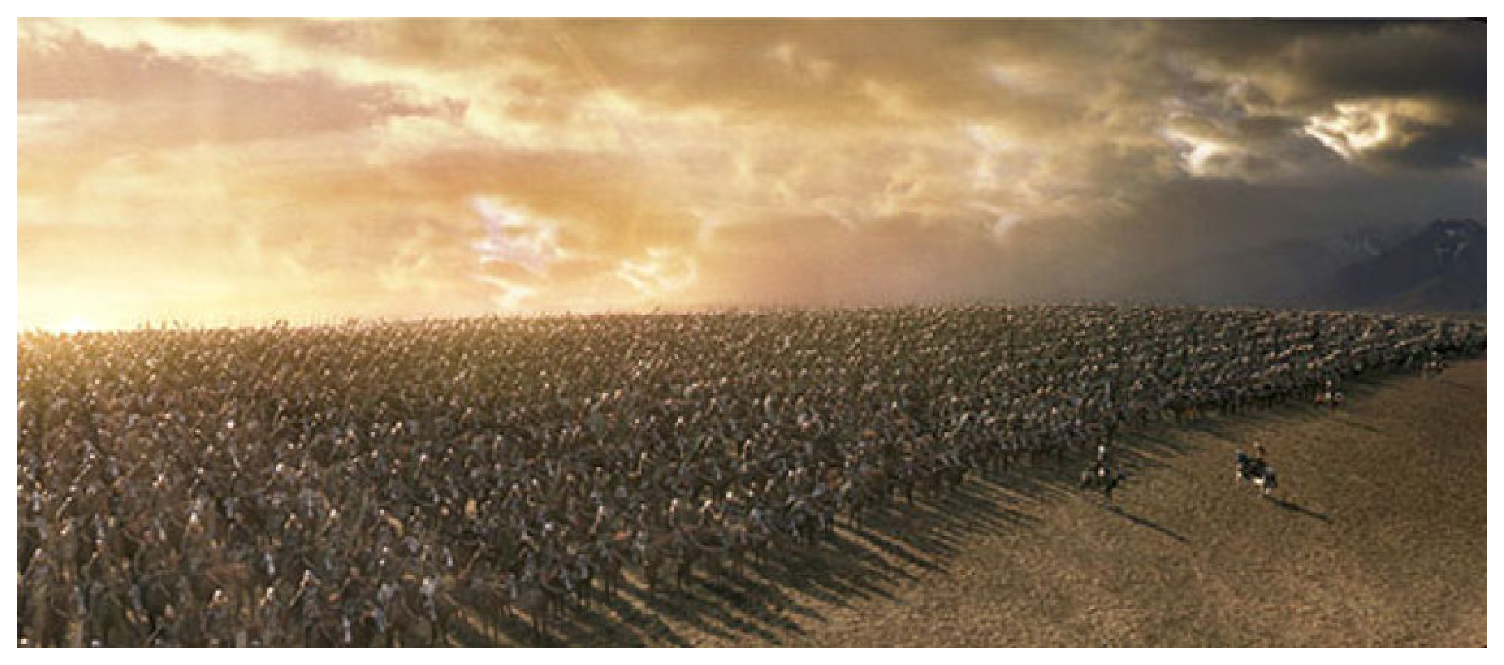
\includegraphics[scale=0.5]{rohan_army.eps}
  \caption{Award winning battle scene from 'The Lord of the Rings: Return of the King'}
  \label{fig:massive}
\end{figure}

Massive introduces a very interesting model approach which consists in treating each agent as a combination of a body and a brain. The body defines the physical characteristic of the agent and the brain is a fuzzy logic network which controls the actions of the agent such as following an arbitrary terrain, avoiding obstacles or interacting with other agents. This thesis has adopted this natural design combined with the flexibility that scripting languages provide.

Each action is associated to a pre-recorded animation, rather obtained from motion captured session or hand-animated, and will be blended between them in order to achieve the movement of the character. Apart from Artificial Intelligence features, it includes other abilities such as Rigid Body Dynamics (RBD), cloth simulation or GPU rendering. 



\ifx\isEmbedded\undefined
% References
\addcontentsline{toc}{chapter}{References}
\bibliographystyle{../ref/harvard}
\bibliography{../ref/master}
\pagebreak
\end{document}
\fi
\ifx\isEmbedded\undefined

\documentclass[12pt]{report}
	
% FONT RELATED
%\usepackage{times} %Move to times font
\usepackage[labelfont=bf,textfont=it]{caption}
\usepackage[utf8]{inputenc}

% LINKS, PAGE OF CONTENT, REF AND CROSS-REF, HEADERS/FOOTERS
\usepackage[hidelinks]{hyperref}
\usepackage{fancyhdr}
\usepackage{acronym}

% FIGURES, GRAPHICS, TABLES
\usepackage{graphicx}
\usepackage{parskip}
%\usepackage{subfigure}
\usepackage{subfig}
\usepackage{wrapfig}
\usepackage{subfloat}

% COLOURS, TEXT AND FORMATTING
\usepackage{array}
\usepackage{color}
\usepackage{setspace}
\usepackage{longtable}
\usepackage{multirow}

% ADVANCED MATHS, PSEUDO-CODE
\usepackage{amsmath}
\usepackage{alltt}
\usepackage{amsfonts}

% ALGORITHMS
\usepackage{algorithm}
\usepackage{algorithmic}

% LANDSCAPE FOR CLASS DIAGRAM
\usepackage{pdflscape}

% BIBLIOGRAPHY
\usepackage[authoryear]{natbib}
\bibpunct{(}{)}{;}{a}{,}{,}

% USE IN DISSER:

\setlength\oddsidemargin{0.85cm}
\setlength\evensidemargin{0.85cm}

\setlength\textheight{21.0cm}
\setlength\textwidth{15.0cm}

% indent at each new paragrapg
\setlength\parindent{0.5cm}

\setlength\topmargin{-0.2in}
\renewcommand{\baselinestretch}{1.3}

%REPORT

%\setlength\oddsidemargin{1cm}
%\setlength\evensidemargin{0.3in}
%%\setlength\headsep{2.5in}
%
%\setlength\textheight{9.0in}
%\setlength\textwidth{5.5in}
%
%% indent at each new paragrapg
%\setlength\parindent{0.5cm}
%
%%\setlength{\parskip}{10.5ex}
%
%\setlength\topmargin{-0.2in}

%\newcommand{\HRule}{\rule{\linewidth}{0.5mm}}
\newcommand{\HRule}{\rule{\linewidth}{0.0mm}}

% Color definitions (RGB model)
\definecolor{ms-comment}{rgb}{0.1, 0.4, 0.1}
\definecolor{ms-question}{rgb}{0.4, 0.0, 0.0}
\definecolor{ms-new}{rgb}{0.2, 0.4, 0.8}


\graphicspath{{../img/}}
\begin{document}
\fi

\chapter{Technical Background}
\label{chap:technical_background}

The background needed for doing research on engineering or any technical discipline is extremely important, and frequently is what makes the difference between a solid, consistent and robust study from a weak one. Many mathematical and physical concepts (specially physical) are critical to understand analytically the ideas, reasoning and logical models presented in this research.

This chapter intends to describe formally the main ground concepts where this thesis is settled on. Although this may only be a brief glimpse of all the ideas applied directly or indirectly, and a much finer conceptual background might be developed, this should be enough for following the approach.

The source consulted to write this section was the chapter A Maths and Physics Primer, in the book Programming Game AI by Example \citep{buckland}.

\section{Physics}

In any research that involves modelling the real world, physical rules will acquire a fundamental role, particularly the ones concerned with motion. Next, the key concepts to understand the virtual force model will be presented.

\begin{itemize}

\item{{\bf Time.} This is a concept that everybody has in mind. Physically speaking, time is a dimension in which events can be ordered from the past through the present into the future. It is a continuous scalar quantity with no direction measured in seconds. Time in computer simulations and computer games might be measured in seconds, like in the real world, or in \emph{virtual seconds} or \emph{ticks}. This will be discussed more in depth in Chapter \ref{chap:application_design_implementation}: Application Design and Implementation.}

\item{{\bf Mass.} It is a scalar quantity measured in grams, and it is the measure of an amount of something. This property is directly linked to how fast bodies change of state. For example, if we imagine two people with the same properties except mass, the one with higher mass will require more time to change from standing to running.}

\item{{\bf Strength.} It is the scalar quantity which defines the physical power a person or animal has. Notice that this property is inherent to an individual and does not have direction, if it had, we would be talking about \emph{force}, concept that will be introduced later. And again, this is related with how fast bodies change of state. The bigger strength, the faster change.}

\item{{\bf Position.} These are the location coordinates of a specific point related to an origin. This is not as simple as it might seem, because bodies have a volume, so which exact position a body has, is a controversial discussion. Normally the centre of mass is used to determine the position, but other points can be used depending on the approach. In order to calculate the movement, we need to know the rate of change of the position, both the magnitude and the direction.}

\item{{\bf Velocity.} This is the vector which defines the rate of change of distance over time. Its standard unit of measurement is $m/s$. Mathematically it can be expressed as follows:}

\begin{equation}
  v=\frac{\Delta x}{\Delta t}
\end{equation}

\item{{\bf Acceleration.} It is a vector which defines the rate of change of velocity over time. Acceleration is written as $m/s^2$, and expressed by:}

\begin{equation}
  a=\frac{\Delta v}{\Delta t}
\end{equation}

\item{{\bf Force.} This is the main element of the physical model followed by this thesis. 
 According to Isaac Newton: ``An impressed force is an action exerted upon a body in order to change its state, either of rest, or of uniform motion in a right line''.
 Therefore, a force is a quality that can alter an object's speed or line of motion. It is measured in Newtons and represented as a vector, with both magnitude and direction}

\end{itemize}

We know that in order to change the position of an object (to move it), it is needed to make its velocity greater than 0, and to achieve that, there has to exist an acceleration. Basically, what the object is experimenting is a change of state due to an acceleration produced by forces.

Newton's second law states the relatioship between an object's mass $m$, its acceleration $a$, and the applied force $F$ by the equation:

\begin{equation}
  F=ma
\end{equation}

%\newpage
Therefore, this gives us the key to perform a physically based simulation. According to everything mentioned before, the motion an object experiments in a physically based virtual world can be calculated after synthesizing all the forces applied over it:

\begin{enumerate}
%\centering
\item $a = \frac{F_{total}}{m}$
\item $v_{t+1} = v_{t}+a$
\item $p_{t+1} = p_{t}+v_{t+1}$
\end{enumerate}

\section{Reynold's Flocking Algorithm}

Craig W. Reynolds proposed in 1987 a model to simulate natural group behaviours such as herds, flocks or schools \citep{reynolds}. This is a very powerful mechanism to use in crowds, besides sharing the principles this thesis is based on. The method works by applying three simple rules to each individual of the flock, which Reynolds called \emph{boids}, that make them move as a unit.

\begin{figure}[!h]
  \centering
  \begin{tabular}{c c c}
  	\subfloat[Cohesion Rule]{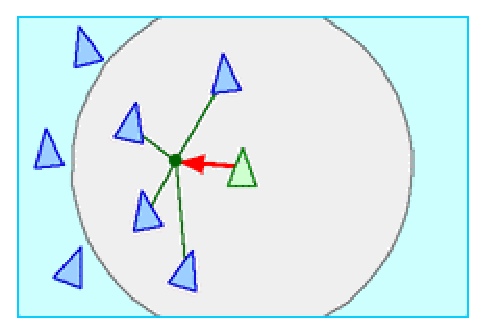
\includegraphics[scale=0.6]{cohesion.eps}} &
 	\subfloat[Separation Rule]{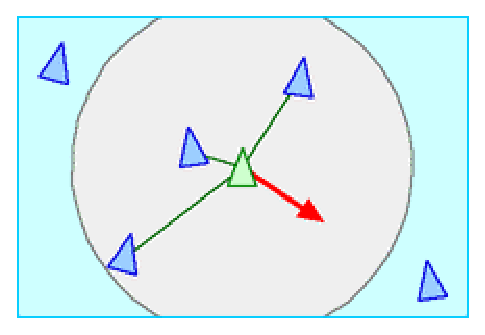
\includegraphics[scale=0.6]{separation.eps}} &
  	\subfloat[Alignment Rule]{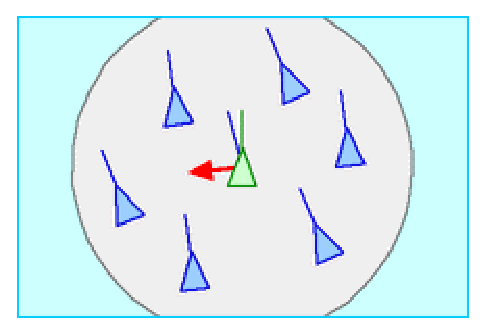
\includegraphics[scale=0.6]{alignment.eps}} \\
 \end{tabular}
  \caption{Reynolds' Model Rules}
  \label{fig:crowds}
\end{figure}

Each boid knows a set of neighbours in the flock which influences its movement. Only the ones that are within a certain distance are considered neighbours, and the rest are ignored; thus, boids have local conscience of the flock. According to the virtual force model, those simple rules produce these three steering forces:

\begin{itemize}

\item{{\bf Cohesion.} This force makes the boid to move towards the centre of mass of the neighbourhood so that they remain close to each other.\\

Let $p$ be the position and $v$ the velocity of the current boid, $p_i$ the position of the neighbour i and $n$ the number of neighbours:

\begin{equation}
  centreOfMass=\frac{\sum_{i=1}^np_i}{n}
\end{equation}

\begin{equation}
  cohesionForce=normalize(centreOfMass-p)-normalize(v)
\end{equation}
}

\item{{\bf Separation.} This force makes the boid to move away from its neighbours, to avoid remaining too close.\\

Let $p$ be the position of the current boid, $p_i$ the position of the neighbour i, $d_i$ the distance to the neighbour i and $n$ the number of neighbours:

\begin{equation}
  separationForce=\sum_{i=1}^n\frac{normalize(p-p_i)}{d_i}
\end{equation}
}

\item{{\bf Alignment.} This attemps to keep the boid aligned with their neighbours.\\

Let $p$ be the position and $v$ the velocity of the current boid, $p_i$ the position and $v_i$ the velocity of the neighbour i and $n$ the number of neighbours:

\begin{equation}
  averageHeading=\frac{\sum_{i=1}^nnormalize(v_i)}{n}
\end{equation}

\begin{equation}
  alignmentForce=averageHeading-normalize(v)
\end{equation}
}

\end{itemize}

\section{Finite State Machine (FSM)}

Finite State Machines, or FSM, have been the main instrument of choice to imbue an agent the illusion on intelligence. Some of the reasons are these:

\begin{itemize}
\item{Quick and simple to code}
\item{Easy to debug}
\item{Little computational overhead}
\item{They are intuitive}
\item{They are flexible}
\end{itemize}

Historically, a FSM is a rigidly formalized device used by mathematicians to solve problems, whose precursor might be considered the Turing Machine. The idea is to decompose an object's behaviour into easily manageable ``chunks'' or states. For instance, a light switch is a very simple FSM where \emph{off} and \emph{on} are the states. Transitions are made by the input of the fingers. By clicking the switch up it triggers the transition from off to on, and by clicking the switch down it triggers the transition from on to off. There is no action associated with the off state, but when it is on, the electricity is allowed to flow and light up the room.

\begin{figure}[!htb]
  \centering
  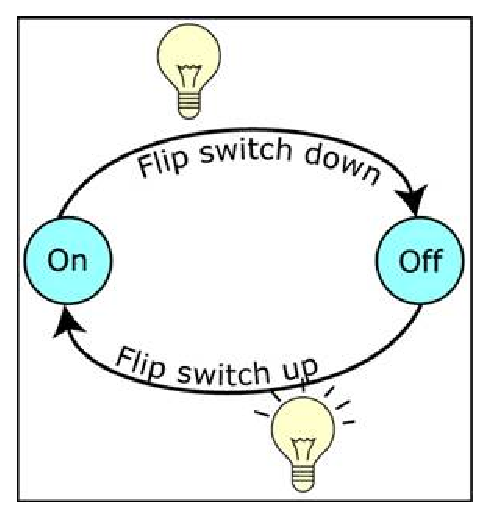
\includegraphics[scale=0.6]{fsm.eps}
  \caption{Light Finite State Machine}
  \label{fig:light}
\end{figure}

As mentioned above, one of the main advantages of FSM is that they are very intuitive. It is human nature to think about things as being in one state or another. Humans do not really work like FSM but sometimes it is useful to think our behaviour in this way. It is fairly easy to break down an agent's behaviour into a number of states with associated actions and to create rules to transit among them.

One feature that notably enhance the power of FSM and allow intercommunication among agents is the message passing support. Intelligent agents can send and receive information to each other, and act upon it. This is a model which reflects quite accurately how real interactions work. This messages are sent in the form of packets of data to other agents, which might influence their behaviour triggering a transition to a different state. If an archer sends an ``arrow'' message to an enemy, this might respond changing his state from alive to dead.

\ifx\isEmbedded\undefined
% References
\addcontentsline{toc}{chapter}{References}
\bibliographystyle{../ref/harvard}
\bibliography{../ref/master}
\pagebreak
\end{document}
\fi
\ifx\isEmbedded\undefined

\documentclass[12pt]{report}
	
% FONT RELATED
%\usepackage{times} %Move to times font
\usepackage[labelfont=bf,textfont=it]{caption}
\usepackage[utf8]{inputenc}

% LINKS, PAGE OF CONTENT, REF AND CROSS-REF, HEADERS/FOOTERS
\usepackage[hidelinks]{hyperref}
\usepackage{fancyhdr}
\usepackage{acronym}

% FIGURES, GRAPHICS, TABLES
\usepackage{graphicx}
\usepackage{parskip}
%\usepackage{subfigure}
\usepackage{subfig}
\usepackage{wrapfig}
\usepackage{subfloat}

% COLOURS, TEXT AND FORMATTING
\usepackage{array}
\usepackage{color}
\usepackage{setspace}
\usepackage{longtable}
\usepackage{multirow}

% ADVANCED MATHS, PSEUDO-CODE
\usepackage{amsmath}
\usepackage{alltt}
\usepackage{amsfonts}

% ALGORITHMS
\usepackage{algorithm}
\usepackage{algorithmic}

% LANDSCAPE FOR CLASS DIAGRAM
\usepackage{pdflscape}

% BIBLIOGRAPHY
\usepackage[authoryear]{natbib}
\bibpunct{(}{)}{;}{a}{,}{,}

% USE IN DISSER:

\setlength\oddsidemargin{0.85cm}
\setlength\evensidemargin{0.85cm}

\setlength\textheight{21.0cm}
\setlength\textwidth{15.0cm}

% indent at each new paragrapg
\setlength\parindent{0.5cm}

\setlength\topmargin{-0.2in}
\renewcommand{\baselinestretch}{1.3}

%REPORT

%\setlength\oddsidemargin{1cm}
%\setlength\evensidemargin{0.3in}
%%\setlength\headsep{2.5in}
%
%\setlength\textheight{9.0in}
%\setlength\textwidth{5.5in}
%
%% indent at each new paragrapg
%\setlength\parindent{0.5cm}
%
%%\setlength{\parskip}{10.5ex}
%
%\setlength\topmargin{-0.2in}

%\newcommand{\HRule}{\rule{\linewidth}{0.5mm}}
\newcommand{\HRule}{\rule{\linewidth}{0.0mm}}

% Color definitions (RGB model)
\definecolor{ms-comment}{rgb}{0.1, 0.4, 0.1}
\definecolor{ms-question}{rgb}{0.4, 0.0, 0.0}
\definecolor{ms-new}{rgb}{0.2, 0.4, 0.8}


\graphicspath{{../img/}}
\begin{document}
\fi

\chapter{Agent-Based Model}
\label{chap:agent-based model}

After an introductory chapter and a background overview, this is where this document starts dealing with the particular approach studied in this thesis. The solution will be presented following a bottom-up explanation line, since the author believes that it will be clearer for the reader and is the way behaviours emerge. Thus, in this chapter the abstract model for an individual which belongs to a crowd, and which lives in the virtual world, is explained into details. This individual, which will be referred as \emph{agent} from now on, is the element that will encapsulate the intelligence of the system. Therefore, this approach is based on individual intelligent agents rather than any global mechanism, from whose interactions a group behaviour will arise. As stated before, the crowd behaviour will have as much quality as the agent behaviours have.

Next Chapter will take a wider vision presenting the concept of crowd and the world which holds the complete simulation.

``An agent autonomous agent is a system situated within and a part of an environment that senses that environment and acts on it, over time, in pursuit of its own agenda and so as to effect what it senses in the future'' \cite{buckland}

Since the old Greece, some philosophers argued about a spiritual division between soul and body, other scientists consider the ability of thinking something that escapes the bounds of the physical body. Without going such further, this thesis presents an abstract agent model divided in two parts: a body and a brain.

\section{Agent Body}

This part is the one which is materially in the world, and there is no intelligence in here. It is completely physically based and most of its attributes are immutable during a simulation. The body represents how big an agent is, or how fast it is, etc. This way, an agent might be big and slow or small and fast. These attributes might even limit the capacity of decision of the thinking partition of the agent. Let us imagine a situation where a prey's brain desperately keeps requesting for increasing the velocity to escape from a predator, but the body cannot perform a higher speed. Next, the list of the physical properties which define the body of an agent are presented.

\subsection{Physical Properties}

\begin{itemize}

\item{{\bf Mass.} The mass of an agent determines how much acceleration a force produces on it.
Taking the assumption that agents have comparable densities, it is also employed to visualize their size}

\item{{\bf Strength.} This will influence in the \emph{prime mover force}, which is the force an agent applies on itself to move in the space. Therefore, having agents with the same mass, the strong ones will have the ability of opposing to external forces easily or to produce more self-acceleration, changing their velocity faster. The strength might vary if, for example, the agent gets tired or receives any sort of damage.}

\item{{\bf Maximum Strength.} This is the amount of strength that an agent has when it is fully recovered.}

\item{{\bf Velocity.} This is the current velocity that an agent possesses and, contrary to the strength, this attribute has both magnitude and direction. This is the rate of change of the agent's location; thus, it is used to obtain the next position. It is calculated with the acceleration that the total force produce on the agent.}

\item{{\bf Maximum Speed.} This is the higher punctual speed that an agent can move in the world with. Do not confuse this with how fast an agent can change of physical state, which is related with forces and mass (acceleration). Consider the next example: a cheetah can change from 0 to 100 km/h in a matter of seconds (high acceleration); on the other hand, a high-speed train, which needs a lot of force (strength with direction) to move such a big mass, has much smaller acceleration, but it can travel at 200 km/h (high maximum speed).}

\item{{\bf Vision Radius.} This property determines which portion of the world the agent is aware of. This is mainly used to calculate the other agents that one agent can perceive, which will conform its neighbourhood. Therefore, an explorer may have a large vision radius, meanwhile a blind agent will have vision radius 0, and will need to receive information about the world by other means, such as somebody whispering at its ear (message passing).}

\end{itemize}

\begin{figure}[!htb]
  \centering
  \includegraphics[scale=0.3]{agent.eps}
  \caption{One single agent with its physical properties}
  \label{fig:navigation}
\end{figure}

At this point, a comment regarding to the development of this method might be pertinent. How an agent's body behaves in the virtual world is uniquely ruled by physical laws. The brain might say ``move up'' and apply a force towards the sky but if this force is smaller than the gravity, then the agent will descend. Hence, the piece of this system relative to the physical simulation or the physical properties of an agent is something static, a fixed and solid structure which works. That is why it is implemented in a compiled language. Nevertheless, somebody's way of thinking or acting, might be so diverse that it needs a flexibility that a compiled language cannot provide.\footnote{Although the design and implementation of the approach are treated in chapter \ref{chap:application_design_implementation}, the author believes that it is convenient to mention some implementations details which are important to understand how much flexibility or scalability this approach offers.}

\section{Agent Brain}
This is where resides the ``intelligence'' of the agent. This piece has the responsability of determining which motion an agent describes, how to interact with the world and how to interact with other agents.

The main mechanism used to model a brain is a FSM, although any other device might be used such as an artificial neural network, which is the closer to reality. This computational box receives a set of information both from the body and from the environment. This includes the physical properties, the current state of the agent, a table of own attributes, a list with its neighbours and their information and a list of the incoming messages. After processing, the brain will communicate to the body what to do by returning certain parameters.

\begin{itemize}

\item{{\bf Prime Mover Force.} This is the instruction the brain sends to the body in order to perform a specific displacement. This will be explained into details in the next chapter during the section of forces, but it is basically the force that the muscles should apply on the body to move it in a certain direction and with certain acceleration. The direction is a free choice, but the magnitude should be influenced by the current strength to acquire a realistic motion}

\item{{\bf Heading.} The brain can set the heading of the agent too; this is normally established by the velocity, but there are some kind of motions, such as lateral movements, where the heading does not point in the same direction than the velocity.}

\item{{\bf Strength.} According to this model, it is the brain who decides how much strength the actions of the agent consume or, by the contrary, how fast it recovers. So the new strength is returned.}

\item{{\bf State.} The brain will tell to the body the new state, which might be the old one, or a new one if some transition was triggered.}

\item{{\bf Messages.} A list with the messages to send to the agent's neighbours. This messages have certain type of information detailed later, and if the receiver knows how to react upon it, its behaviour may be affected}

\end{itemize}

This is where the usability and beauty of the approach arises. The behaviours are script based; therefore, having all the gears of the system spinning properly, any new brain can be added at any time. For the behaviours proposed, it was chosen to use a FSM, as a simple and effective mechanism, but any other more sofisticated method could be used. Different techniques such as movement prediction, statistical study, evolving algorithms, etc. might be employed for developing new agent behaviours and observe the emergent configuration of the crowd.

\subsection{Capacity of Decision}

This is what, under a physical consistency, drives the simulation. The ability that an agent has to take decisions is the main input to produce a simulation. If we have in mind any simple video game in where we control a character to interact with a world, we are taking decisions, tons of them. They might be long term ones (reach a target) or short term ones (this way seems a shortcut). Thus, the idea is automate this task. An infinite amount of things might influence every decision we take in real life: in which state we feel, where we are, how tired we are, which is our physical shape, who is surrounding us, what we know about who is surrounding us, etc. In order to take accurate decisions a large amount of information needs to be taken into account, besides all the different possibilities available; that could produce extremely complex FSM's or other artifacts very difficult to handle.

\subsection{The Illusion of Intelligence}

Intelligence is a very complex concept. It is thought as a mental capability that involves things such as the ability to reason, plan, solve problems, think abstractly, comprehend complex ideas, learn quickly or learn from experience.

The \emph{Artificial Intelligence} (AI) is the science which studies and develops intelligent machines and software. The general problem of simulating (or creating) intelligence has been broken down into a number of specific sub-problems related to the tasks mentioned in the previous paragraph. There is no established unifying theory or paradigm that guides AI research. Researchers disagree about many issues.

As a general rule, it can be considered that the decisions an agent takes and behaviour it presents will tell us if it is intelligent or not. Building a simple behaviour is a matter of minutes, building a very intelligent behaviour might require several times the time this thesis was done in.


\section{Interaction among agents. Message passing}

The other important feature essential for an authentic emergent group behaviour is how the individuals are interconnected, as stated in \citep{kleinrock}. This is acheived by passing messages, which allows communication among the agents.

A message is a package which contains information that includes:

\begin{itemize}

\item{{\bf Agent Identification.} This is used to recognize the sender of the message.}

\item{{\bf Label.} This is the string of text which contains the information inherent to the message. A message might have any type of label, meanwhile the behaviour designer provides the mechanisms to handle it. It might be from an ``attack'' message to a ``shall we dance?'' message.}

\item{{\bf Position.} The position of the sender. Take into account that having the agent identification, we can check all the information about it looking into the neighbours. But it might happen, that the sender is out of our vision radius. Imagine that we hear a far shout, the only we know about it is what it says and where it comes from.}

\item{{\bf Strength} The strength of the sender. This is use for practical purposes. Knowing the strength of the sender allows to take richer decisions at the time of handle it. For instance, if an ``attack'' arrives to us, we know the strength associated to it; or if a strong warrior sends a ``follow'' message in a battlefield, it may be a wise choice to pay attention to him.}

\end{itemize}

\section{Overview of Possible Behaviours}

A behaviour is the range of actions and mannerisms made by organisms, systems, or artificial entities in conjunction with their environment, which includes the other systems or organisms around as well as the physical environment.

Many of some basic behaviours, which are thought as standard ones in the field of AI, were used directly or inderectly to develop some test behaviours for this thesis. The most classic one is the steering behaviour of the seek which directs the agent to a target position.

\begin{figure}[!h]
  \centering
  \begin{tabular}{c    c}
  	\subfloat[Calculating vector force]{\label{fig:f1}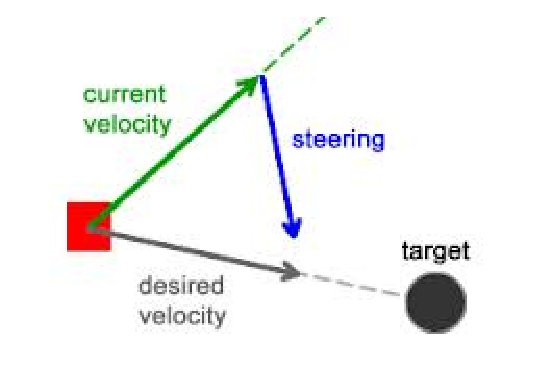
\includegraphics[scale=0.6]{seek_01.eps}} &
 	\subfloat[Shown behaviour]{\label{fig:f2}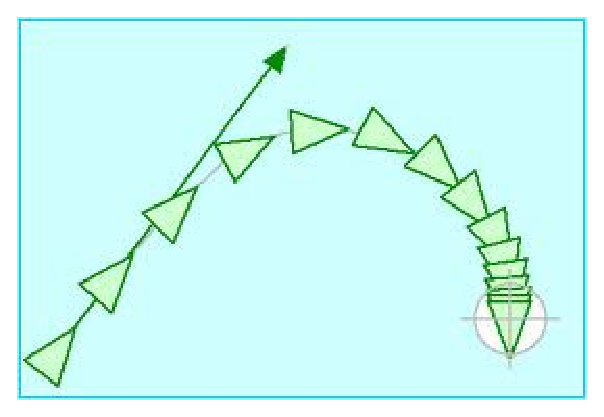
\includegraphics[scale=0.6]{seek_02.eps}} \\
 \end{tabular}
  \caption{Seek Steering Behaviour}
  \label{fig:crowds}
\end{figure}

Let $pos$ be the position, $velocity$ the velocity, and $maxSpeed$ the maximum speed of the agent; and $targetPos$ the position of the target:

\begin{equation}
	desiredVelocity=normalize(targetPos-pos)maxSpeed 
\end{equation}

\begin{equation}
	seekForce=desiredVelocity-velocity 
\end{equation}

This is one example among many other simple behaviours such as flee, arrive, pursuit, evade or wander \citep{buckland}. 

For this approach, more complex and varied behaviours which might involve the previous ones were developed. The method employed was basically logical reasoning and empirical testing, manipulating the motion by means of the prime mover force, besides heading, state, strength and all the other features that the brain supports.

In this way, we might have simple boids that essentially follow the rules of Reynolds' flocking algorithm, or more sophisticated ones. Droids that stand at a certain distance to the target to shot, warriors that send attacks to each others where the strong ones have more chances to reach the victory, dancers that employ forces softly to describe harmonious swings in couples, and more. The testing results will be exposed in further details in Chapter \ref{chap:applications_and_results}: Applications and Results.

\ifx\isEmbedded\undefined
% References
\addcontentsline{toc}{chapter}{References}
\bibliographystyle{../ref/harvard}
\bibliography{../ref/master}
\pagebreak
\end{document}
\fi
\input{chap/crowd_engine}
\ifx\isEmbedded\undefined

\documentclass[12pt]{report}
	
% FONT RELATED
%\usepackage{times} %Move to times font
\usepackage[labelfont=bf,textfont=it]{caption}
\usepackage[utf8]{inputenc}

% LINKS, PAGE OF CONTENT, REF AND CROSS-REF, HEADERS/FOOTERS
\usepackage[hidelinks]{hyperref}
\usepackage{fancyhdr}
\usepackage{acronym}

% FIGURES, GRAPHICS, TABLES
\usepackage{graphicx}
\usepackage{parskip}
%\usepackage{subfigure}
\usepackage{subfig}
\usepackage{wrapfig}
\usepackage{subfloat}

% COLOURS, TEXT AND FORMATTING
\usepackage{array}
\usepackage{color}
\usepackage{setspace}
\usepackage{longtable}
\usepackage{multirow}

% ADVANCED MATHS, PSEUDO-CODE
\usepackage{amsmath}
\usepackage{alltt}
\usepackage{amsfonts}

% ALGORITHMS
\usepackage{algorithm}
\usepackage{algorithmic}

% LANDSCAPE FOR CLASS DIAGRAM
\usepackage{pdflscape}

% BIBLIOGRAPHY
\usepackage[authoryear]{natbib}
\bibpunct{(}{)}{;}{a}{,}{,}

% USE IN DISSER:

\setlength\oddsidemargin{0.85cm}
\setlength\evensidemargin{0.85cm}

\setlength\textheight{21.0cm}
\setlength\textwidth{15.0cm}

% indent at each new paragrapg
\setlength\parindent{0.5cm}

\setlength\topmargin{-0.2in}
\renewcommand{\baselinestretch}{1.3}

%REPORT

%\setlength\oddsidemargin{1cm}
%\setlength\evensidemargin{0.3in}
%%\setlength\headsep{2.5in}
%
%\setlength\textheight{9.0in}
%\setlength\textwidth{5.5in}
%
%% indent at each new paragrapg
%\setlength\parindent{0.5cm}
%
%%\setlength{\parskip}{10.5ex}
%
%\setlength\topmargin{-0.2in}

%\newcommand{\HRule}{\rule{\linewidth}{0.5mm}}
\newcommand{\HRule}{\rule{\linewidth}{0.0mm}}

% Color definitions (RGB model)
\definecolor{ms-comment}{rgb}{0.1, 0.4, 0.1}
\definecolor{ms-question}{rgb}{0.4, 0.0, 0.0}
\definecolor{ms-new}{rgb}{0.2, 0.4, 0.8}


\graphicspath{{../img/}}
\begin{document}
\fi

\chapter{Applications and Results}
\label{chap:applications_results}

\section{Possible real production pipeline}

This chapter has much relevance since it exposes all the different behaviours scripted in order to test the core and perform a set of simulations. But before doing that, it is proposed a real pipeline where this thesis may fit in, proving that this approach might contribute both to the game and VFX industry.

\begin{figure}[!htb]
  \centering
  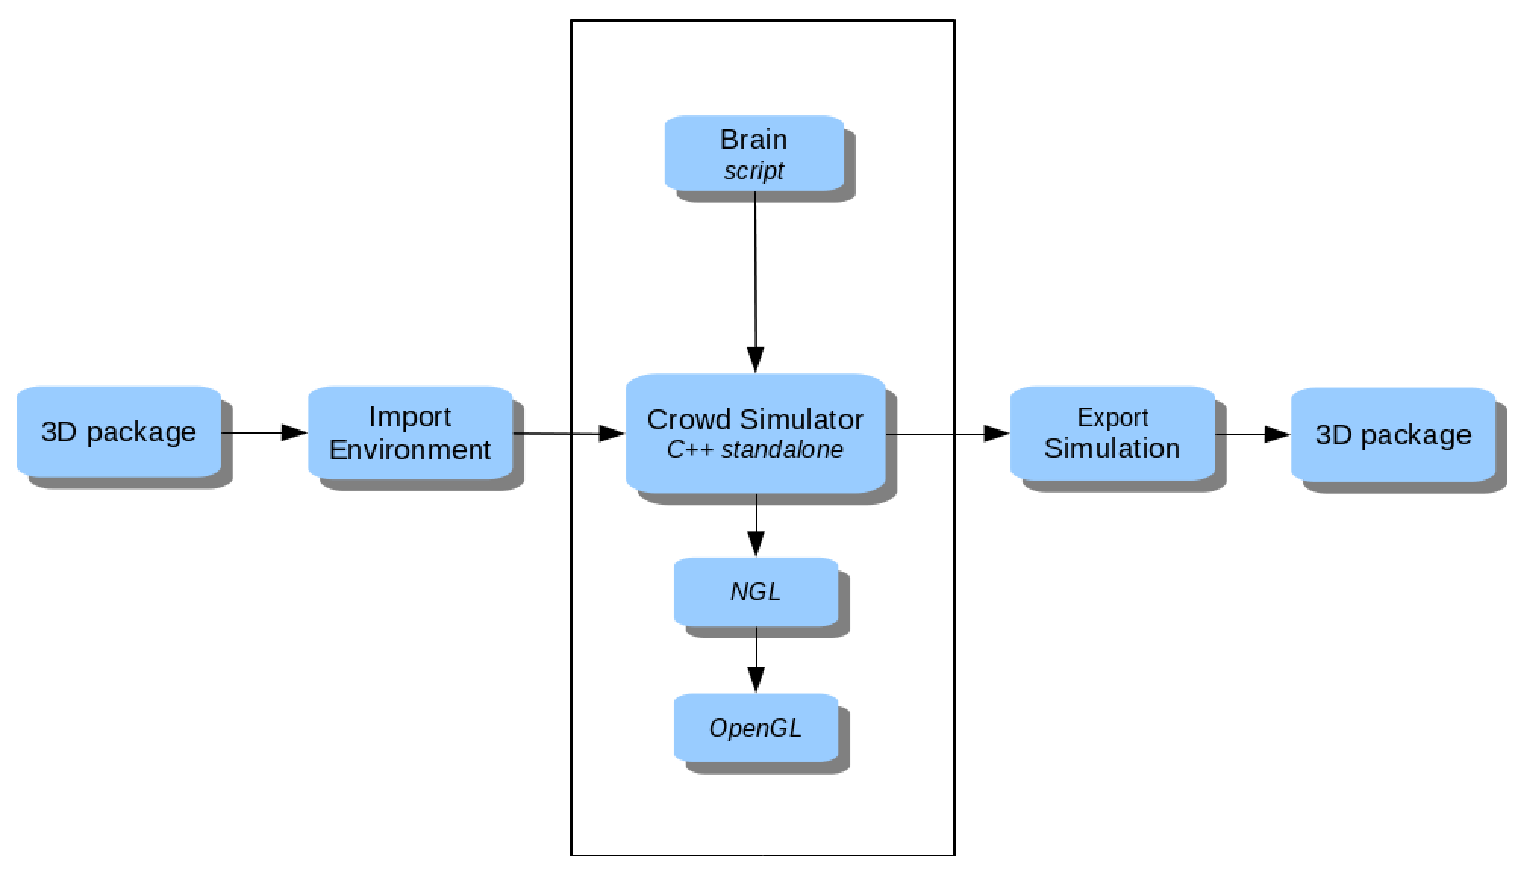
\includegraphics[scale=0.5]{pipeline.eps}
  \caption{Possible pipeline}
  \label{fig:classDiag}
\end{figure}

Any simulation takes place inside a specific environment, therefore it should be possible to import it from a 3D package. When developing this approach, the priorities were behaviours and AI, hence this was left on a second plane. Adding a specific terrain would allow to achieve concrete sequences where a crowd with a particular behaviour is involved.

In order to allow to the engine handle the environment, as well as complex meshes for the agents, it would be needed an efficient physics engine able to produce an accurate collision detection. 

Besides of the previous features, the strength of this approach resides in the flexibility of the behaviours. A script-based brain for a new type of agent can be written, modified and added at any time, and the limitations of a behaviour are only set by the behaviours writer. So a tool based on this approach could be used for any sort of sequence.

The simulation might be performed in a user-assisted way, this means that the user could adjust the different parameters that will modify the simulation. The final behaviour emerges from the individual behaviours and their interconnections (this what this thesis is all about), but as mentioned in the previous chapter, there are physical properties of the virtual world which may lead the simulation in one direction or another.

As final step, the simulation may be exported for finer manipulation and some animations might be attached to the each one of the states of the agents.

Another alternative pipeline might be directly build a plugin that can be loaded at runtime by a 3D full package such as Maya or Houdini.

It is worthy to mention that this thesis describes an approach; a robust and solid base where a very flexible, high quality and productive application can be settle on.

\section{Test Behaviours}

Some behaviours were scripted, in this case in Lua, which is the language chosen for this specific implementation. The behaviours are presented following a structure. First the individual behaviours are explained, in company of the FSM's used for their development if there are, and next the emergent behaviours observed are described.

Notice that for the simulations some different dummies are used. They are just that, dummies to make the visualization more friendly and to provide some intuitive clues about the agent's behaviour. The simulation is about points,transformations and states; and the group behaviour that emerge.

All the videos are available in online platforms or in the master's thesis submission directory.

\subsection{Crowds}

The first test is very basic. The brain of this agents implements the basic behaviour of a flock described by Reynolds \citep{reynolds}. Here, the boids move on the ground as group of flocks kept in union by the three basic rules. So having different flocks interacting in the same region, it is possible to distinguish if a boid belongs to one flock or another. The behaviour emerged here is similiar to the one achieved when used field of forces of navigational mechanisms.

Many different situations might arise when there is contact among several flocks. They might adjust their directions to converge in one big mass of people, they might move parallel in opposite directions, they might diverge, etc.

\begin{figure}[!h]
  \centering
  \begin{tabular}{c c}
  	\subfloat[Random crowd]{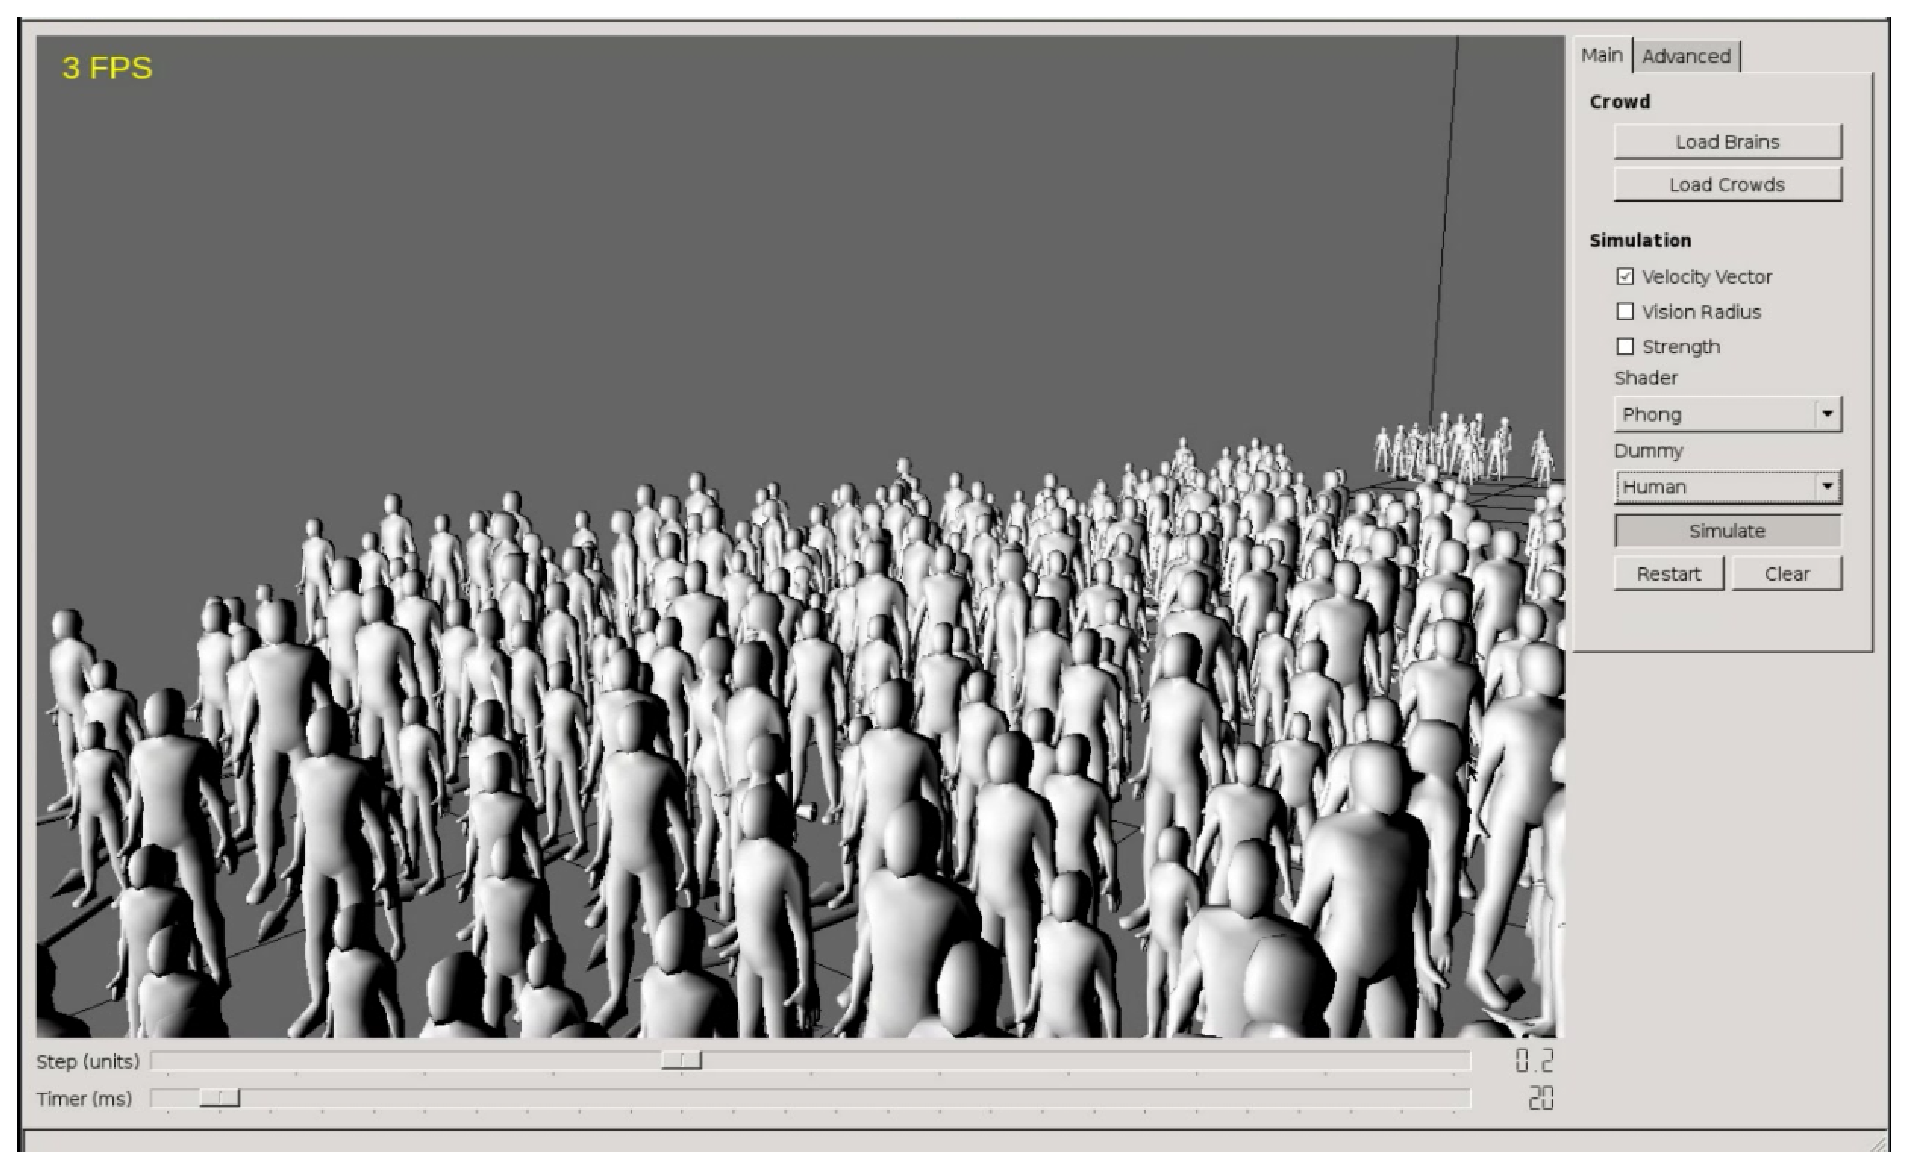
\includegraphics[scale=0.23]{crowds_01.eps}} &
 	\subfloat[Diverging crowd]{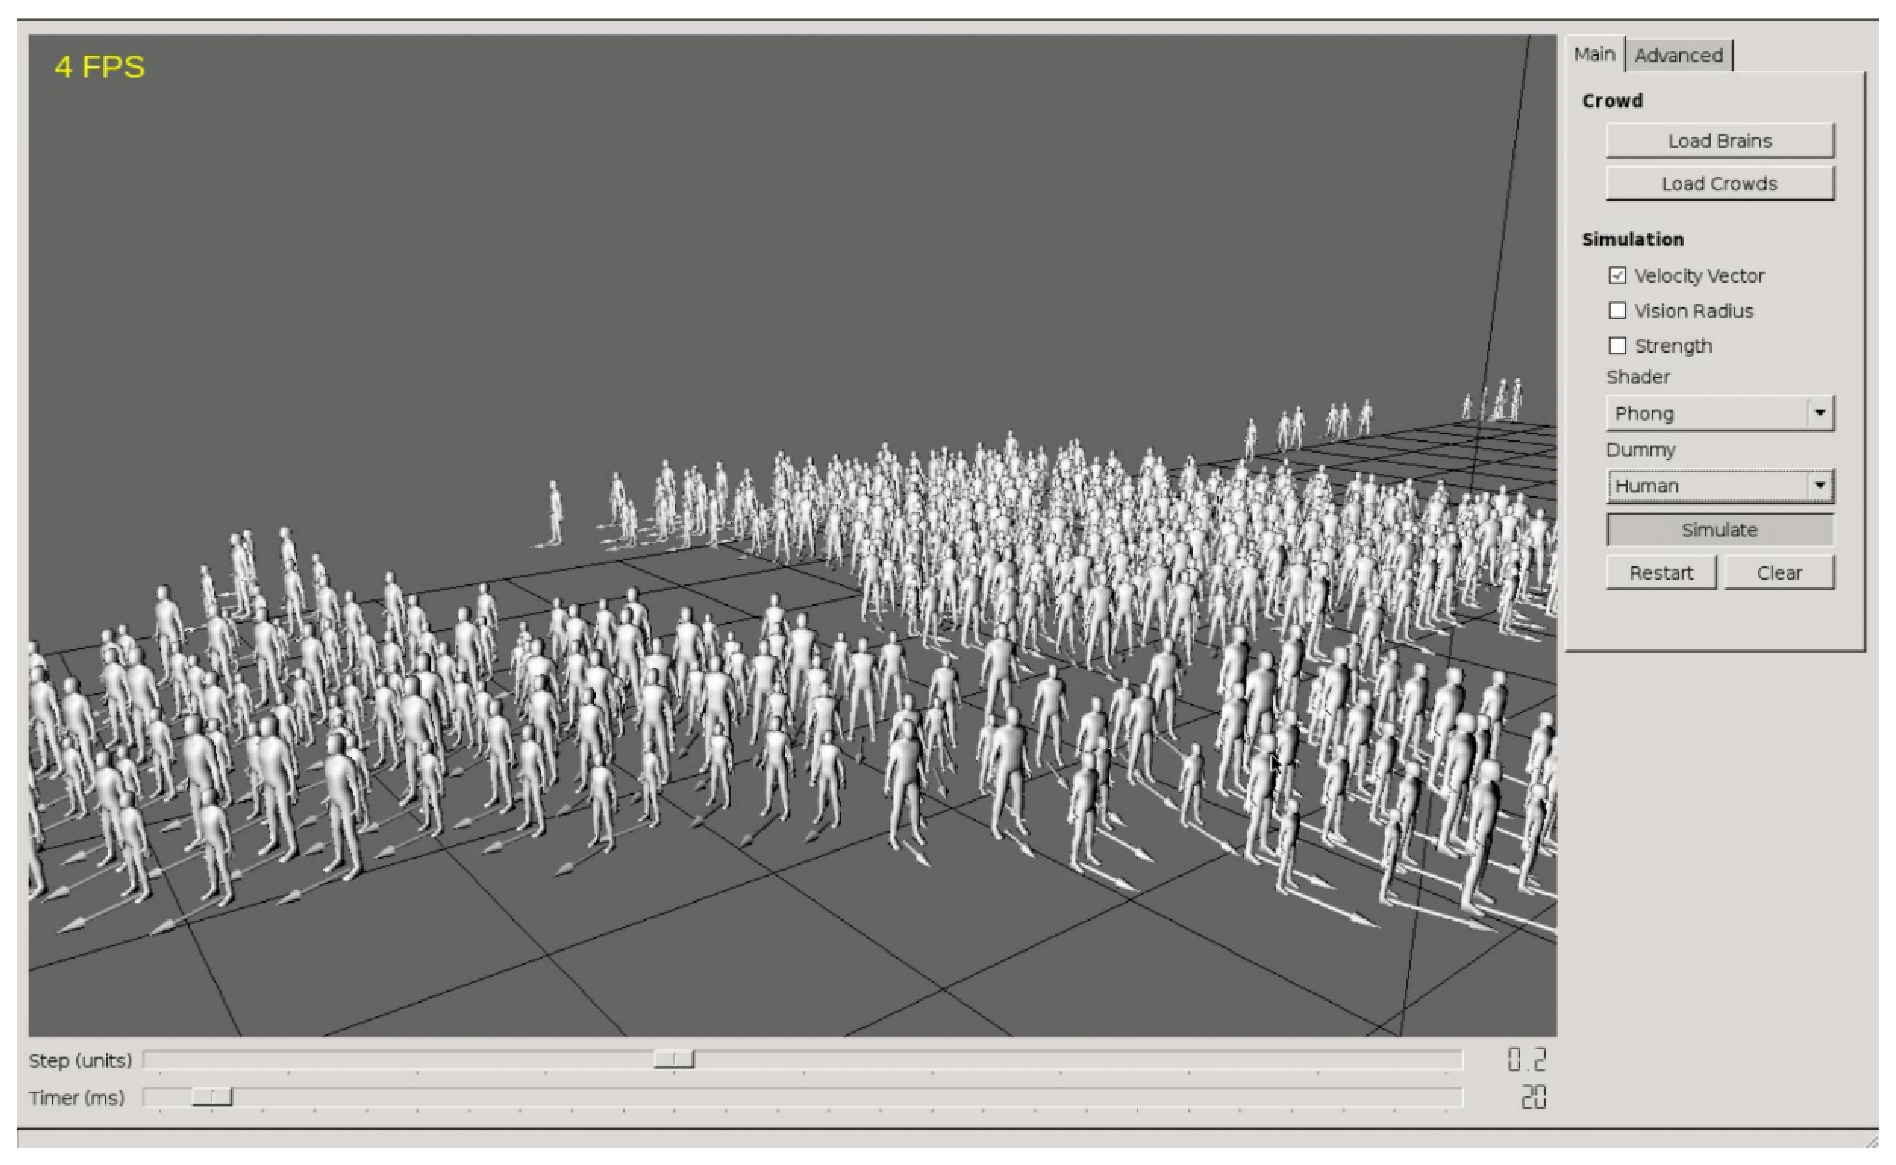
\includegraphics[scale=0.23]{crowds_02.eps}} \\
 \end{tabular}
  \caption{Crowd Simulation}
  \label{fig:crowdsCaptures}
\end{figure}

\newpage
\subsection{Droid Wars}

This behaviour is a little more complex than the previous one. The brain reproduces how a \emph{shooter battle droid} acts. 

\begin{figure}[!h]
  \centering
 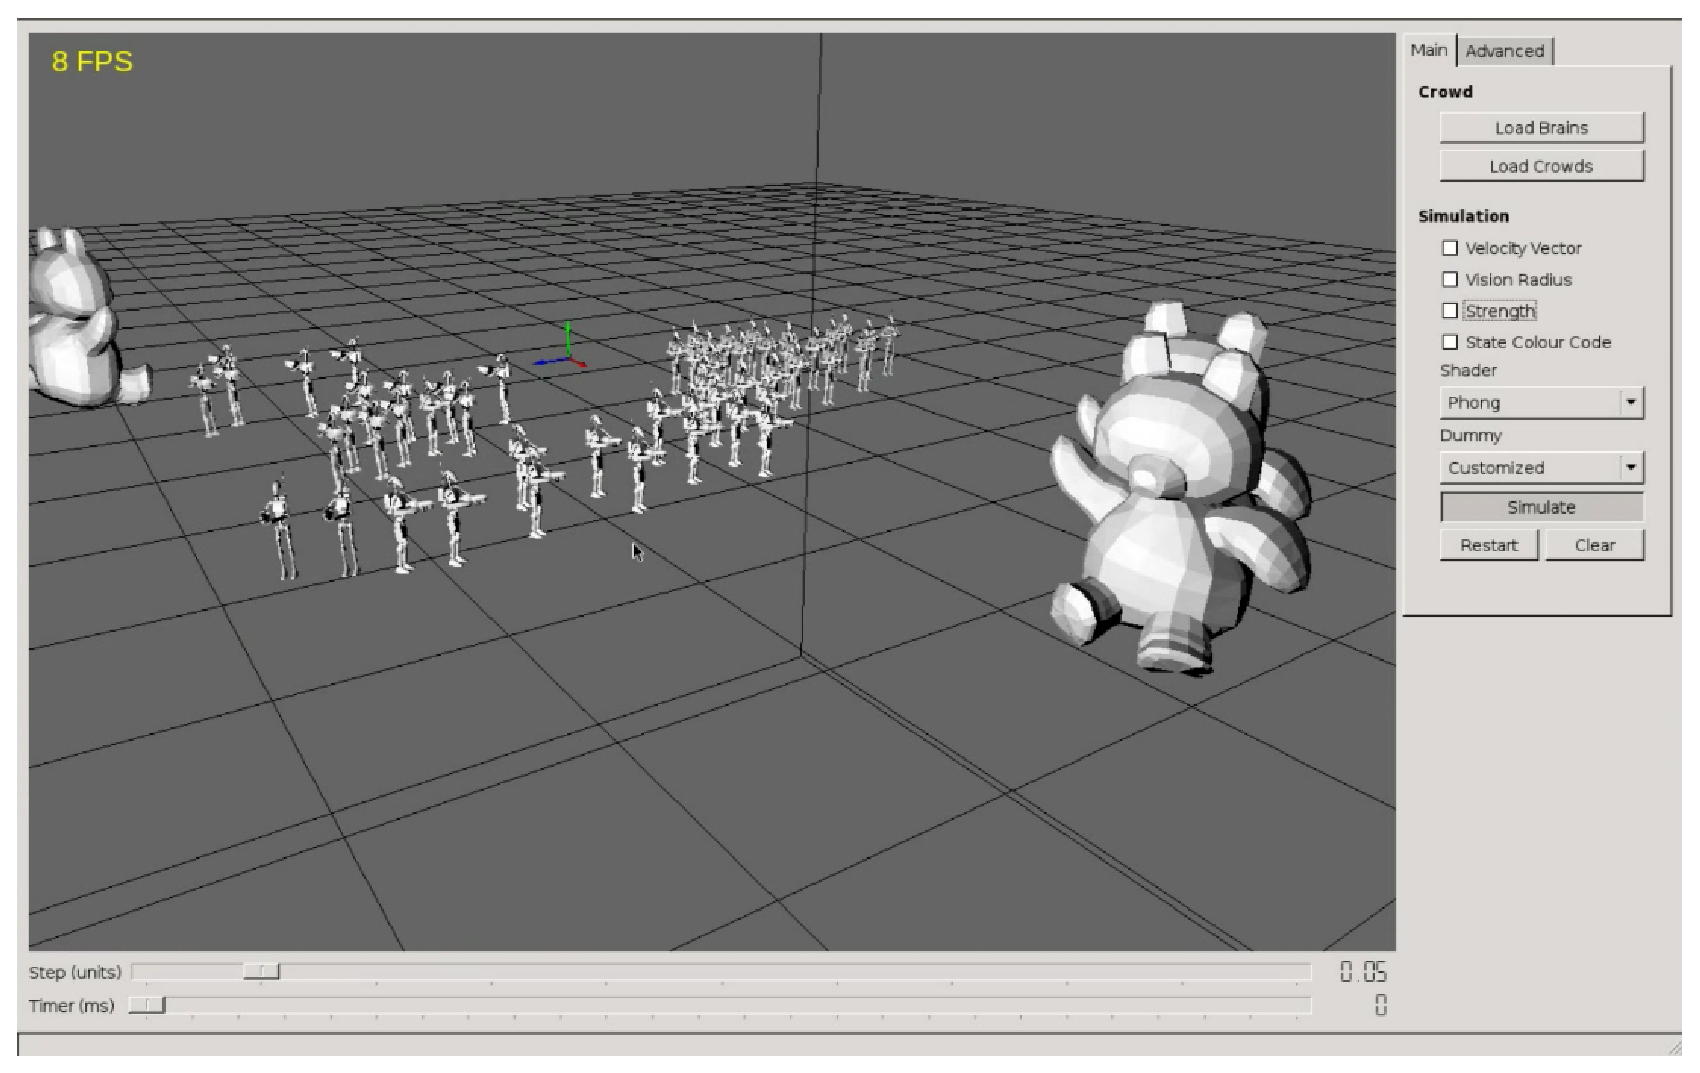
\includegraphics[scale=0.5]{droids_01.eps}
  \caption{Droids and targets}
\end{figure}

They patrol in flocks (green state), so that means that the three Reynolds' flocking algorithm rules are present here too (and in most behaviours). On the simulation there also are some targets which move randomly on the ground. When a droid sights a target (it enters in its vision radius), it changes of state and start attacking (res state). Targets receive the shots as messages and they decrease their strength. If a target gets too close to a droid, this permutes to a state of evasion to reach a proper distance to shot again (blue state). The FSM is presented below.

\begin{figure}[!h]
  \centering
 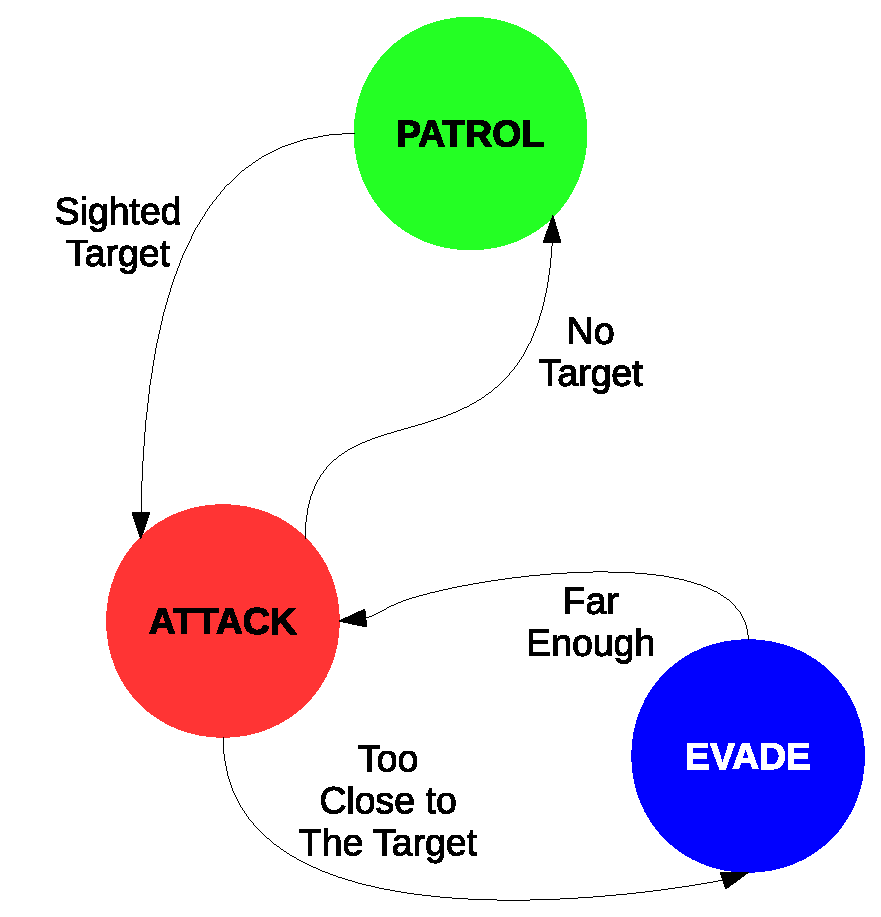
\includegraphics[scale=0.35]{droidFSM.eps}
  \caption{Droid's FSM}
\end{figure}

In the next screen captures it can be observed the group behaviour that arises. They stay at certain distance and attack together, tending to describe arcs around the target. Even if the attack state does not implement the flocking behaviour they group due to common targets.

\begin{figure}[!h]
  \centering
  \begin{tabular}{c c}
  	\subfloat[Droids flocks attacking targets]{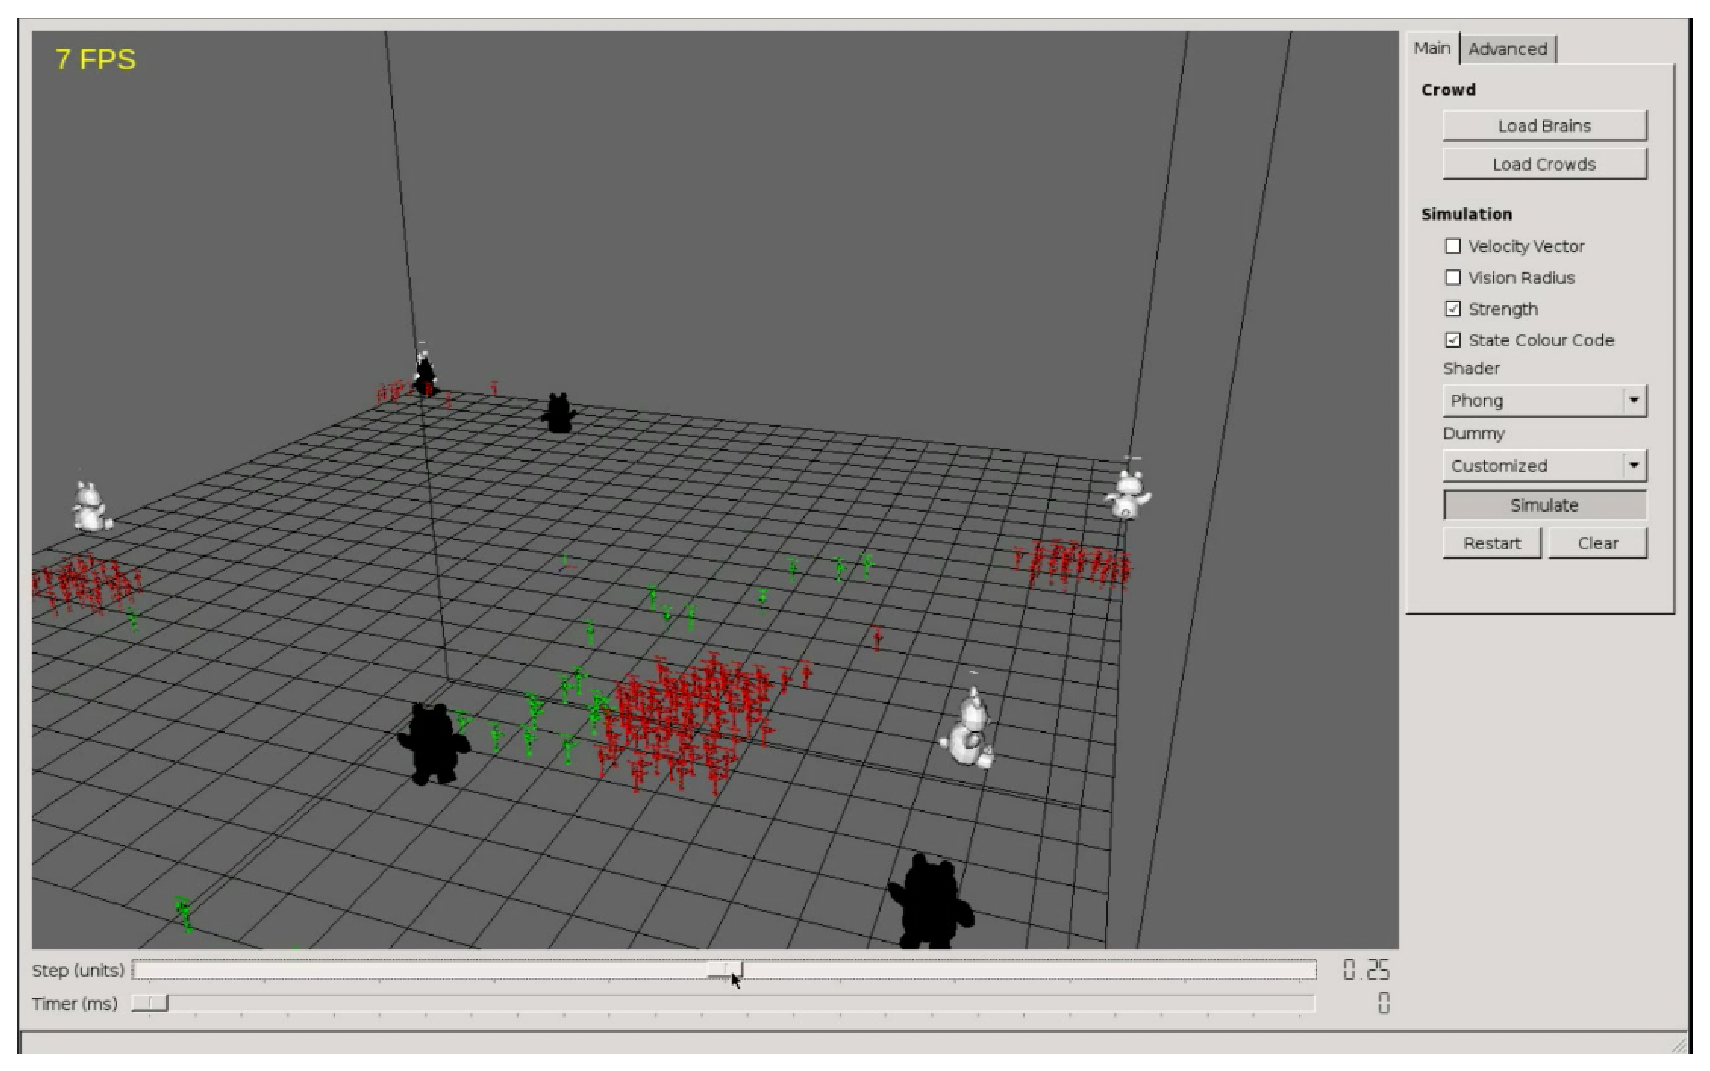
\includegraphics[scale=0.24]{droids_02.eps}} &
 	\subfloat[Droids evading]{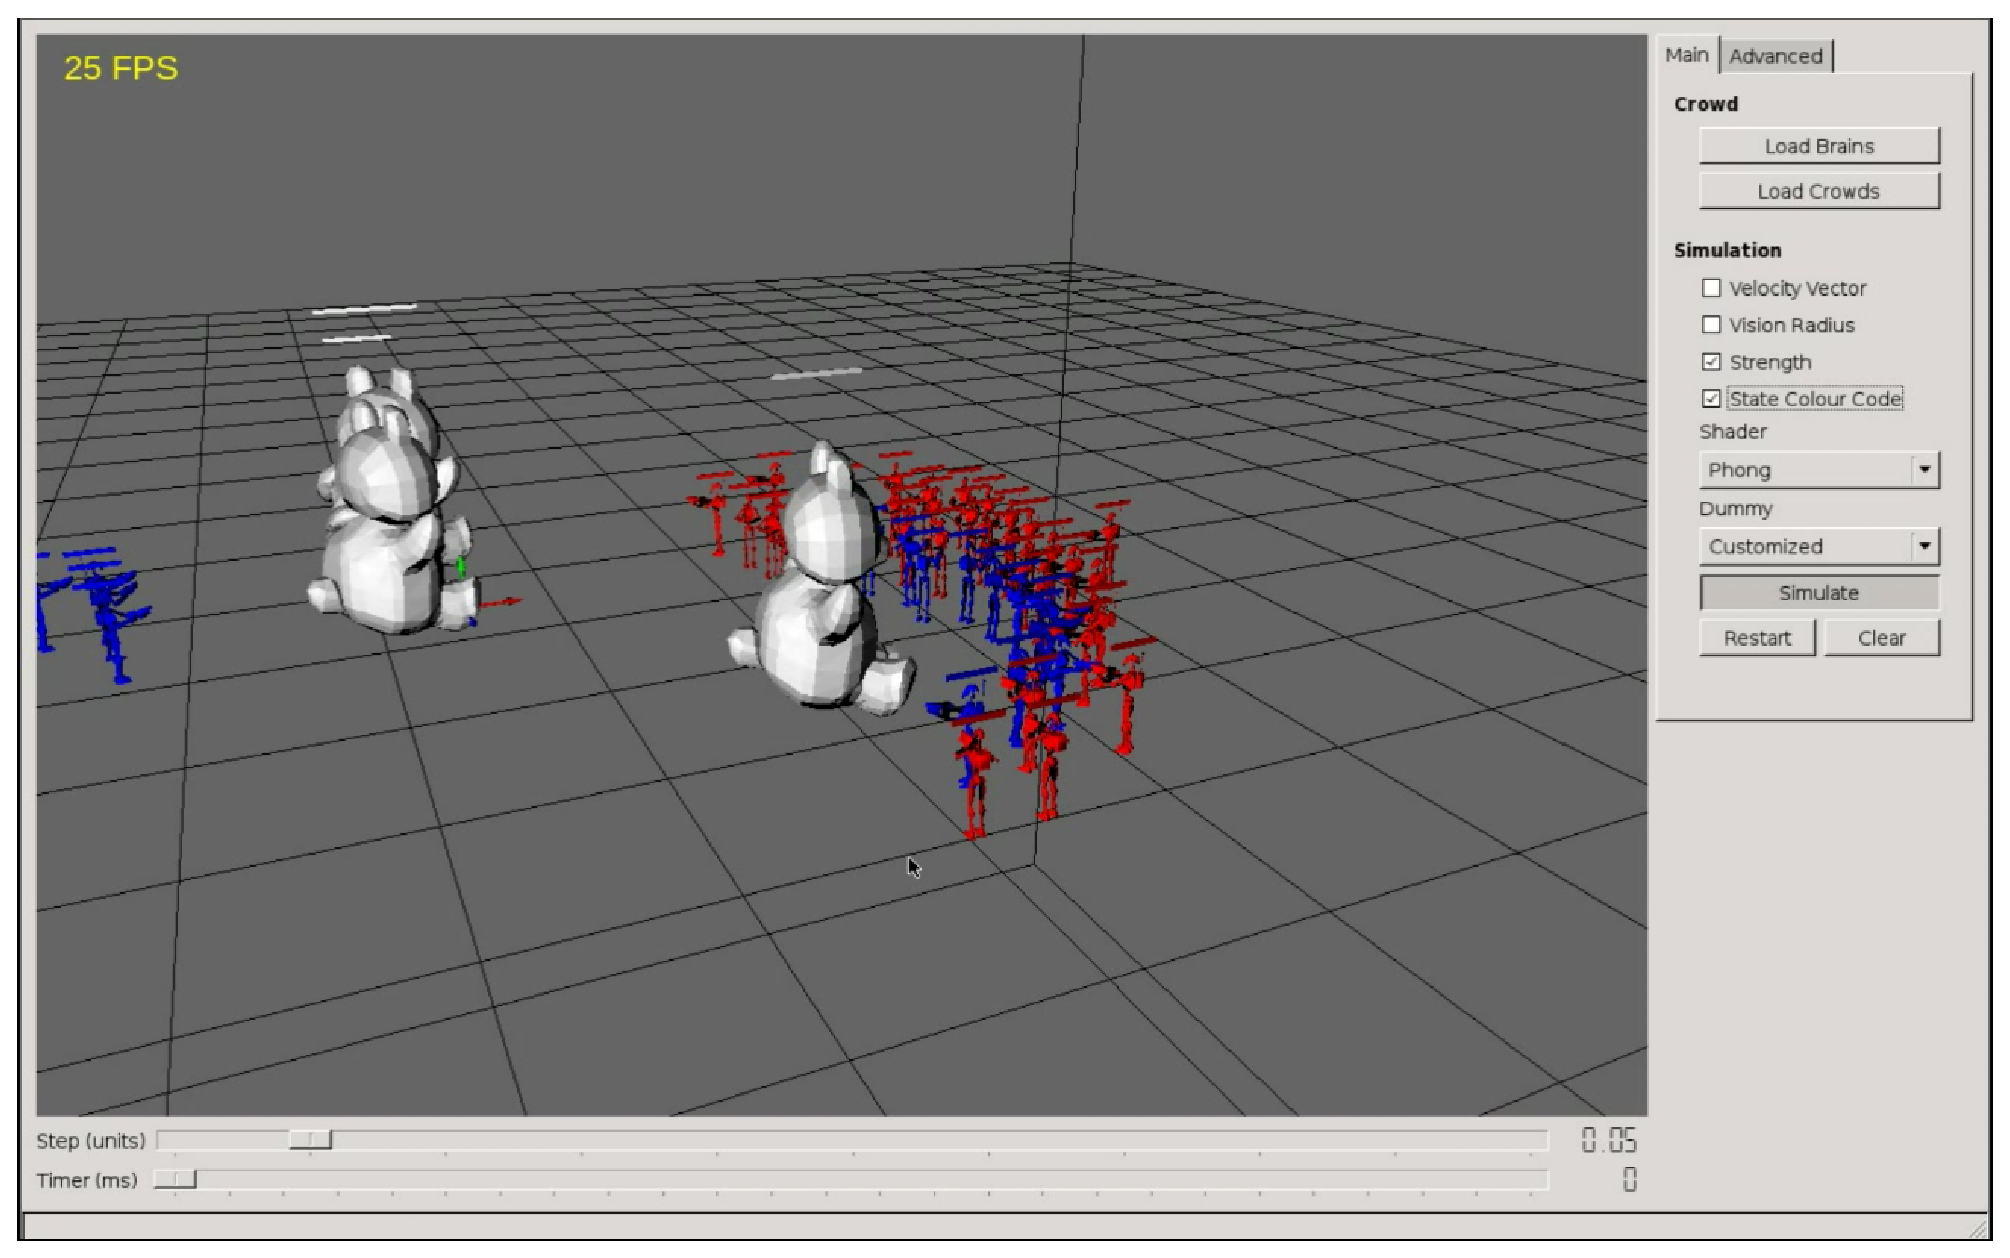
\includegraphics[scale=0.2]{droids_03.eps}} \\
 \end{tabular}
  \caption{Droids War Simulation}
\end{figure}

\subsection{Zombie Apocalypse}

This brain is the less complex one. This is quite logical if we take into account that we are trying to represent zombies. It is just an obsessive behaviour which launchs the agent against the \emph{wall}, trying to reach a target point by any mean.  

\begin{figure}[!h]
  \centering
  \begin{tabular}{c c}
  	\subfloat[Obsessive zombies running to the wall]{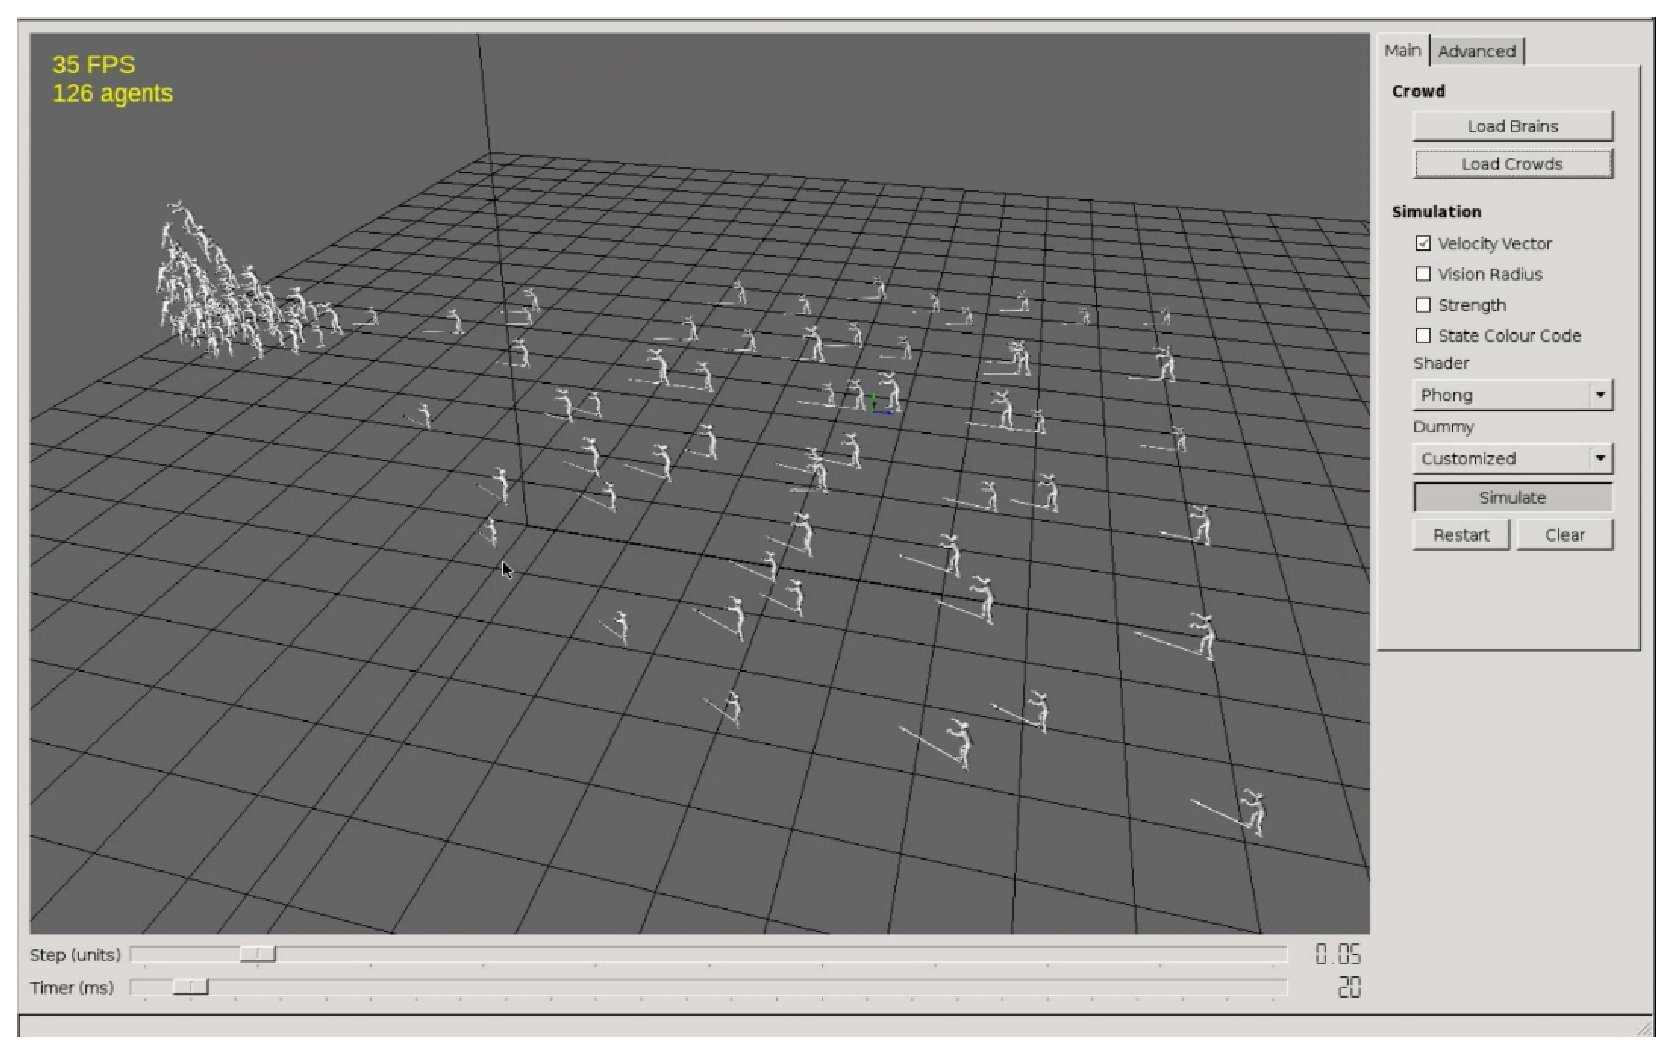
\includegraphics[scale=0.25]{zombies_01.eps}} &
 	\subfloat[Zombies climbing to the wall]{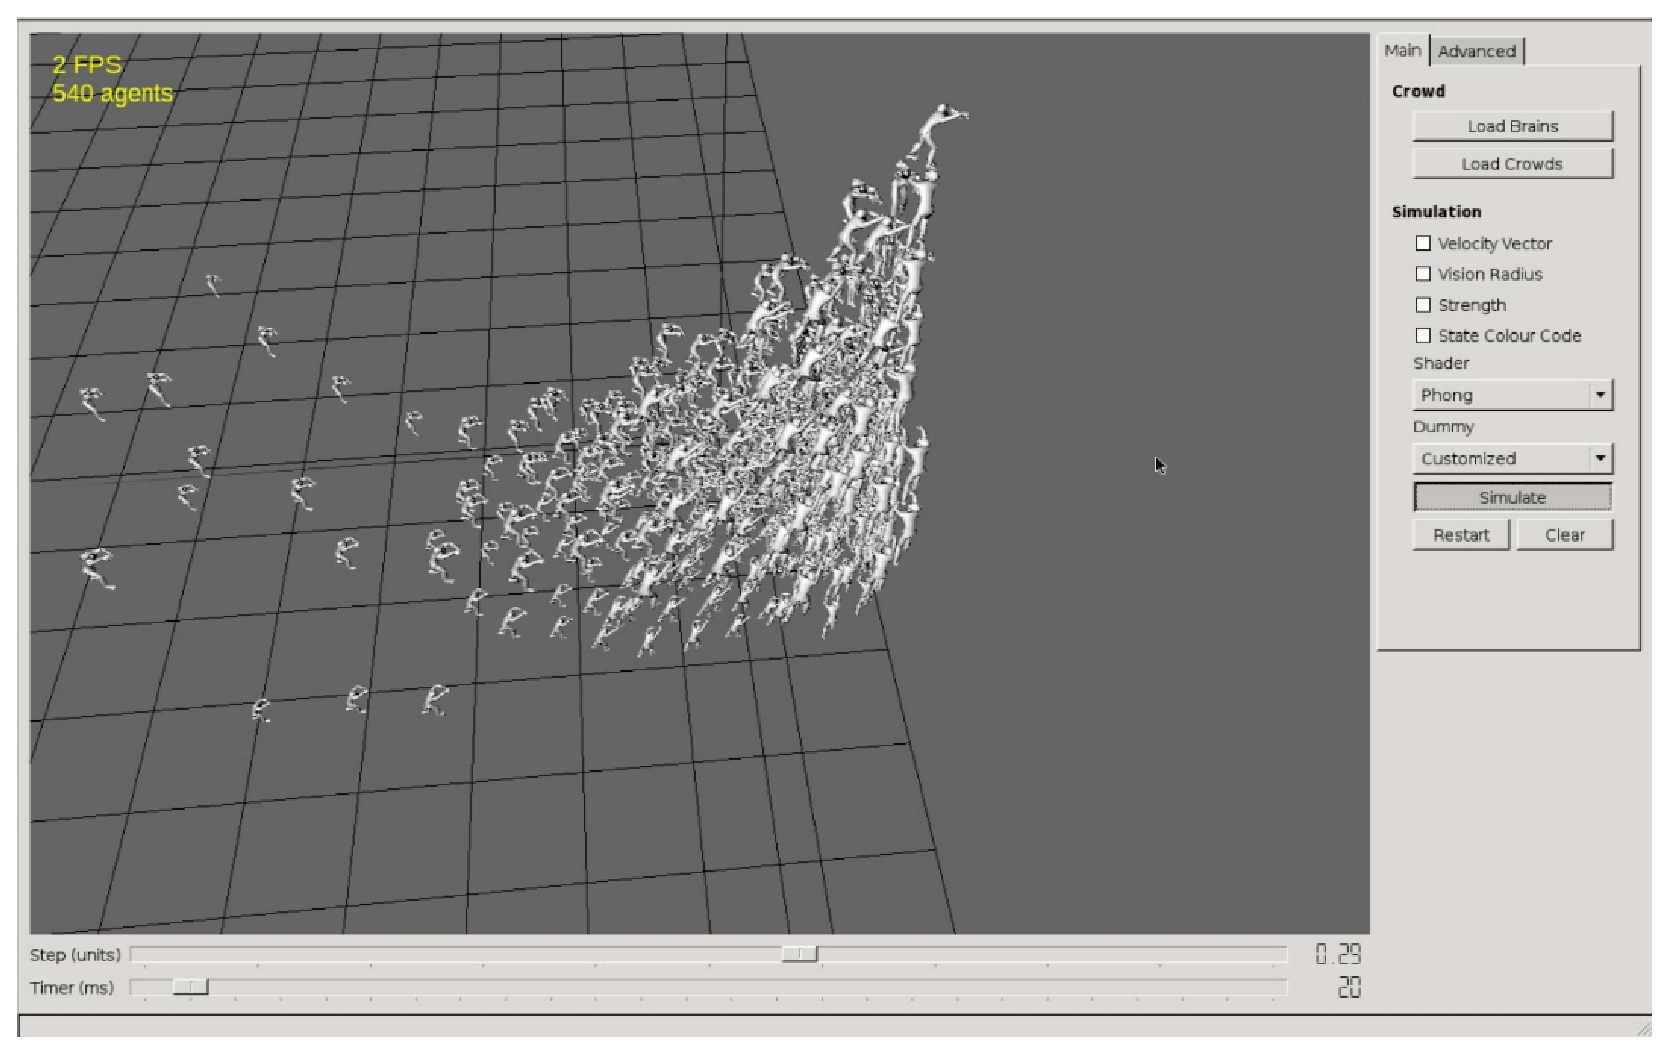
\includegraphics[scale=0.25]{zombies_02.eps}} \\
 \end{tabular}
  \caption{Zombie Apocalypse Simulation}
  \label{fig:zombieCaptures}
\end{figure}

What does the work in here is the sphere-based physics engine, which  projects the velocity over the tangent to spheres on the colliding point. This allows that bigger agents climb on other smaller. With a simulation with number of agents large enough, the behaviour that emerges corresponds to a group of not too smart agents, climbing on one another to desperately reach their target, creating a huge human mountain.

\begin{figure}[!h]
  \centering
	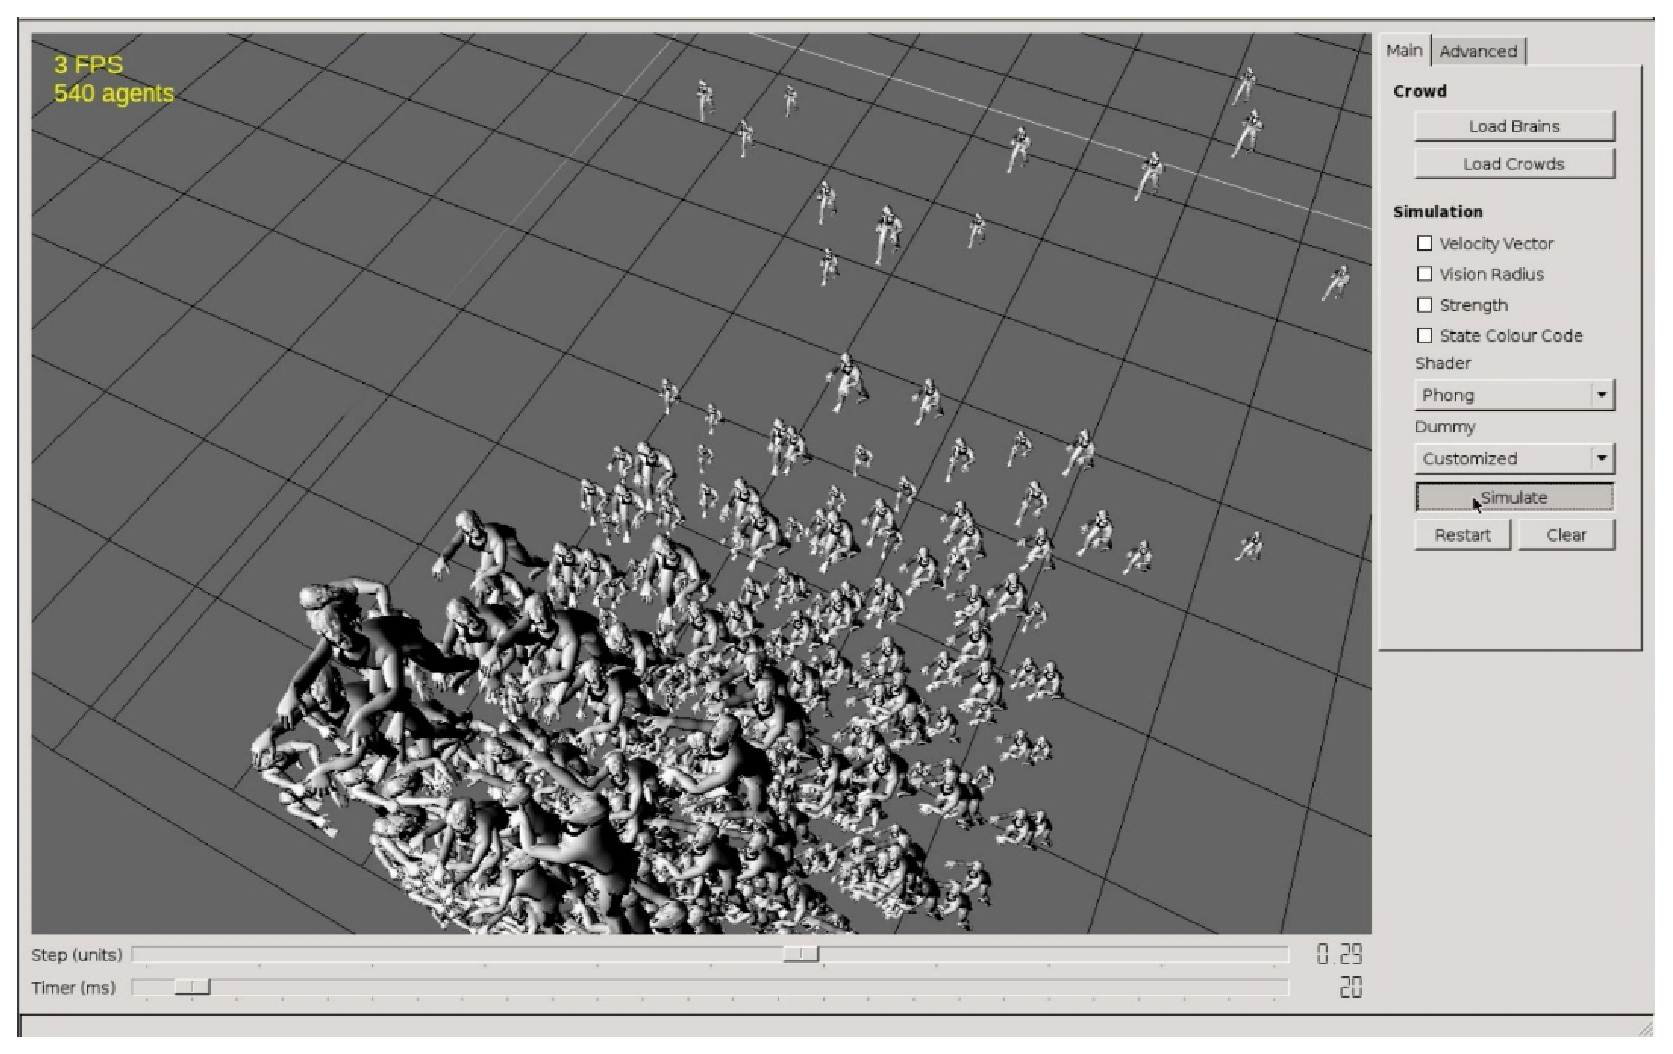
\includegraphics[scale=0.5]{zombies_03.eps}
	\caption{Mountain of zombies}
  \label{fig:zombieCaptures}
\end{figure}

\newpage
\subsection{A Battlefield}

This example might be the more complete one, it includes several behaviours with different characteristics that, by means of message passing, can communicate among all of them. The \emph{warrior} brain, is the classical member of a battle. It moves with their troop and when it sights an enemy it attacks it. Contrary to the shooter behaviour, this is a body-to-body fight so a warrior can send attacks to the enemy stepping forward, or recieve attacks having step back. If the strength is too critical, the warrior switch to state of defense, send not attack and recovering strength. The FSM is presented below.

\begin{figure}[!h]
  \centering
 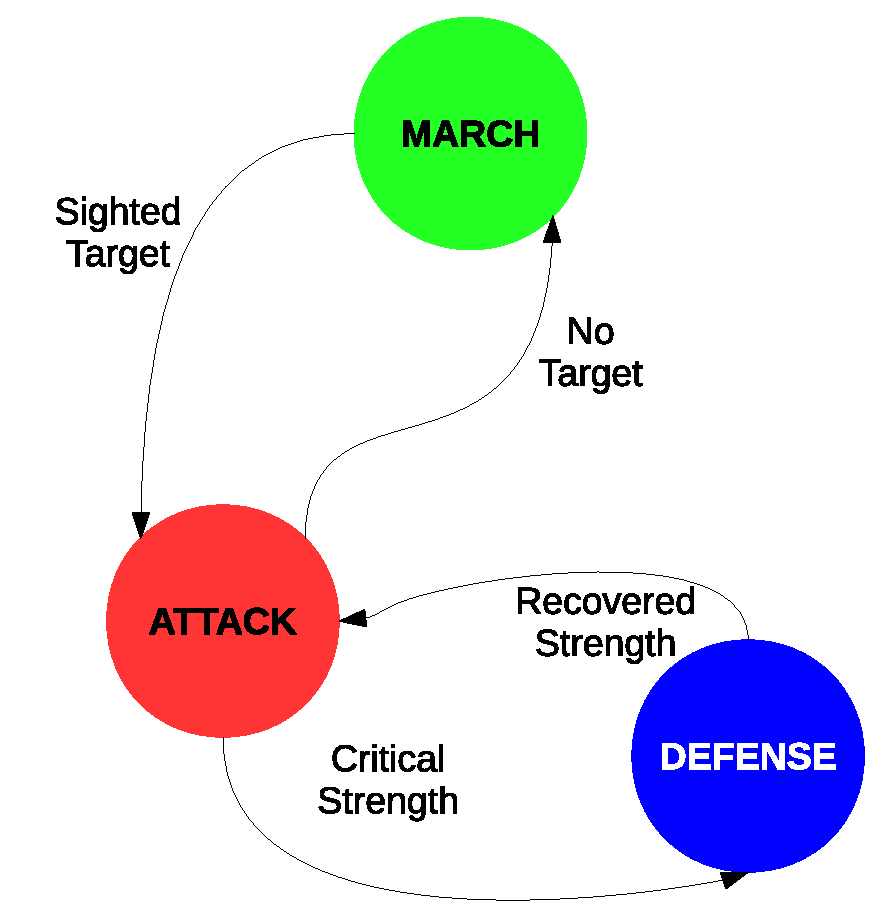
\includegraphics[scale=0.35]{warriorFSM.eps}
  \caption{Warrior's FSM}
\end{figure}

In the same, it was developed a very similar brain to the warrior called \emph{captain}. The captain commands warriors and has to lead troop to the enemy. Thus, he has extra movement freedom besides the flocking properties. It is similar to a leader boid.

The emergent behaviours that may arise in this situations are infinite. Normally after the clash of two armies, the warrior will start to join in small groups, such as couples or three or four, fighting among them. Warriors that do not sight the enemy will march together where, although the movement may be highly synchronous, their physical properties will condition their march.

\begin{figure}[!h]
  \centering
  \begin{tabular}{c c}
  	\subfloat[Fighting behaviours]{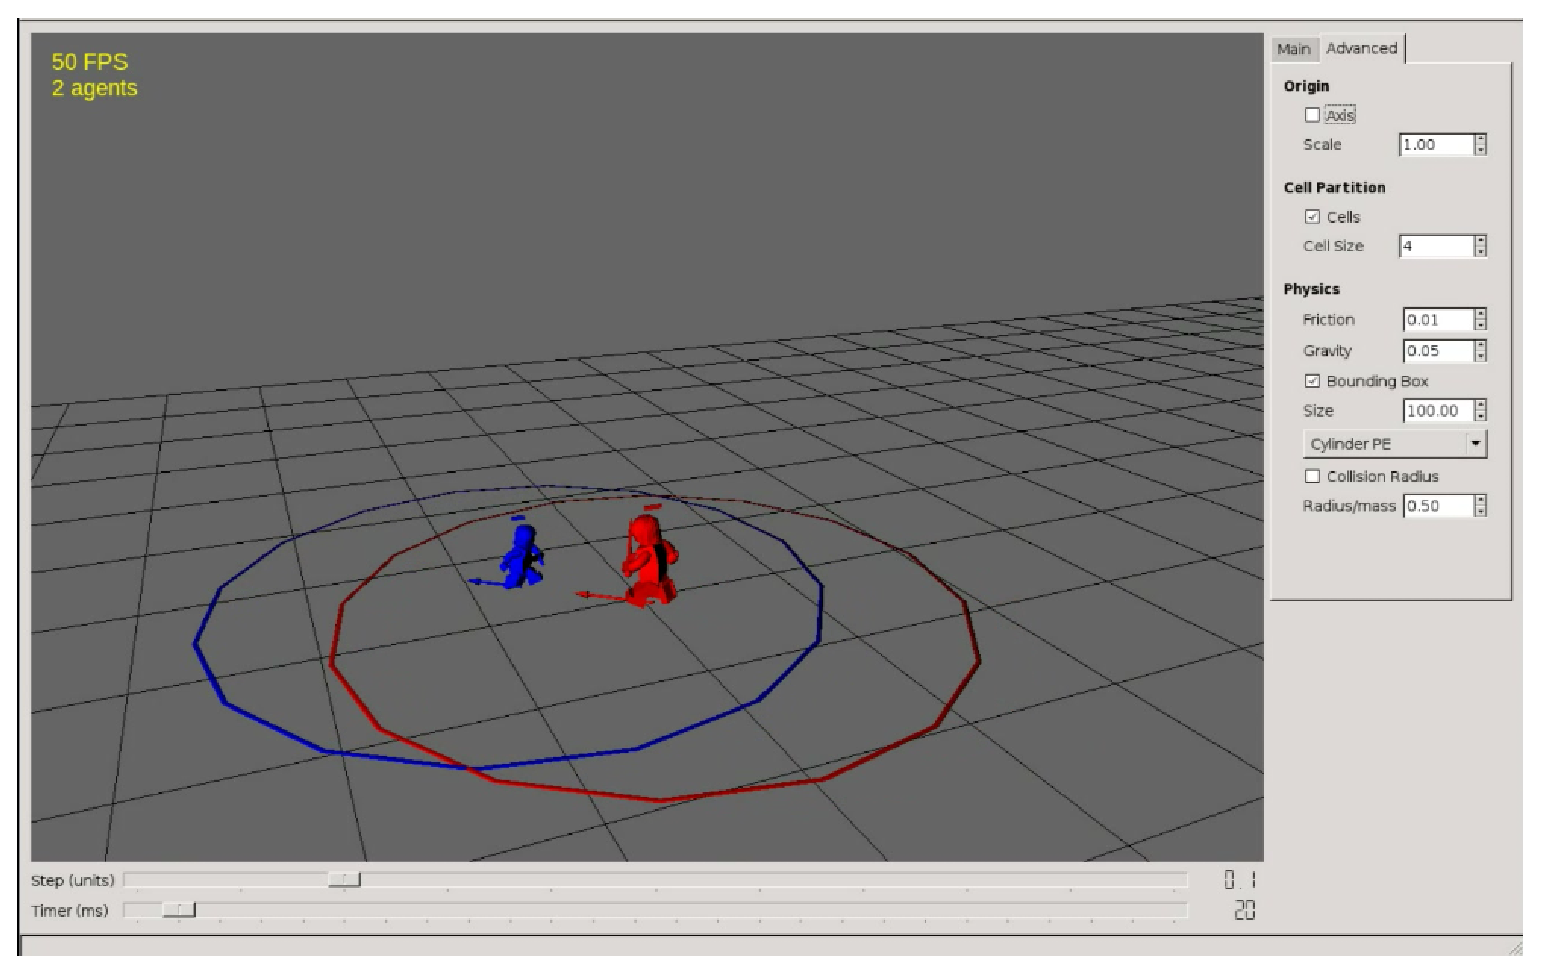
\includegraphics[scale=0.28]{battle_01.eps}} &
 	\subfloat[Sparse battlefield]{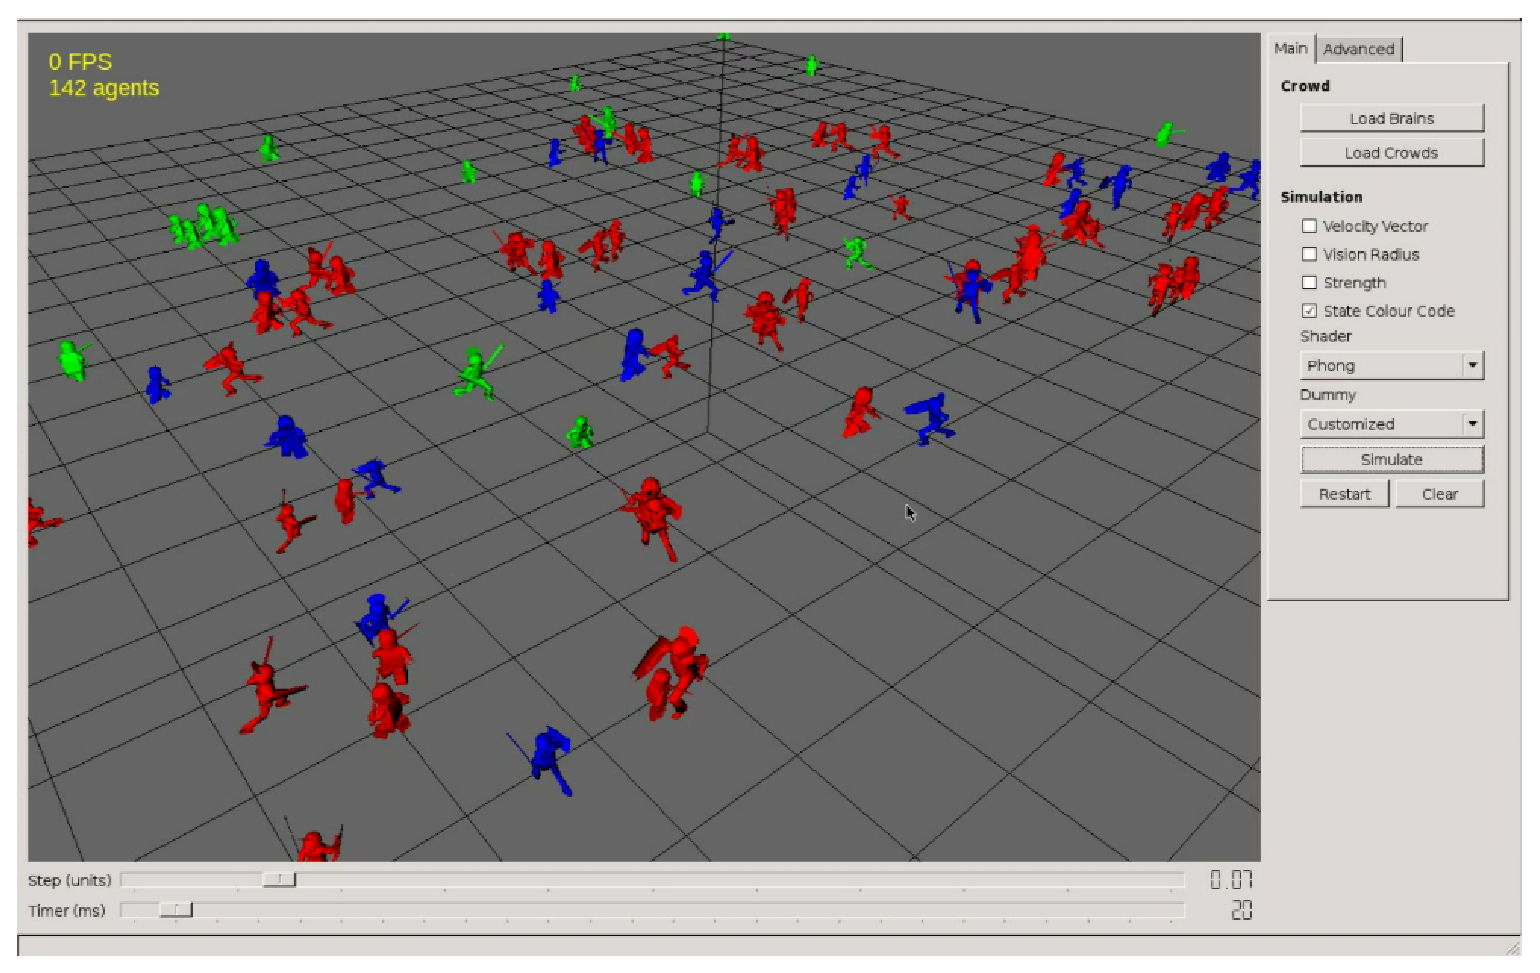
\includegraphics[scale=0.28]{battle_02.eps}} \\
 	\subfloat[Dense battlefield]{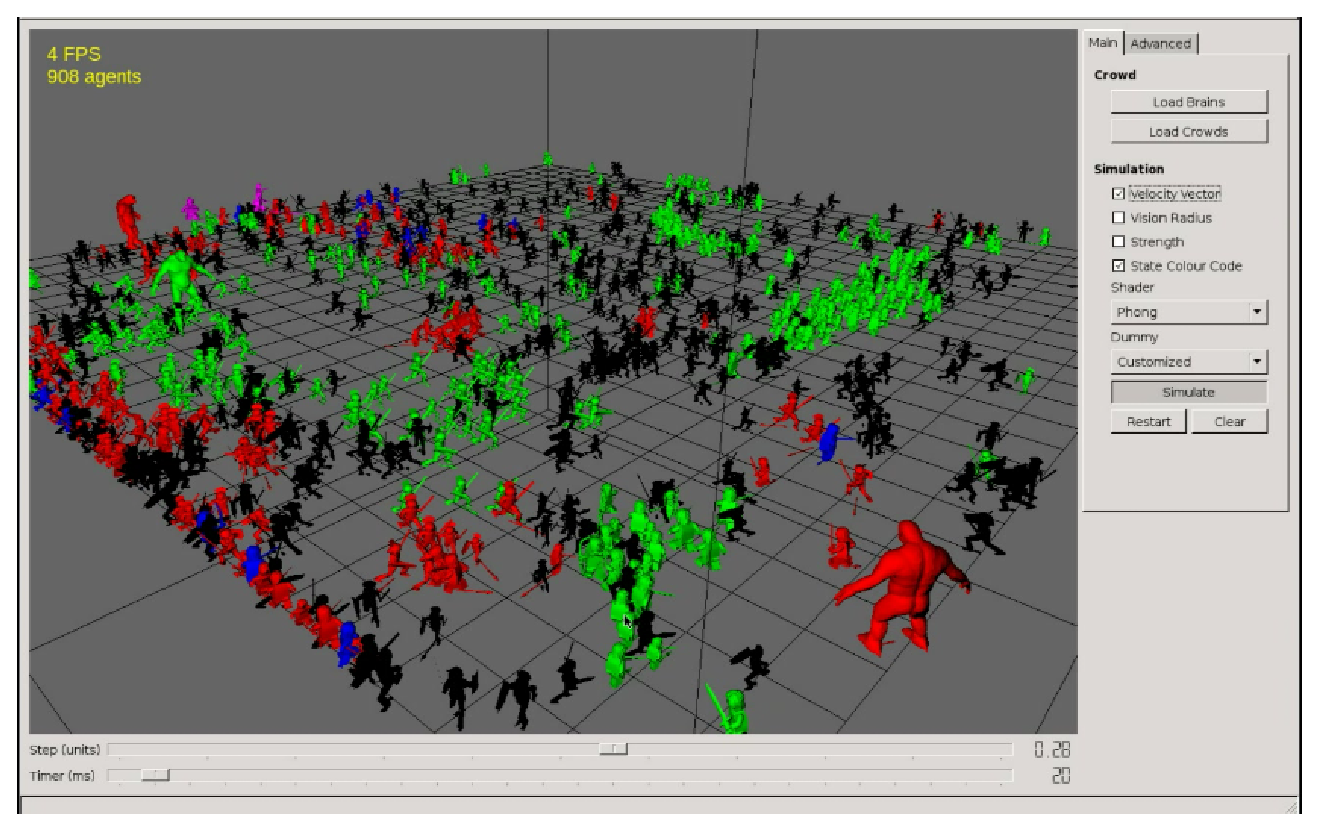
\includegraphics[scale=0.33]{battle_03.eps}} &
 	\subfloat[Marching troops]{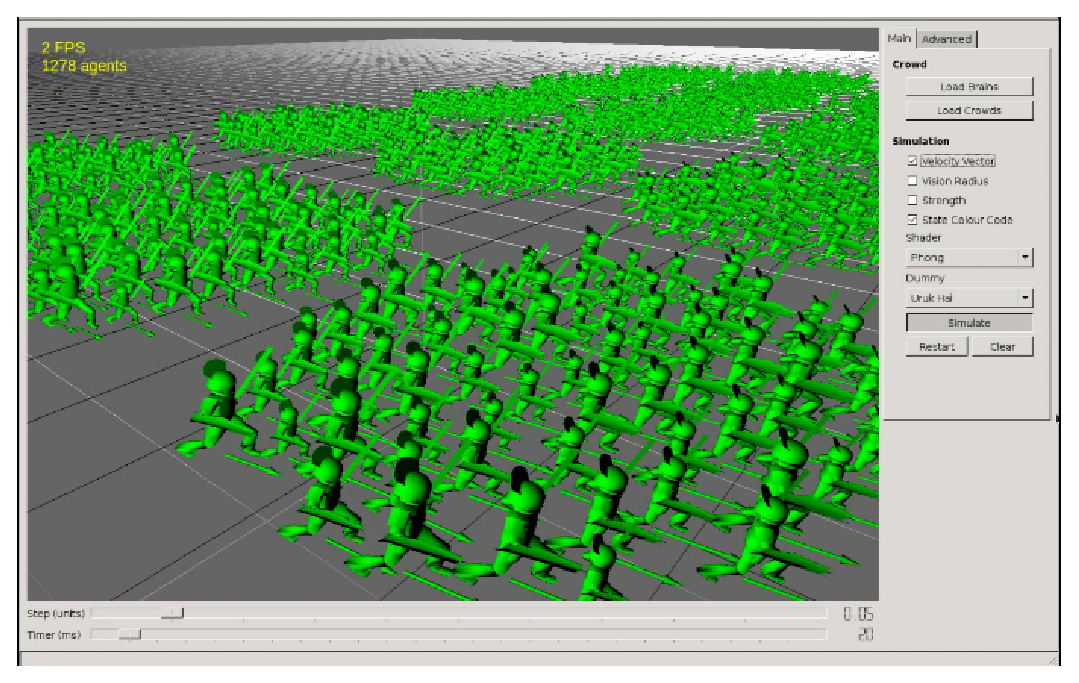
\includegraphics[scale=0.4]{battle_04.eps}} \\
 \end{tabular}
  \caption{A Battlefield Simulation}
  \label{fig:battleCaptures}
\end{figure}

In order to enrich the battlefield, some extra behaviours were also developed. The \emph{archer} brain is very similar to the shooter droid, and the \emph{troll}, although slower, is capable to apply attacks much stronger than a current warrior.

\begin{figure}[!h]
  \centering
  \begin{tabular}{c c}
  	\subfloat[Flock of archer behaviours]{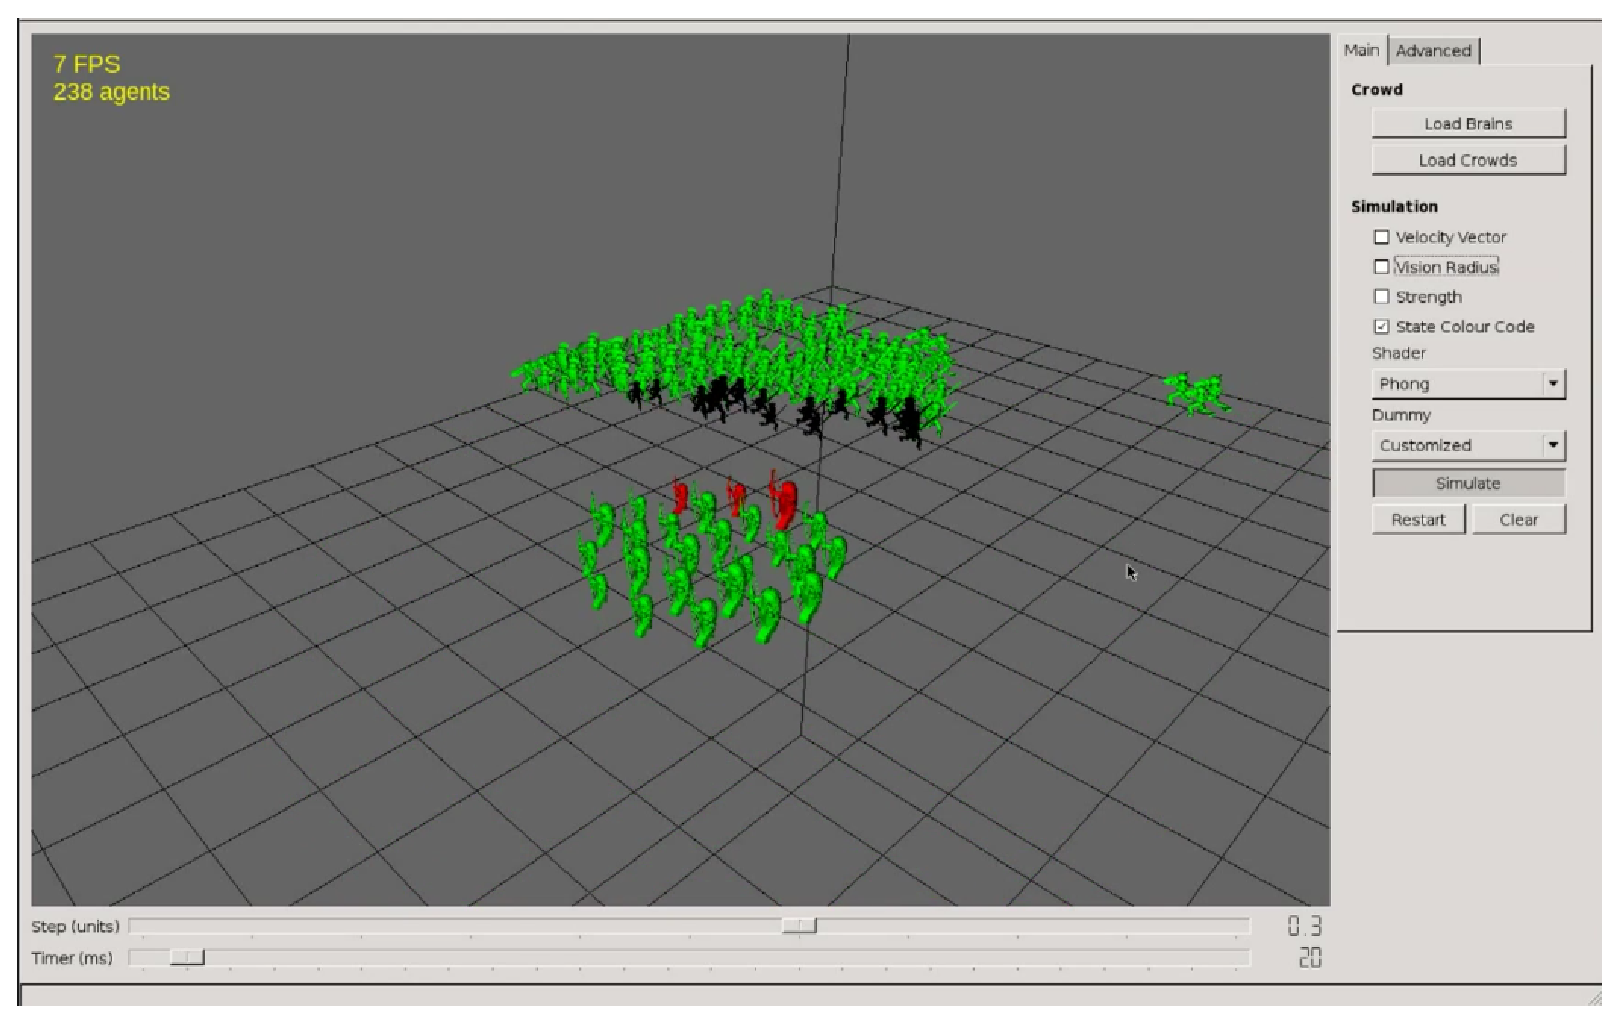
\includegraphics[scale=0.27]{archers.eps}} &
 	\subfloat[Troll behaviour]{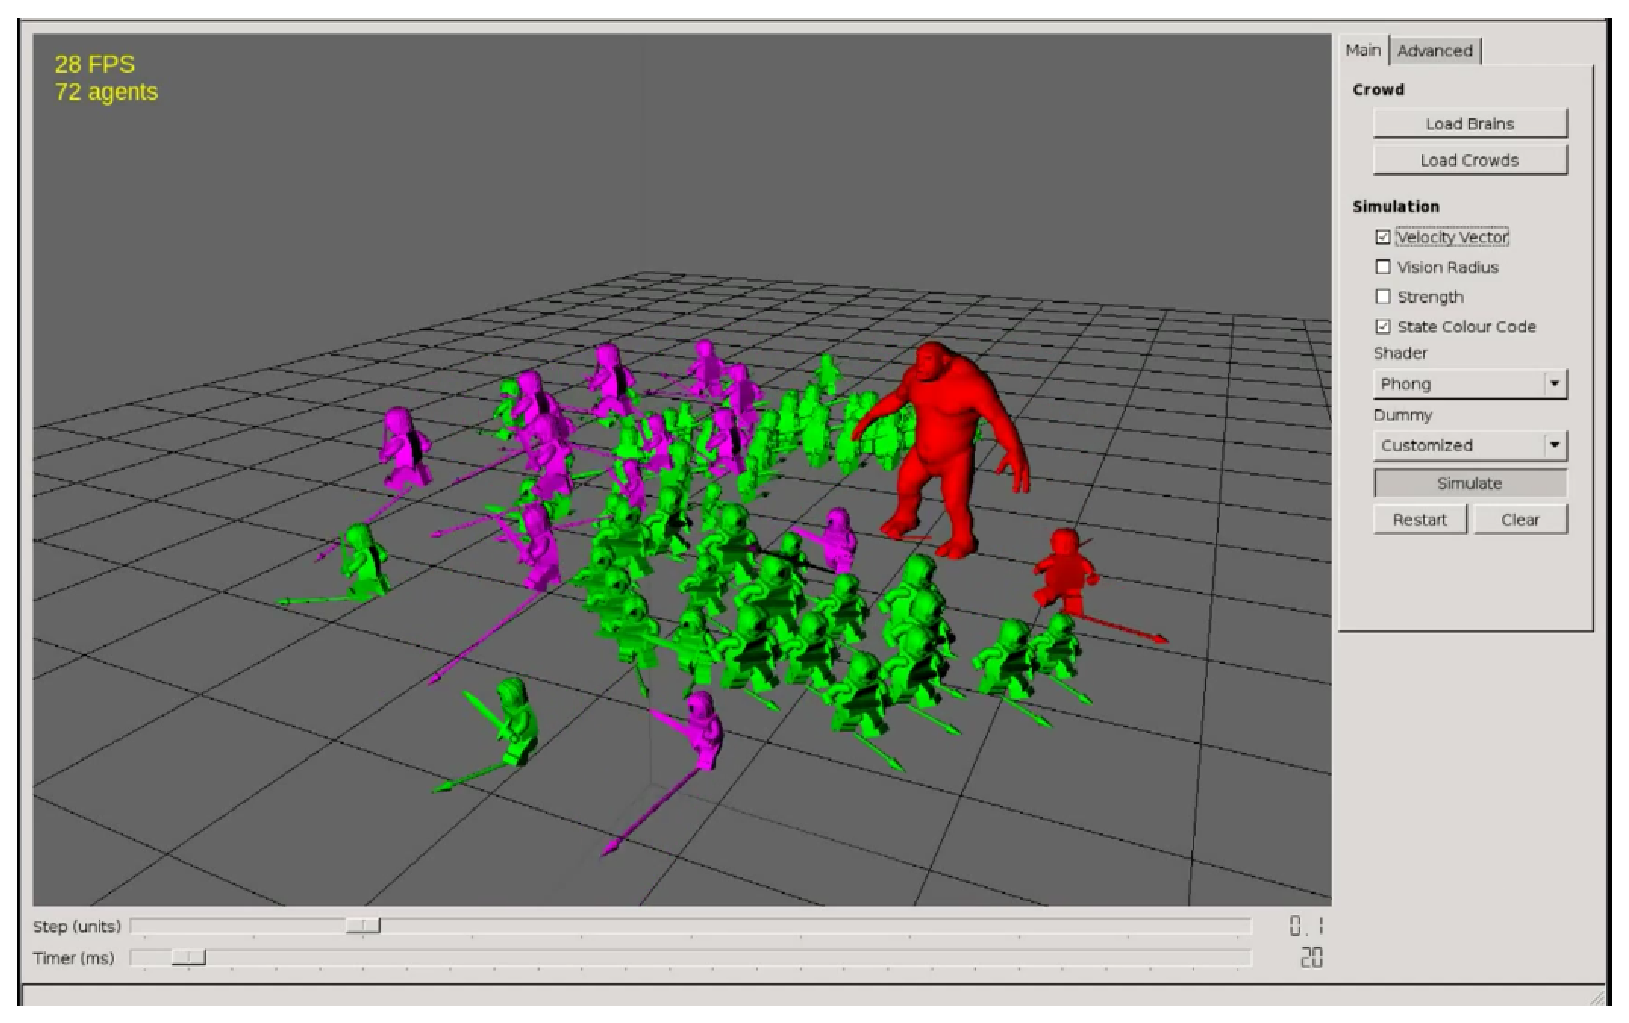
\includegraphics[scale=0.27]{troll.eps}} \\
 \end{tabular}
  \caption{Extra battle behaviours}
\end{figure}

\newpage
\subsection{A Ballroom}

To prove that not only war environments can be build with this approach, the next behaviour intends to represent A Ballroom. To achieve this, the mechanism was based in how an architecture of client-server works, , where the communication obtains an important role.

Firstly, we have the brain of a \emph{dancer}, which acts a passive dancer most of the time. She is waiting in the ballroom, moving randomly. The other brain is the \emph{danceLeader}, who will find for free dancers. The protocol works in this way: the danceLeader may say ``Shall we dance?'' and the dancer will accept the request.

\begin{figure}[!h]
  \centering
  \begin{tabular}{c c}
  	\subfloat[danceLeader FSM]{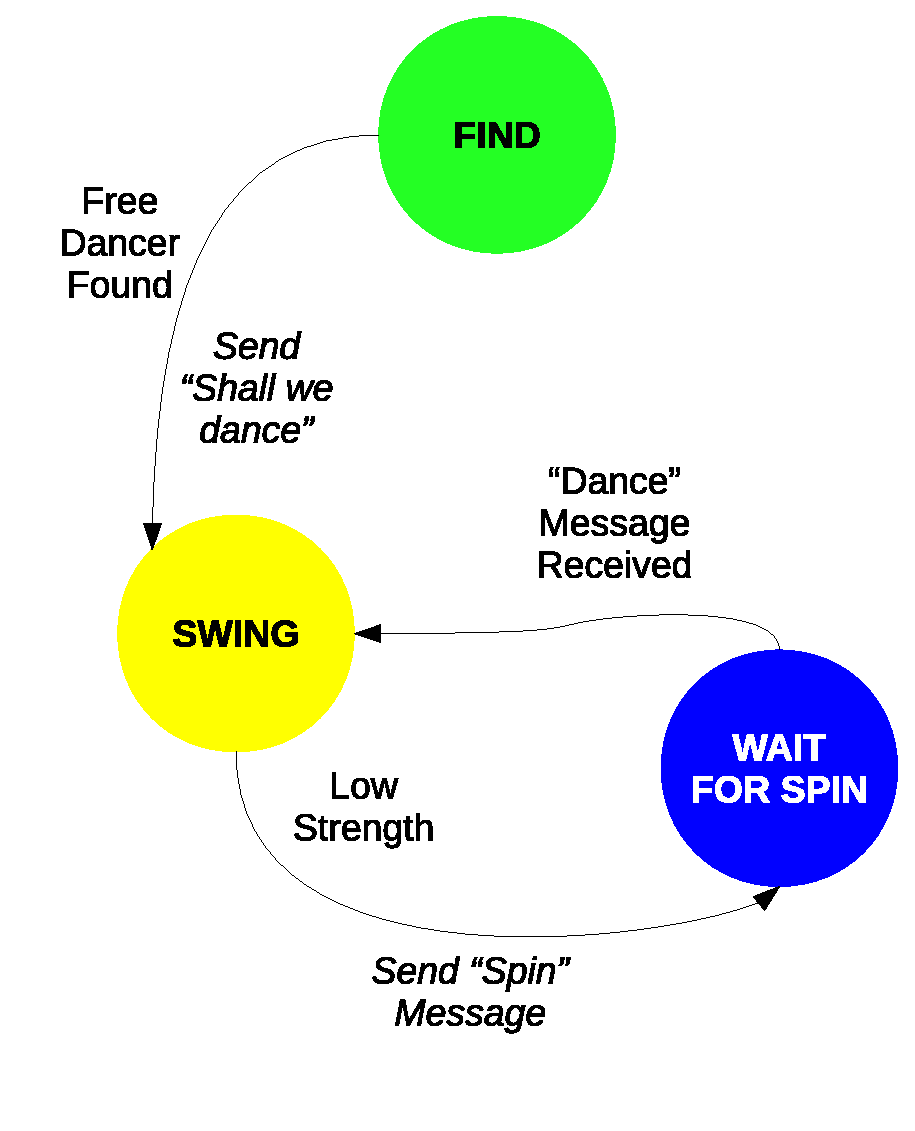
\includegraphics[scale=0.35]{danceLeaderFSM.eps}} &
 	\subfloat[dancer FSM]{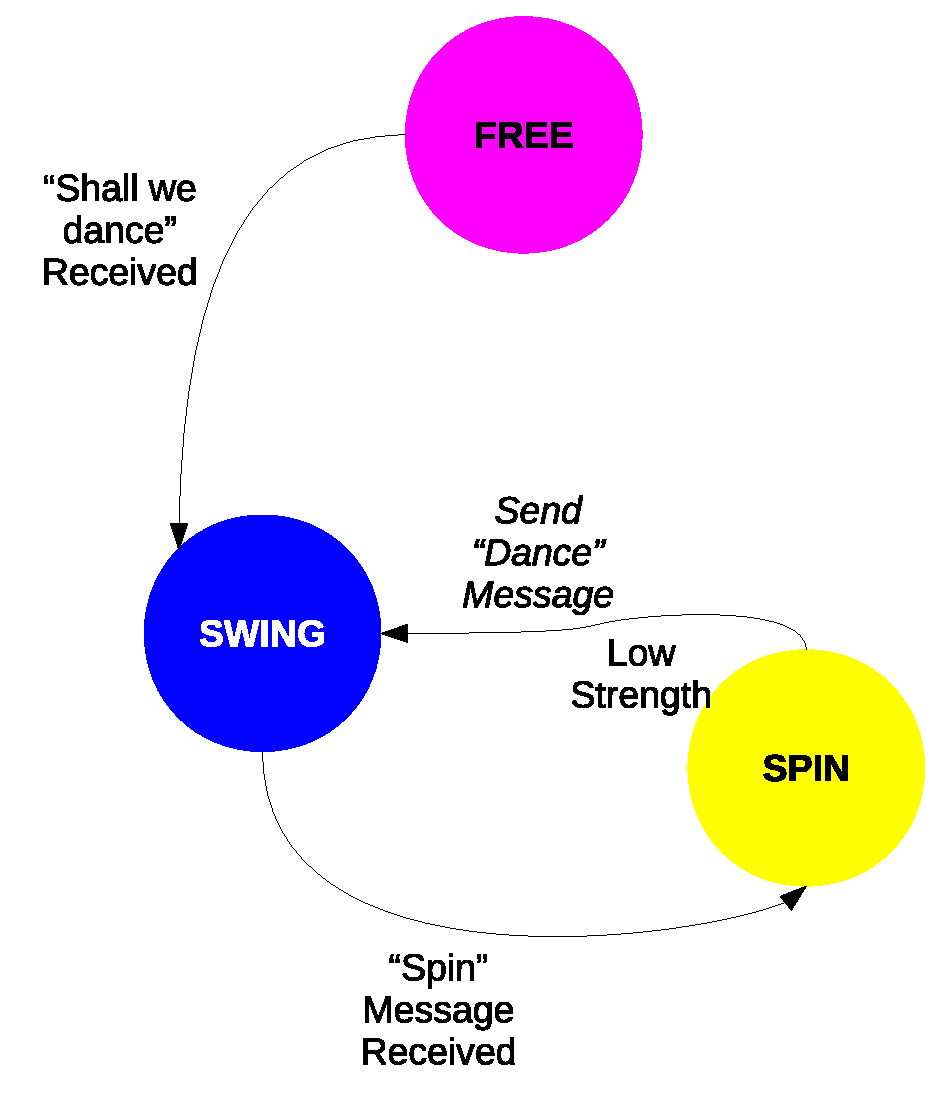
\includegraphics[scale=0.35]{dancerFSM.eps}} \\
 \end{tabular}
  \caption{FSM's for A Ballroom Simulation}
\end{figure}


The individual behaviour here may have two stages. First, danceLeaders try to find free dancers around the room and, once they find one, a couple dancing starts. Thus, the emergent group behaviour that can be observed here is very interesting; there will be many couples dancing and swinging graciously meanwhile some others are still finding or waiting to be found.

\begin{figure}[!h]
  \centering
  \begin{tabular}{c c}
  	\subfloat[Dancers finding partner]{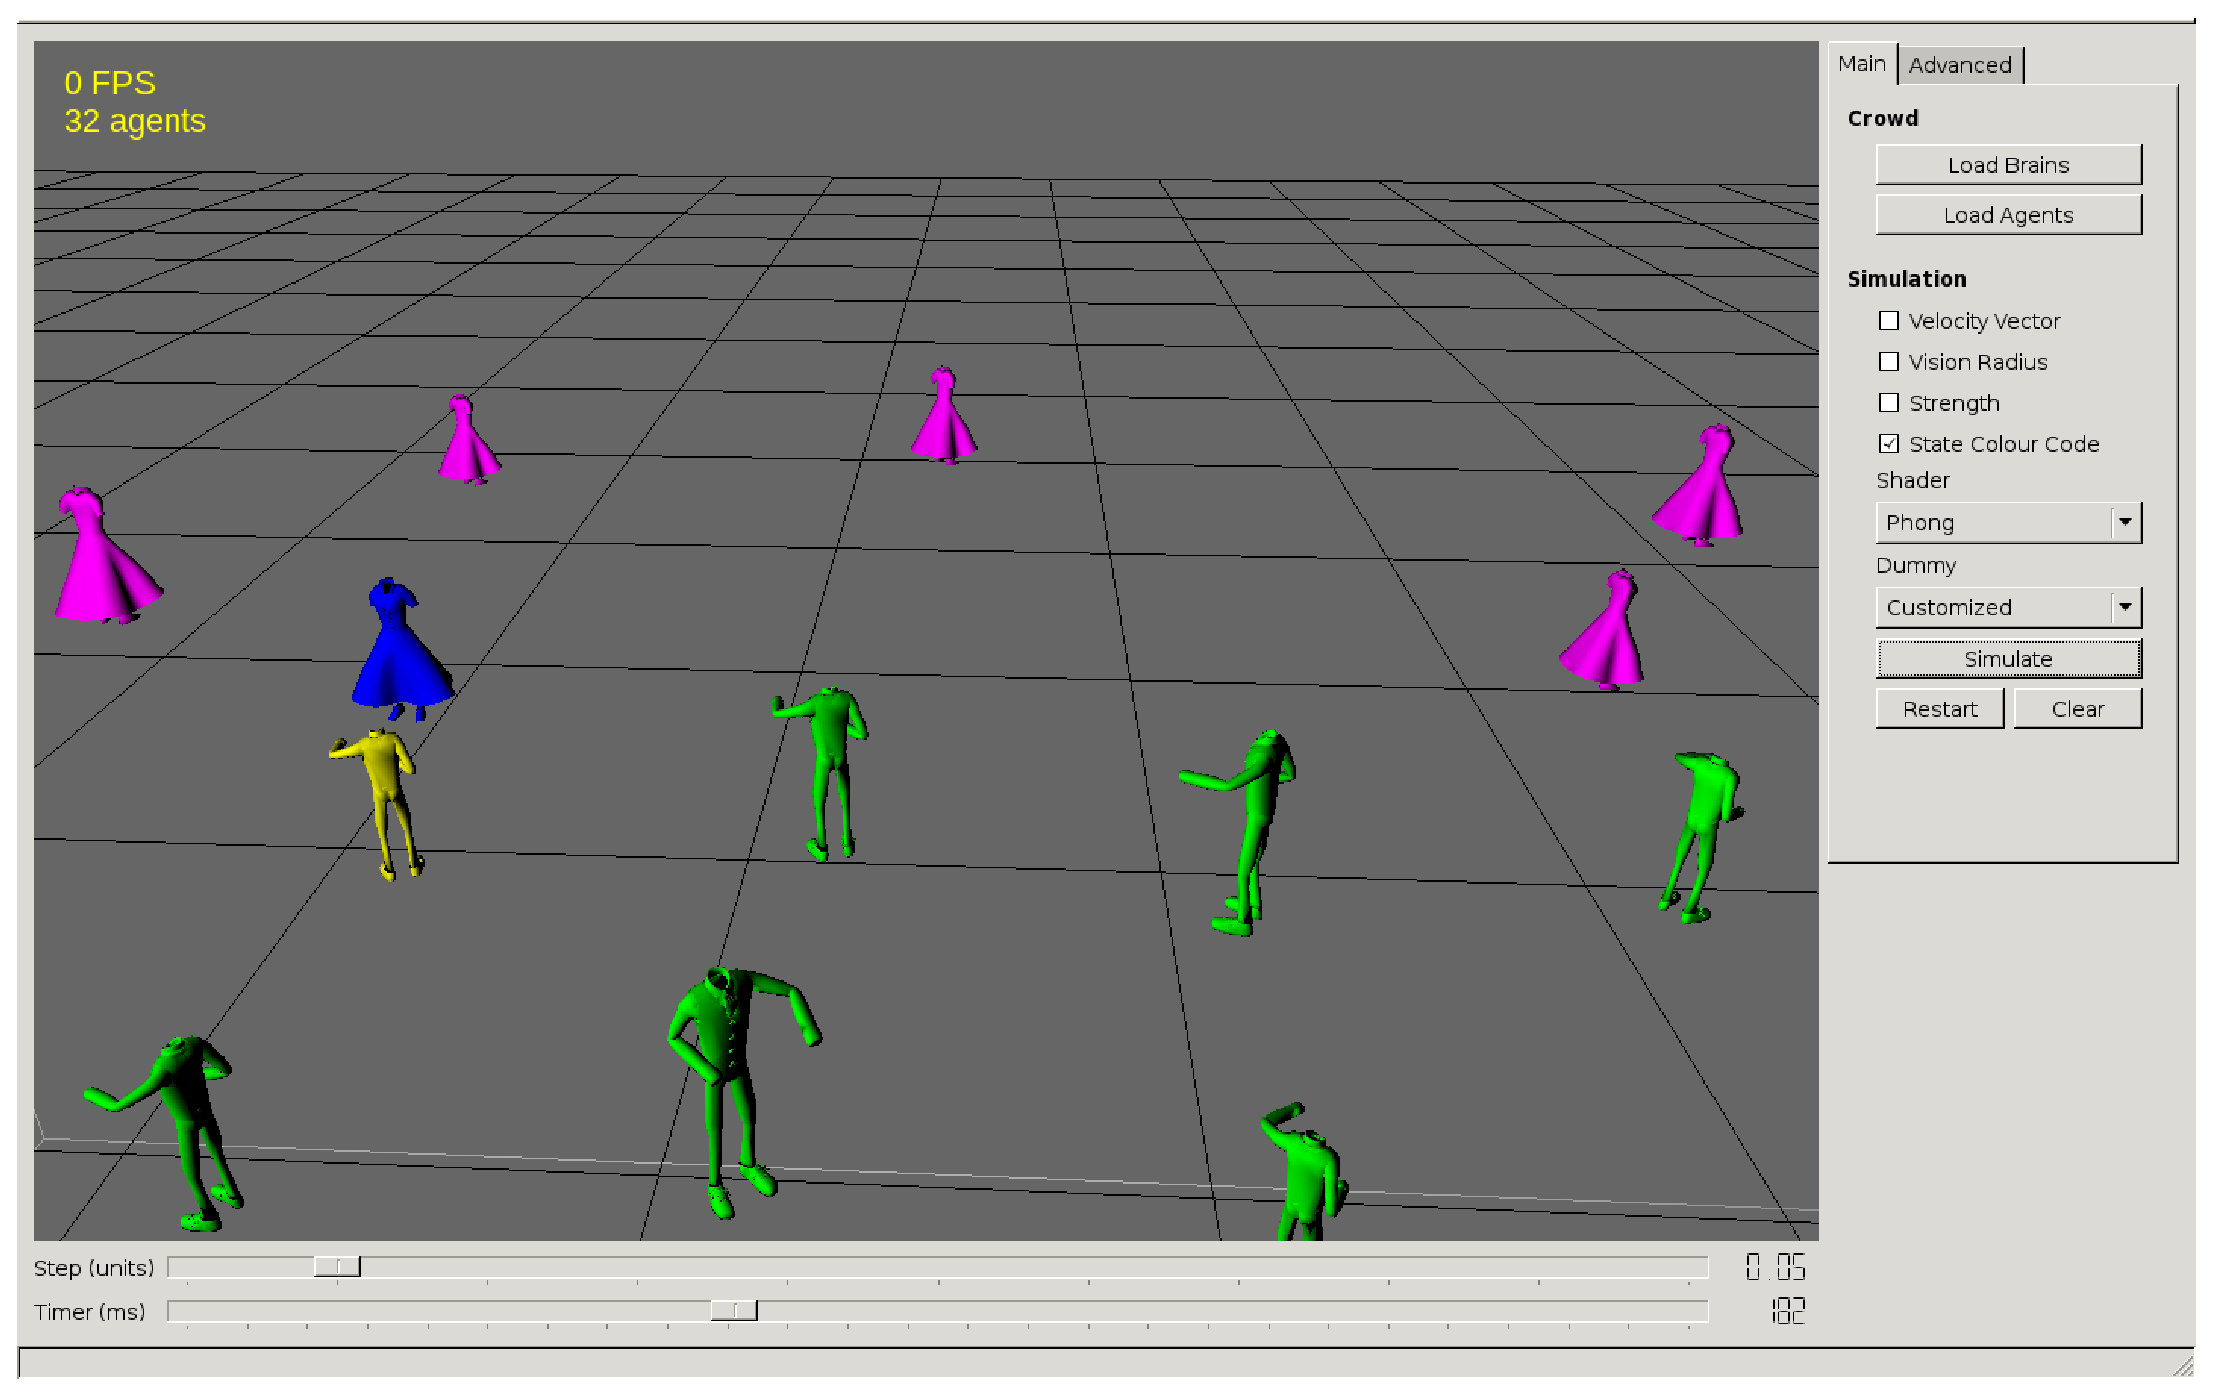
\includegraphics[scale=0.195]{ballroom_01.eps}} &
 	\subfloat[Couples swinging together]{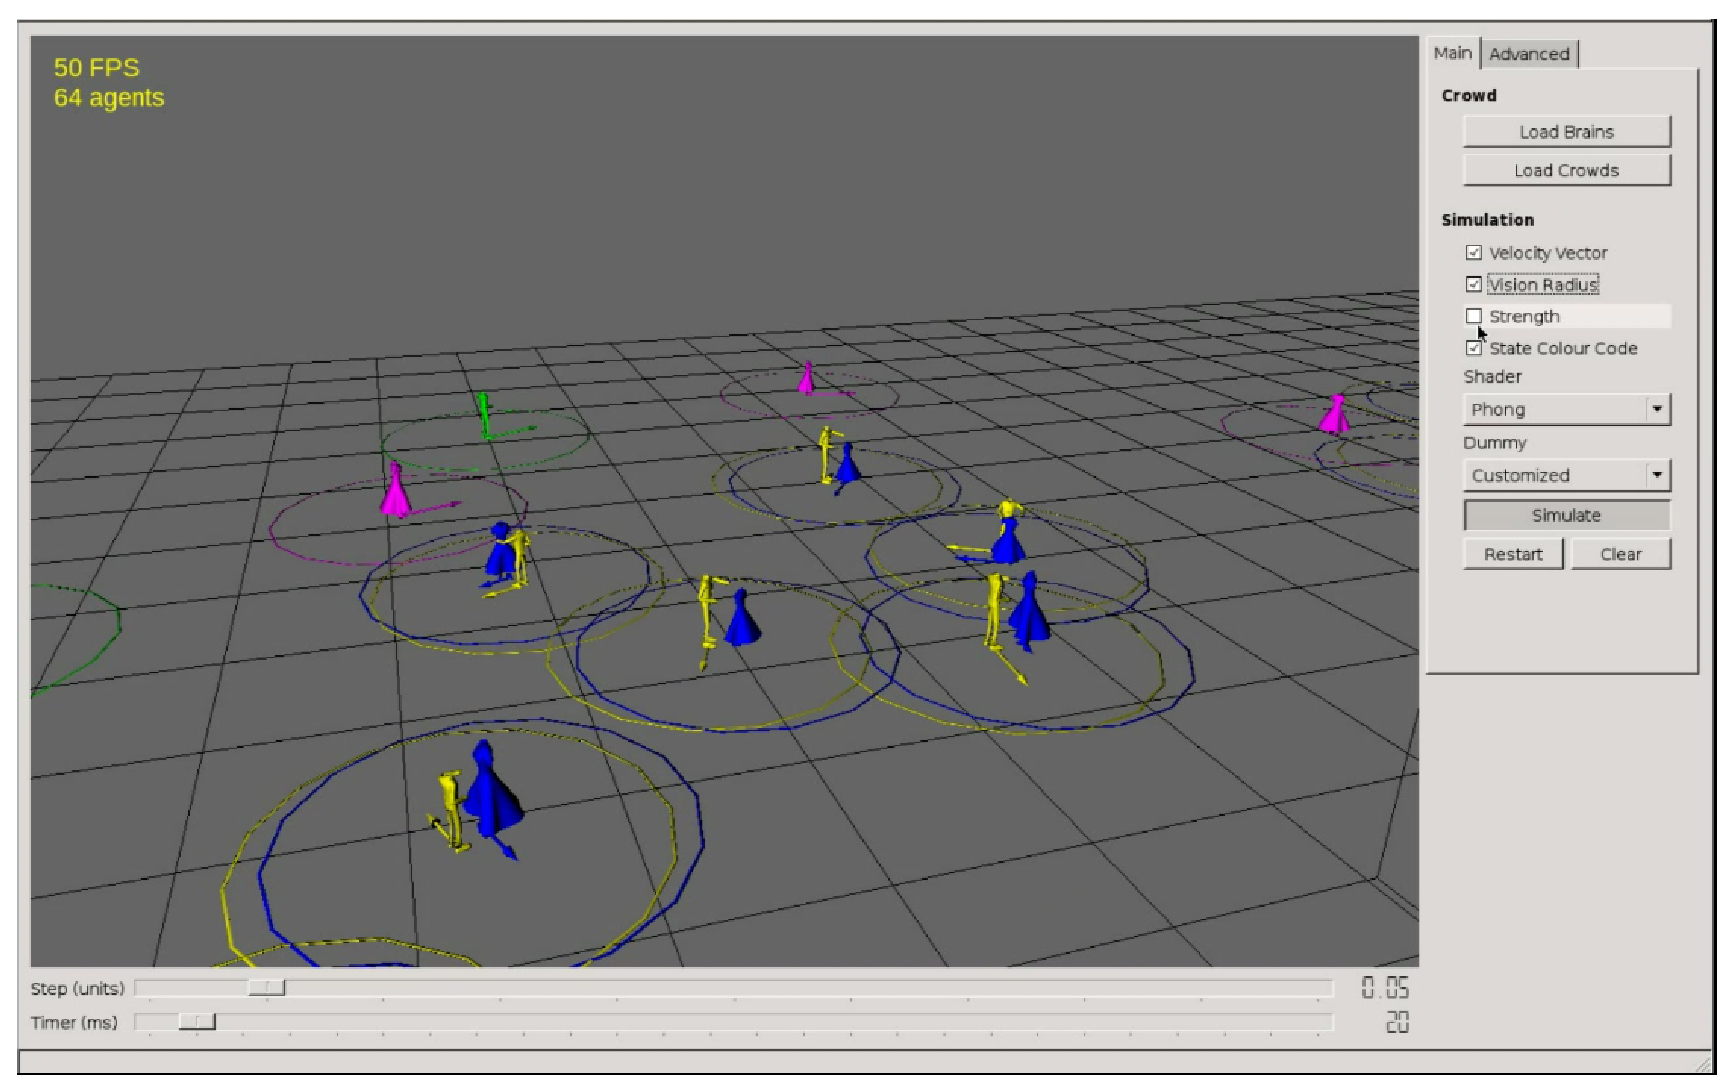
\includegraphics[scale=0.25]{ballroom_02.eps}} \\
 \end{tabular}
  \caption{A Ballroom Simulation}
  \label{fig:ballroomCaptures}
\end{figure}

\newpage
\subsection{One vs Many}

In this scenario, there is one agent who has to avoid many other agents that try to reach him. Combining forces which keep him anchored to the centre and which attacks to the incoming enemies this brain was written. If this agent, feels surrounded, he uses a super-attack to get rid of many enemies at the same time.

The brain of the enemies uses a simple state machine which distinguishes among the states of goingToTheMiddle, attacking and onAir. This last state allows to the enemies to know if they are in the air falling after a super attack.

\begin{figure}[!h]
  \centering
  \begin{tabular}{c c}
  	\subfloat[Blocking attacks of multiple enemies]{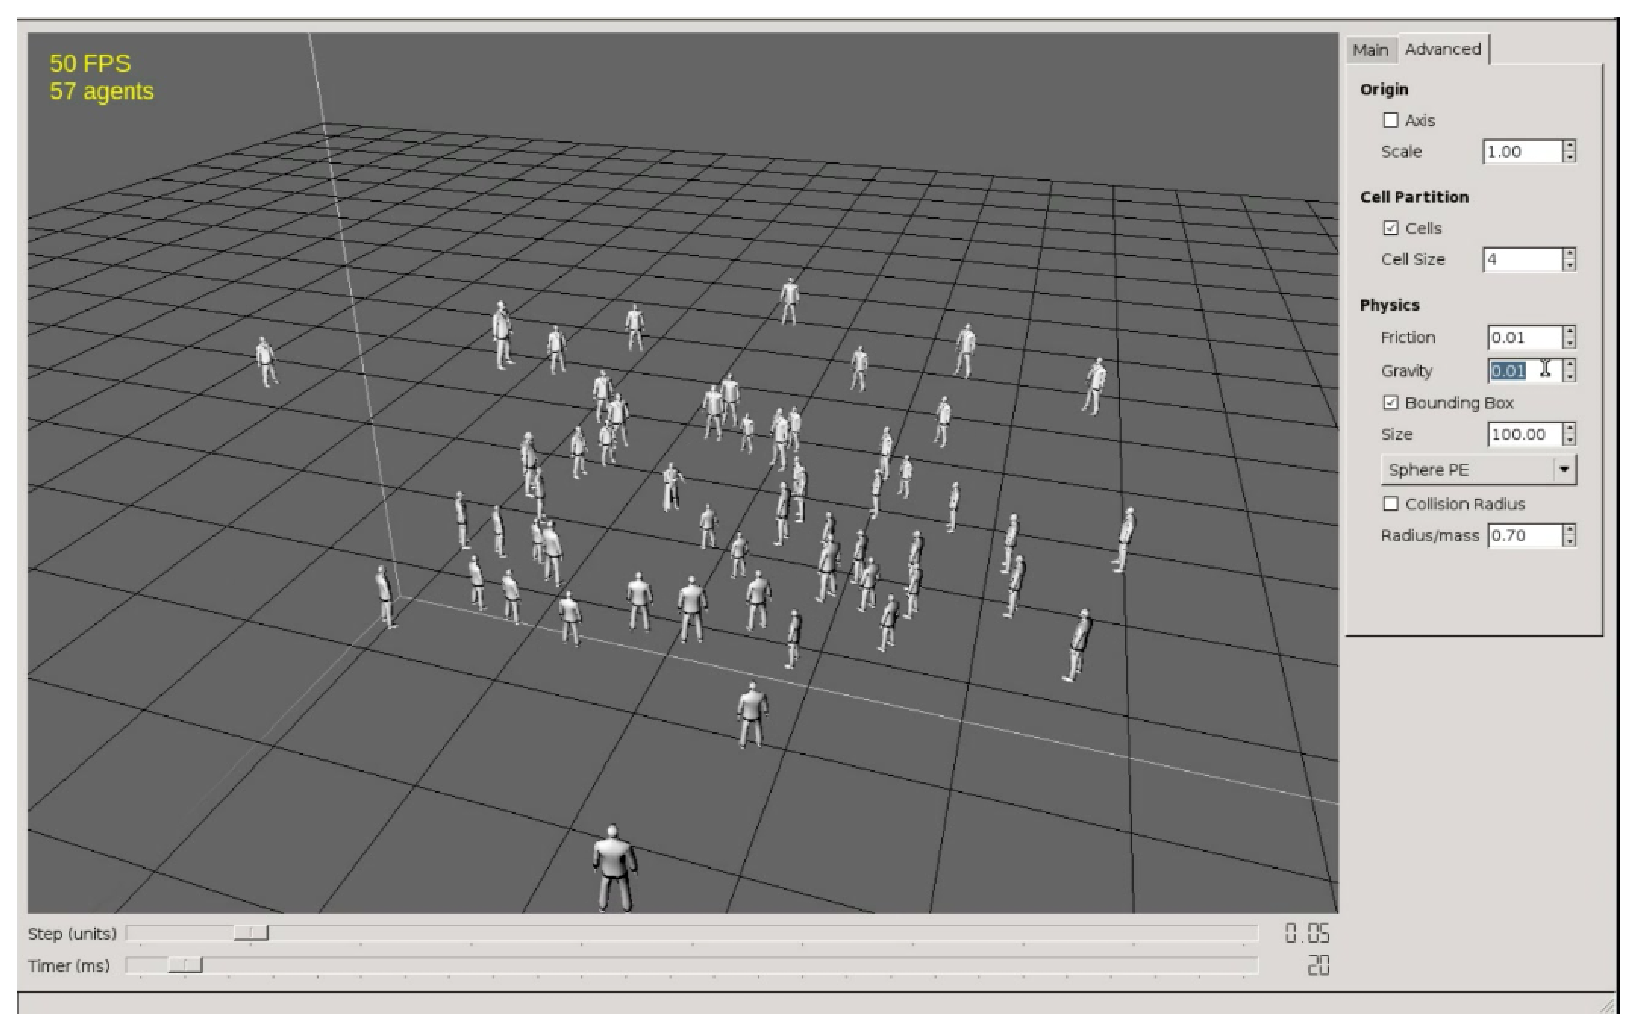
\includegraphics[scale=0.275]{matrix_01.eps}} &
 	\subfloat[Super attack to get rid of many enemies]{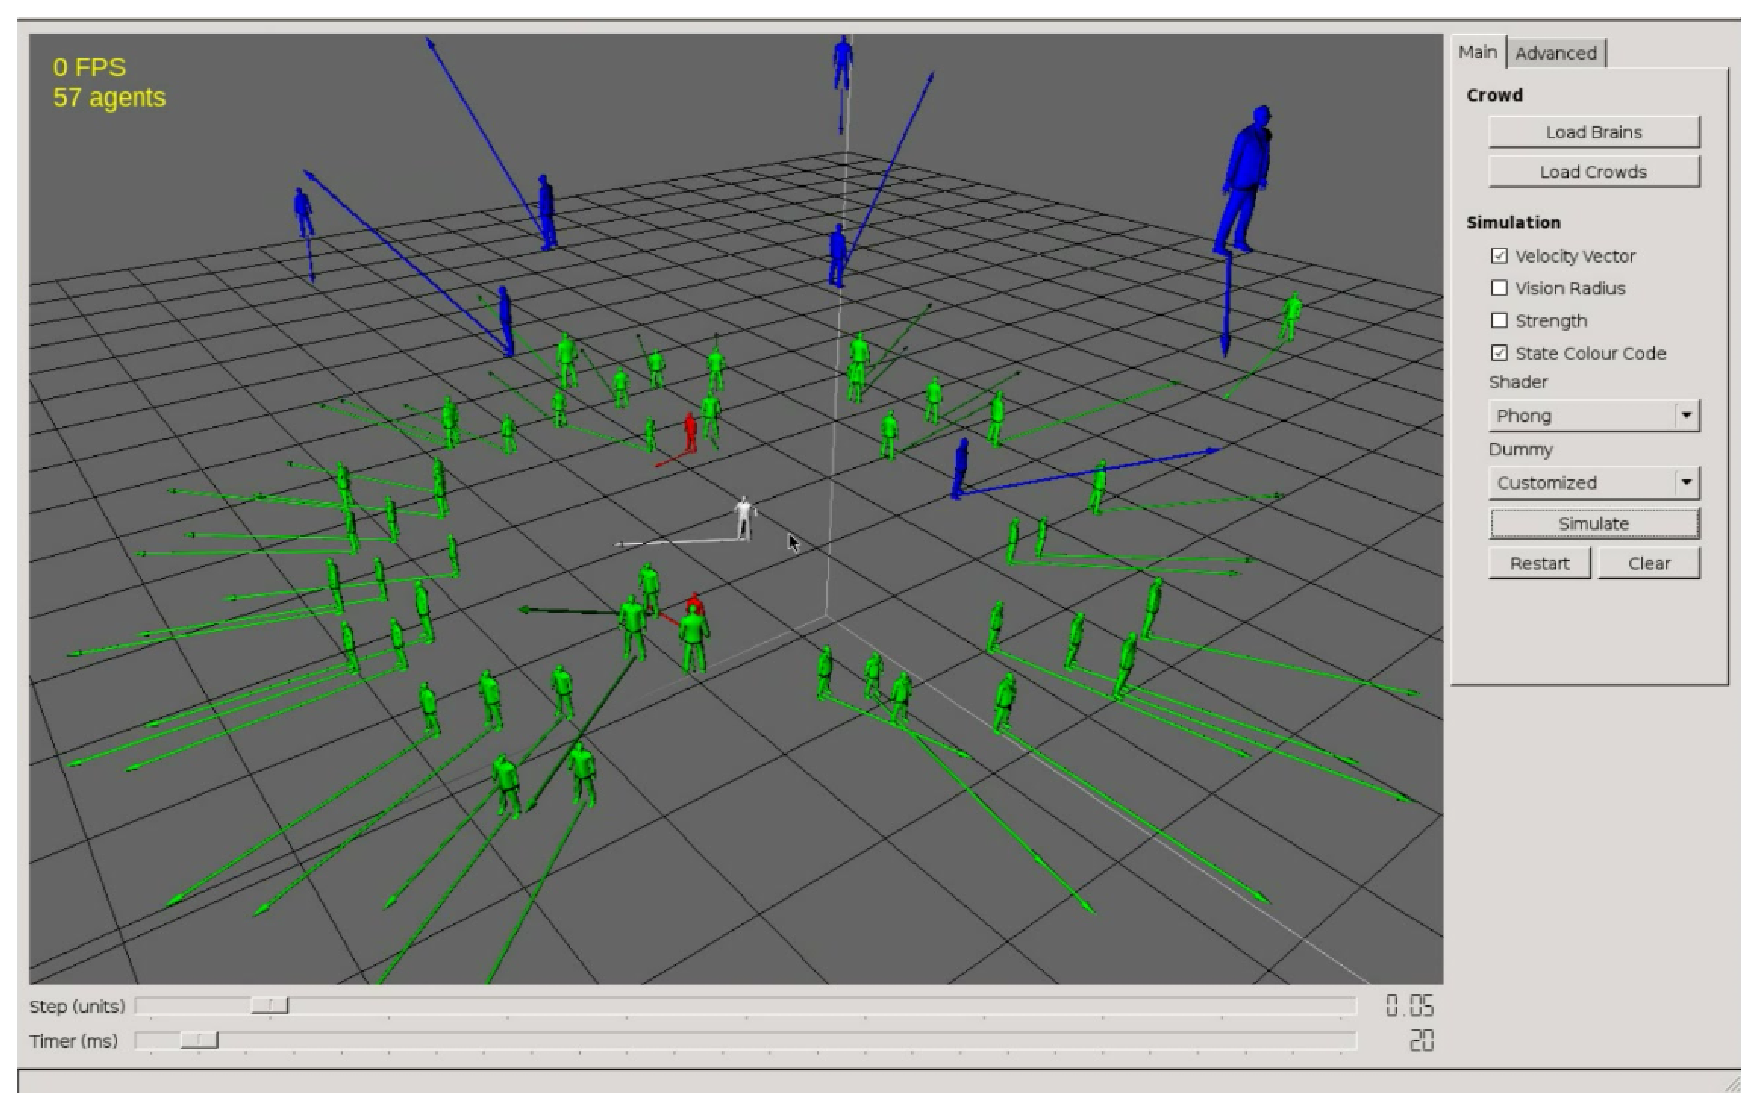
\includegraphics[scale=0.25]{matrix_02.eps}} \\
 \end{tabular}
  \caption{One vs Many Simulation}
  \label{fig:matrixCaptures}
\end{figure}

\subsection{Jumping Party}

This is another simple behaviour which includes 2 state FSM. One of the states is onFloor, which will produce an impulse to generate a jump, and the other is onAir, which works as in the last example.

\begin{figure}[!h]
  \centering
  \begin{tabular}{c c}
  	\subfloat[Jumpers' states]{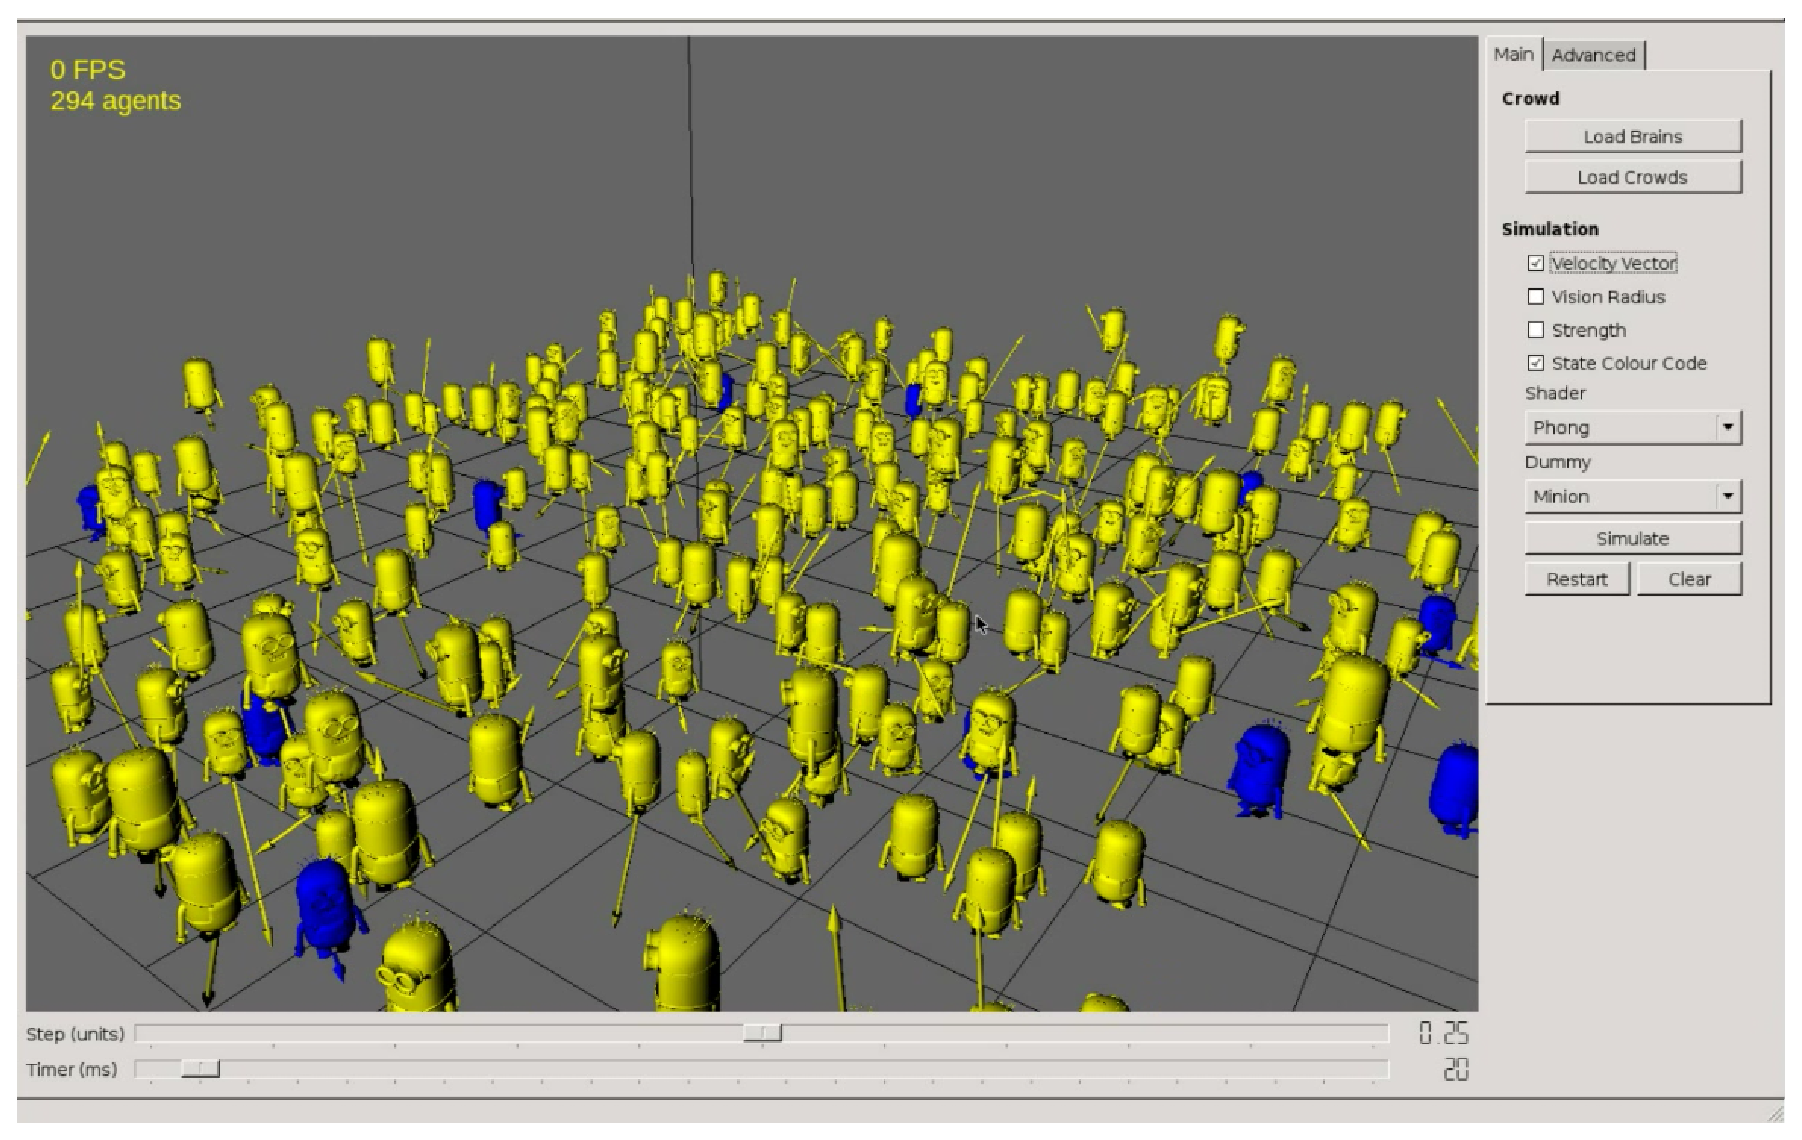
\includegraphics[scale=0.25]{minions_01.eps}} &
 	\subfloat[Jumping dummies]{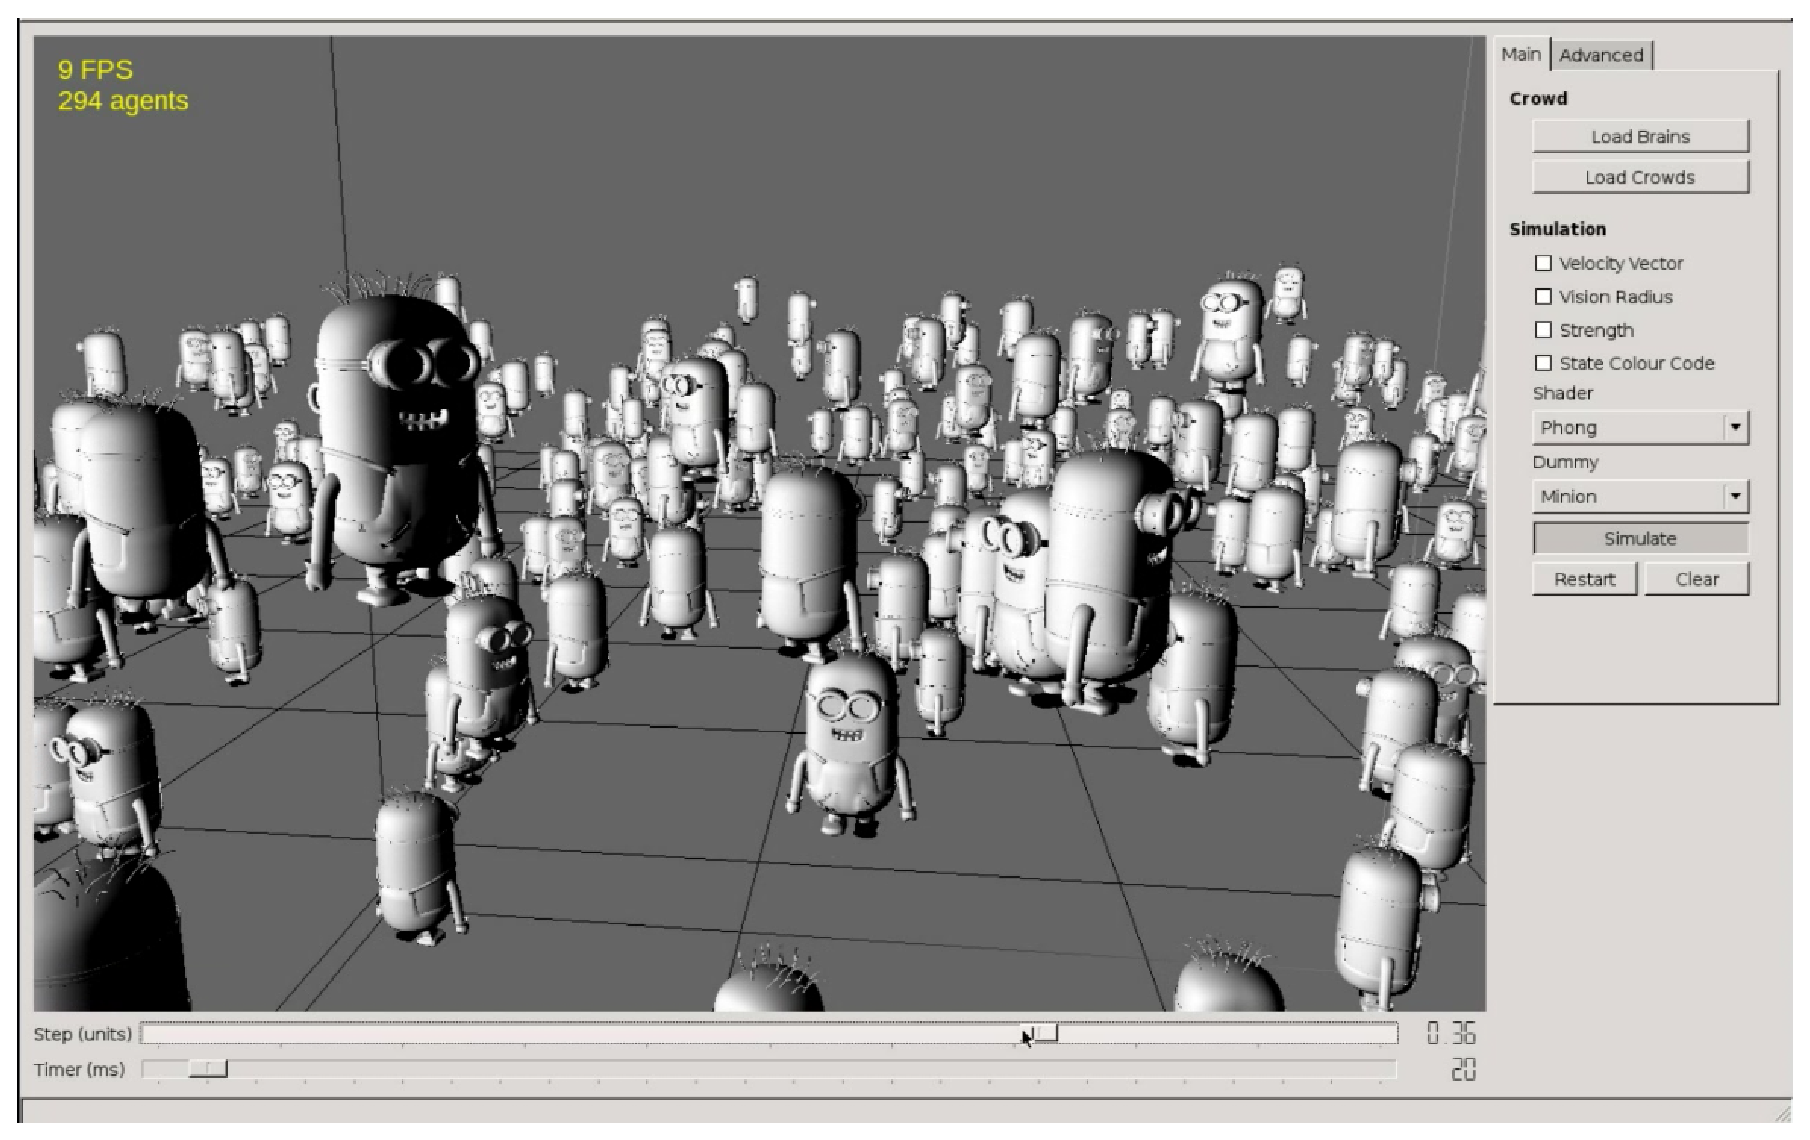
\includegraphics[scale=0.25]{minions_02.eps}} \\
 \end{tabular}
  \caption{Jumping Party Simulation}
  \label{fig:droidsCaptures}
\end{figure}


\ifx\isEmbedded\undefined
% References
\addcontentsline{toc}{chapter}{References}
\bibliographystyle{../ref/harvard}
\bibliography{../ref/master}
\pagebreak
\end{document}
\fi
\ifx\isEmbedded\undefined

\documentclass[12pt]{report}
	
% FONT RELATED
%\usepackage{times} %Move to times font
\usepackage[labelfont=bf,textfont=it]{caption}
\usepackage[utf8]{inputenc}

% LINKS, PAGE OF CONTENT, REF AND CROSS-REF, HEADERS/FOOTERS
\usepackage[hidelinks]{hyperref}
\usepackage{fancyhdr}
\usepackage{acronym}

% FIGURES, GRAPHICS, TABLES
\usepackage{graphicx}
\usepackage{parskip}
%\usepackage{subfigure}
\usepackage{subfig}
\usepackage{wrapfig}
\usepackage{subfloat}

% COLOURS, TEXT AND FORMATTING
\usepackage{array}
\usepackage{color}
\usepackage{setspace}
\usepackage{longtable}
\usepackage{multirow}

% ADVANCED MATHS, PSEUDO-CODE
\usepackage{amsmath}
\usepackage{alltt}
\usepackage{amsfonts}

% ALGORITHMS
\usepackage{algorithm}
\usepackage{algorithmic}

% LANDSCAPE FOR CLASS DIAGRAM
\usepackage{pdflscape}

% BIBLIOGRAPHY
\usepackage[authoryear]{natbib}
\bibpunct{(}{)}{;}{a}{,}{,}

% USE IN DISSER:

\setlength\oddsidemargin{0.85cm}
\setlength\evensidemargin{0.85cm}

\setlength\textheight{21.0cm}
\setlength\textwidth{15.0cm}

% indent at each new paragrapg
\setlength\parindent{0.5cm}

\setlength\topmargin{-0.2in}
\renewcommand{\baselinestretch}{1.3}

%REPORT

%\setlength\oddsidemargin{1cm}
%\setlength\evensidemargin{0.3in}
%%\setlength\headsep{2.5in}
%
%\setlength\textheight{9.0in}
%\setlength\textwidth{5.5in}
%
%% indent at each new paragrapg
%\setlength\parindent{0.5cm}
%
%%\setlength{\parskip}{10.5ex}
%
%\setlength\topmargin{-0.2in}

%\newcommand{\HRule}{\rule{\linewidth}{0.5mm}}
\newcommand{\HRule}{\rule{\linewidth}{0.0mm}}

% Color definitions (RGB model)
\definecolor{ms-comment}{rgb}{0.1, 0.4, 0.1}
\definecolor{ms-question}{rgb}{0.4, 0.0, 0.0}
\definecolor{ms-new}{rgb}{0.2, 0.4, 0.8}


\graphicspath{{../img/}}
\begin{document}
\fi

\chapter{Application Design and Implementation}
\label{chap:application_design_implementation}

\section{Design}

\begin{landscape}

\begin{figure}[!htb]
  \centering
  \includegraphics[scale=0.18]{classDiagram.eps}
  \caption{Class Diagram of the Application}
  \label{fig:classDiag}
\end{figure}

\end{landscape}

\section{Implementation}


\ifx\isEmbedded\undefined
% References
\addcontentsline{toc}{chapter}{References}
\bibliographystyle{../ref/harvard}
\bibliography{../ref/master}
\pagebreak
\end{document}
\fi

\ifx\isEmbedded\undefined

\documentclass[12pt]{report}
	
% FONT RELATED
%\usepackage{times} %Move to times font
\usepackage[labelfont=bf,textfont=it]{caption}
\usepackage[utf8]{inputenc}

% LINKS, PAGE OF CONTENT, REF AND CROSS-REF, HEADERS/FOOTERS
\usepackage[hidelinks]{hyperref}
\usepackage{fancyhdr}
\usepackage{acronym}

% FIGURES, GRAPHICS, TABLES
\usepackage{graphicx}
\usepackage{parskip}
%\usepackage{subfigure}
\usepackage{subfig}
\usepackage{wrapfig}
\usepackage{subfloat}

% COLOURS, TEXT AND FORMATTING
\usepackage{array}
\usepackage{color}
\usepackage{setspace}
\usepackage{longtable}
\usepackage{multirow}

% ADVANCED MATHS, PSEUDO-CODE
\usepackage{amsmath}
\usepackage{alltt}
\usepackage{amsfonts}

% ALGORITHMS
\usepackage{algorithm}
\usepackage{algorithmic}

% LANDSCAPE FOR CLASS DIAGRAM
\usepackage{pdflscape}

% BIBLIOGRAPHY
\usepackage[authoryear]{natbib}
\bibpunct{(}{)}{;}{a}{,}{,}

% USE IN DISSER:

\setlength\oddsidemargin{0.85cm}
\setlength\evensidemargin{0.85cm}

\setlength\textheight{21.0cm}
\setlength\textwidth{15.0cm}

% indent at each new paragrapg
\setlength\parindent{0.5cm}

\setlength\topmargin{-0.2in}
\renewcommand{\baselinestretch}{1.3}

%REPORT

%\setlength\oddsidemargin{1cm}
%\setlength\evensidemargin{0.3in}
%%\setlength\headsep{2.5in}
%
%\setlength\textheight{9.0in}
%\setlength\textwidth{5.5in}
%
%% indent at each new paragrapg
%\setlength\parindent{0.5cm}
%
%%\setlength{\parskip}{10.5ex}
%
%\setlength\topmargin{-0.2in}

%\newcommand{\HRule}{\rule{\linewidth}{0.5mm}}
\newcommand{\HRule}{\rule{\linewidth}{0.0mm}}

% Color definitions (RGB model)
\definecolor{ms-comment}{rgb}{0.1, 0.4, 0.1}
\definecolor{ms-question}{rgb}{0.4, 0.0, 0.0}
\definecolor{ms-new}{rgb}{0.2, 0.4, 0.8}


\graphicspath{{../img/}}
\begin{document}
%\maketitle
\fi

\chapter{Conclusion}
\label{chap:conclusion}

Your conclusion should be structured like this. An introductory sentence then:

\section{Summary}

A summary of what has been achieved.

\begin{itemize}
\item Bullet points are good to clarify
\item Bullet points are fun
\item I ran out of ideas
\end{itemize}

\section{Known bugs and issues}

This is optional, some people put it in future work, I think it is better to have a separate section for it. Issues and bugs are different. Bugs are unexpected behaviour in the program, something not running as it should. Issues are more due to algorithm limitations. If the algorithm only works for meshes of less than 100k polygons, it is a limitation, not a bug. A program crashing if you move around in a particular order is a bug. A render becoming ugly just on that particular spot in space, is a bug too.

\section{Future work}

What should be done in the future, what you would like to do.

\begin{itemize}
\item Become an astronaut
\item Go out
\item Make it work for real
\end{itemize}


\ifx\isEmbedded\undefined
% References
\addcontentsline{toc}{chapter}{References}
\bibliographystyle{../ref/harvard}
\bibliography{../ref/master}
\pagebreak
\end{document}
\fi

% References
% For my references I use JabRef.
% You can also use a simple text editor.
% Empty my file and fill it with your references
% Most publications have a bibtex "entry" available. 
% ACM Portal has a little beige box on the right which contains a link "Bibtex". This is what you copy paste in your file.
% ALL journal websites have something like this.
% I have left my references in case you need to reference a website or something else.
\addcontentsline{toc}{chapter}{References}
\bibliographystyle{ref/harvard}
\bibliography{ref/master}
\pagebreak

% Appendices
% This is the boring and lengthy stuff.
%
\appendix

You can have different appendices (A. B. etc...) and sub sections too.


\end{document}
